\chapter{Πειραματικά αποτελέσματα}
\section{Περιγραφή πειραμάτων}
Στόχος της παρούσας ενότητας είναι ο έλεγχος του συστήματος Automated Data Scientist, καθώς και της συνεισφοράς των τεχνικών που εφαρμόσαμε και περιγράψαμε στην Ενότητα \ref{sec:techniques}. Προς αυτό το σκοπό σχεδιάσαμε τα ακόλουθα πειράματα, τα οποία θα αναλύσουμε στη συνέχεια:
\begin{itemize}
	\item \textbf{σχεδιασμός μετρικής για ανίχνευση εξωκείμενων σετ δεδομένων}
	\item \textbf{αξιολόγηση των HPP μοντέλων}
	\item \textbf{αξιολόγηση του ensemble με προς-τα-εμπρός επιλογή μοντέλων}
	\item \textbf{συνολική αξιολόγηση του συστήματος}
\end{itemize}

\paragraph{Περιγραφή σετ δεδομένων} Για τη διεξαγωγή των πειραμάτων συλλέξαμε ένα πλήθος 123 σετ δεδομένων από διάφορες πηγές. (Στο παράρτημα \ref{appendix:Datasets} βρίσκεται ένας λεπτομερής κατάλογος περιγραφής τους.) Άξονας αναζήτησης κατά τη συλλογή ήταν η εύρεση σετ δεδομένων δυαδικής ταξινόμησης με ετερογενή χαρακτηριστικά, ώστε ο έλεγχος του συστήματος να είναι αντιπροσωπευτικός για το πραγματικό πλήθος σετ δεδομένων. Προκειμένου να υπάρχει μία κοινή διεπαφή για τα πειράματα ήταν απαραίτητος ο "καθαρισμός" των σετ δεδομένων μέσω των ακόλουθων βημάτων:
\begin{itemize}
	\item \textbf{μετατροπή αρχείων σε comma-delimited .csv} Τα πηγαία αρχεία βρίσκονταν σε μορφές .csv, .txt, .xlsx, .arff και .mysql.
	\item \textbf{καθορισμός κλάσης} Στη πλειοψηφία των περιπτώσεων η κλάση αναγνωριζόταν χειροκίνητα από την περιγραφή του σετ δεδομένων. Συλλέχθηκαν και σετ δεδομένων που ήταν πολλαπλής ταξινόμησης και παλινδρόμησης. Στην πρώτη περίπτωση έγινε αντιστοίχηση σε δύο ουσιώδεις κλάσεις, ενώ στη δεύτερη βρέθηκε η μέση τιμή της μεταβλητής κλάσης και χρησιμοποιήθηκε ως κατώφλι για το διαχωρισμό των παραδειγμάτων σε δύο κλάσεις.
	\item \textbf{αναγνώριση άγνωστων τιμών} Στα αρχεία που περιείχαν άγνωστες τιμές χρησιμοποιούνταν διάφοροι συμβολισμοί ("?", "*", "") οι οποίοι αντικαταστάθηκαν από κενά, ώστε να αναγνωρίζονται από την R ως NAs (Not Available).  
\end{itemize}
\section{Σχεδιασμός μετρικής για ανίχνευση εξωκείμενων σετ δεδομένων}
Το σύστημα Automated Data Scientist απευθύνεται σε οποιοδήποτε σετ δεδομένων δυαδικής ταξινόμησης. ένα σύνολο πολύ ετερογενές ως προς πεδίο εφαρμογής, φύση χαρακτηριστικών, μέγεθος κλπ. Καθώς το σύστημά μας περιέχει μετα-μάθηση, έχουμε συλλέξει και εκπαιδευτεί σε μια αποθήκη σετ δεδομένων, η οποία αντιπροσωπεύει το κομμάτι του "κόσμου" για το οποίο έχουμε μετα-γνώση. Όταν ο χρήστης τροφοδοτεί το σύστημά μας με ένα νέο σετ δεδομένων υπάρχει το ενδεχόμενο αυτό να βρίσκεται σε ένα ανεξερεύνητο κομμάτι του "κόσμου" με αποτέλεσμα το πείραμα να είναι υποβέλτιστο. Αποτελεί λοιπόν λειτουργική απαίτηση του συστήματος ο υπολογισμός μίας μετρικής, η οποία θα εκφράζει την έλλειψη ετοιμότητας του συστήματός μας να βελτιστοποιήσει ένα άγνωστο σετ δεδομένων.


\section{Αξιολόγηση της τεχνικής βελτιστοποίησης υπερ-παραμέτρων με μετα-μάθηση και χρήση διαστημάτων πρόβλεψης}
Όπως είδαμε στην ενότητα \ref{sec:HPP} προϊόντα αυτής της τεχνικής είναι τα \gls{HPP} μοντέλα, καθένα εκ των οποίων έχει εκπαιδευτεί στη πρόβλεψη μίας υπερ-παραμέτρου ενός αλγορίθμου μηχανικής μάθησης. Σε αυτό το σημείο θα αξιολογήσουμε τα μοντέλα αυτά ως προς το σκοπό τους, δηλαδή πόσο καλά προβλέπουν τις βελτιστοποιημένες υπερ-παραμέτρους. Επίσης, θα σχολιάσουμε τη συνεισφορά της χρήσης διαστημάτων πρόβλεψης.

Για την παραγωγή των σετ μετα-δεδομένων, τα οποία χρησιμοποιούνται για την εκπαίδευση των HPP μοντέλων, είναι απαραίτητα δύο στάδια:
\begin{itemize}
	\item Εξαγωγή των μετα-χαρακτηριστικών κάθε σετ δεδομένων. Τα  81 μετα-χαρακτηριστικά που χρησιμοποιήσαμε περιγράφονται στον Πίνακα \ref{table:meta} και υπολογίστηκαν με χρήση του πακέτου mf\-Extractor του συστήματός μας. Βασίστηκαν σε εκτεταμένη βιβλιογραφική έρευνα και προσπαθούν να συμπεριλάβουν όλα τα είδη μετα-χαρακτηριστικών που εμφανίζονται σε παρόμοιες εργασίες (\citep{Brazdil2009,Reif_meta2-features:,Feurer:2014:UMI:3015544.3015549}).~\footnote{Πριν τον υπολογισμό τους έγινε μετατροπή των κατηγορικών χαρακτηριστικών σε μεταβλητές-δείκτες, ώστε να υπάρχει ομοιόμορφη αντιμετώπιση.}   
		\begin{table}[!htb]
			\begin{center}
				\caption{Λίστα μετα-χαρακτηριστικών, τα οποία χρησιμοποιήθηκαν για την εκπαίδευση των HPP μοντέλων}
				\label{table:meta}
				\scalebox{0.7}{
				\begin{tabular}{ |l|l| } 
					\hline
					\textbf{Απλά} & \textbf{Στατιστικά Aριθμητικά}  \\
					Πλήθος χαρακτηριστικών & Άθροισμα \\
					Λογάριθμος πλήθους χαρακτηριστικών & Μέση τιμή \\
					Πλήθος παραδειγμάτων & Τυπική απόκλιση \\
					Λογάριθμος πλήθους παραδειγμάτων &Ελάχιστη τιμή \\
					Πλήθος χαρακτηριστικών με άγνωστες τιμές &Μέγιστη τιμή \\
					Ποσοστό πλήθους χαρακτηριστικών με άγνωστες τιμές& Κυρτότητα\\
					Πλήθος παραδειγμάτων με άγνωστες τιμές & Λοξότητα\\
					Ποσοστό πλήθους παραδειγμάτων με άγνωστες τιμές &  Ποσοστό \gls{PC}s για $95\%$ διακύμανση\\
					Πλήθος άγνωστων τιμών &Κυρτότητα πρώτης \gls{PC} \\
					Λογάριθμος πλήθους άγνωστων τιμών&Λοξότητα πρώτης \gls{PC} \\
					Πλήθος αριθμητικών χαρακτηριστικών &  \\
					Πλήθος κατηγορικών χαρακτηριστικών & \textbf{Στατιστικά Kατηγορικά}\\
					Πιθανότητες κλάσης & Πλήθος επιπέδων \\
					Ελάχιστη πιθανότητα κλάσης & \\
					Μέγιστη πιθανότητα κλάσης & \textbf{Μετα2-}\\
					Μέση τιμή πιθανοτήτων κλάσης& Άθροισμα\\
					Τυπική απόκλιση πιθανοτήτων κλάσης & Μέση τιμή\\
					& Τυπική απόκλιση\\
					\textbf{Θεωρίας Πληροφορίας}  & Ελάχιστη τιμή\\
					Εντροπία Κλάσης & Μέγιστη τιμή\\
				    &	 Κυρτότητα\\
				    & Λοξότητα\\				
					\hline
				\end{tabular}}   
			\end{center}
				\end{table}
				
Καθώς το πλήθος των μετα-χαρακτηριστικών είναι δυσανάλογο των διαθέσιμων σετ δεδομένων για εκπαίδευση των \gls{HPP} μοντέλων, θα επιστρατευθούν τεχνικές επιλογής των βέλτιστων. Σε πρώτη φάση αφαιρέσαμε τα γραμμικά συσχετισμένα χαρακτηριστικά, όπως αυτά υπολογίστηκαν στο σετ δεδομένων εκπαίδευσης. H τελική λίστα παρουσιάζεται στον Πίνακα \ref{table:meta2}:	

	 \begin{table}[!htb]
	 	\footnotesize
	 	\begin{center}
	 		\caption{Λίστα μετα-χαρακτηριστικών μετά από εφαρμογή φιλτραρίσματος}
	 		\label{table:meta2}
	 		\begin{tabular}{ |l|l| } 
	 			\hline
	 		     Άθροισμα αθροισμάτων & Τυπική απόκλιση επιπέδων    \\
	 			Άθροισμα μέγιστων τιμών &  Κυρτότητα επιπέδων  \\
	 			Μέση τιμή τυπικών αποκλίσεων  & Λοξότητα επιπέδων    \\
	 		    Μέση τιμή ελαχίστων τιμών &  Πλήθος χαρακτηριστικών  \\
	 			Μέση τιμή κυρτοτήτων &   Λογάριθμος πλήθους χαρακτηριστικών \\
	 			Μέση τιμή λοξοτήτων &    Πλήθος παραδειγμάτων\\
	 			Τυπική απόκλιση ελαχίστων τιμών & Λογάριθμος πλήθους παραδειγμάτων   \\
	 			Ελάχιστη τιμή μέσων τιμών &  Ποσοστό αγνώστων τιμών  \\
	 			Ελάχιστη τιμή τυπικών αποκλίσεων &  Πλήθος αριθμητικών χαρακτηριστικών  \\
	 			Ελάχιστη τιμή ελαχίστων τιμών &  Πλήθος κατηγορικών χαρακτηριστικών  \\
	 			Ελάχιστη τιμή μεγίστων τιμών &  Μέγιστη πιθανότητα κλάσης    \\
	 			Ελάχιστη τιμή λοξοτήτων & Μέση τιμή πιθανοτήτων κλάσης   \\
	 			Κυρτότητα ελαχίστων τιμών & Ποσοστό \gls{PC} για $95\%$ διακύμανση  \\
	 			Κυρτότητα μεγίστων τιμών & Κυρτότητα πρώτης \gls{PC}   \\
	 			Λοξότητα λοξοτήτων & Λοξότητα \gls{PC}   \\
	 		    Άθροισμα επιπέδων &    \\
	 			\hline
	 		\end{tabular}    
	 	\end{center}
	 \end{table}
	\FloatBarrier
	\item Εύρεση των βέλτιστων υπερ-παραμέτρων για κάθε αλγόριθμο. Προς αυτό το σκοπό χρησιμοποιήθηκε η βιβλιοθήκη HPOlib, την οποία έχουμε περιγράψει στην Eνότητα \ref{section:tools}. Ο αλγόριθμος που επιλέχθηκε ήταν ο Tree Parzen Estimator, καθώς είναι σημαντικά ταχύτερος από τους υπόλοιπους. Από τη πλευρά μας ήταν απαραίτητος ο ορισμός του χώρου αναζήτησης υπερ-παραμέτρων και της συνάρτησης κόστους για κάθε αλγόριθμο, η οποία ορίστηκε ως $ Cost = 1- Accuracy$. Στον Πίνακα \ref{table:algorithms} μπορούμε να δούμε τους αλγορίθμους μάθησης με τους οποίους ασχοληθήκαμε, καθώς και τις υπερ-παραμέτρους τους.

\end{itemize}
	\begin{table}[!htb]
		\begin{center}
				\caption[Οι αλγόριθμοι που χρησιμοποιεί το σύστημα Automated Data Scientist και οι υπερ-παράμετροί του]{Οι αλγόριθμοι που χρησιμοποιεί το σύστημα Automated Data Scientist και οι υπερ-παράμετροί τους, όπως τις ορίζει το πακέτο caret. knn: κ-κοντινότερος γείτονας, rpart: δέντρο ταξινόμησης και παλινδρόμησης (CART), nnet: \gls{ΤΝΔ}, svmRadial: \gls{SVM} με χρήση γκαουσιανού πυρήνα.}
				\label{table:algorithms}
			\begin{tabular}{ |c|c|c|c| } 
				\hline
				knn & rpart & nnet & svmRadial \\
				\hline
			    k & cp & size& C \\
			     &  & decay& sigma  \\
				\hline
			\end{tabular}    
		\end{center}
	\end{table} 
	
Στα πειράματα που ακολουθούν έχουμε χρησιμοποιήσει τη τεχνική leave one out για την αξιολόγηση των μοντέλων, 10-fold cross-validation για τη ρύθμιση και ως κριτήριο της απόδοσης των μοντέλων παλινδρόμησης τη ρίζα του μέσου τετραγωνικού σφάλματος (root mean squared error).

Όσο αφορά τις τεχνικές προ-επεξεργασίας που χρησιμοποιήθηκαν: ως μέθοδο φιλτραρίσματος για επιλογή χαρακτηριστικών ορίζουμε την επιλογή των λιγότερο συσχετισμένων χαρακτηριστικών με βάση τη γραμμική συσχέτιση. Η προς-τα-εμπρός επιλογή χαρακτηριστικών γίνεται με χρήση του πακέτου Boruta~\footnote{https://cran.r-project.org/web/packages/Boruta/Boruta.pdf} και της συνάρτησης rfe του πακέτου caret. Τέλος, ο υπολογισμός των διαστημάτων πρόβλεψης γίνεται με τη τεχνική του bootstrapping, η οποία περιγράφεται στο Παράρτημα \ref{appendix:Intervals}.
 
\subsection{Πρόβλεψη υπερ-παραμέτρου πλήθους γειτόνων για αλγόριθμο k-κοντι\-νότερου γείτονα}

\paragraph{Περιγραφή προβλήματος} Η υπερ-παράμετρος κ στον αλγόριθμο κ-κοντινότερου γείτονα ορίζει πόσα από τα κοντινότερα παραδείγματα θα ληφθούν υπόψιν κατά την πρόβλεψη. Πρόκειται για μία ακέραια και θετική τιμή, το ιστόγραμμα της οποίας, μετά από τη βελτιστοποίησή της στο σετ δεδομένων εκπαίδευσης φαίνεται στο σχήμα  \ref{fig:ktpehist} για βελτιστοποίηση με χρήση του αλγορίθμου \gls{TPE} και στο \ref{fig:kgridhist} για βελτιστοποίηση με πλεγματική αναζήτηση.

\begin{figure}[!htb]
	\begin{minipage}{0.48\textwidth}
						\scalebox{0.4}{
							
\begin{tikzpicture}[x=1pt,y=1pt]
\definecolor{fillColor}{RGB}{255,255,255}
\path[use as bounding box,fill=fillColor,fill opacity=0.00] (0,0) rectangle (505.89,361.35);
\begin{scope}
\path[clip] (  0.00,  0.00) rectangle (505.89,361.35);
\definecolor{drawColor}{RGB}{0,0,0}

\node[text=drawColor,anchor=base,inner sep=0pt, outer sep=0pt, scale=  1.20] at (264.94,332.61) {\bfseries Histogram of k};

\node[text=drawColor,anchor=base,inner sep=0pt, outer sep=0pt, scale=  1.00] at (264.94, 15.60) {k};

\node[text=drawColor,rotate= 90.00,anchor=base,inner sep=0pt, outer sep=0pt, scale=  1.00] at ( 10.80,186.67) {Frequency};
\end{scope}
\begin{scope}
\path[clip] (  0.00,  0.00) rectangle (505.89,361.35);
\definecolor{drawColor}{RGB}{0,0,0}

\path[draw=drawColor,line width= 0.4pt,line join=round,line cap=round] (109.57, 61.20) -- (464.71, 61.20);

\path[draw=drawColor,line width= 0.4pt,line join=round,line cap=round] (109.57, 61.20) -- (109.57, 55.20);

\path[draw=drawColor,line width= 0.4pt,line join=round,line cap=round] (198.36, 61.20) -- (198.36, 55.20);

\path[draw=drawColor,line width= 0.4pt,line join=round,line cap=round] (287.14, 61.20) -- (287.14, 55.20);

\path[draw=drawColor,line width= 0.4pt,line join=round,line cap=round] (375.92, 61.20) -- (375.92, 55.20);

\path[draw=drawColor,line width= 0.4pt,line join=round,line cap=round] (464.71, 61.20) -- (464.71, 55.20);

\node[text=drawColor,anchor=base,inner sep=0pt, outer sep=0pt, scale=  1.00] at (109.57, 39.60) {2};

\node[text=drawColor,anchor=base,inner sep=0pt, outer sep=0pt, scale=  1.00] at (198.36, 39.60) {4};

\node[text=drawColor,anchor=base,inner sep=0pt, outer sep=0pt, scale=  1.00] at (287.14, 39.60) {6};

\node[text=drawColor,anchor=base,inner sep=0pt, outer sep=0pt, scale=  1.00] at (375.92, 39.60) {8};

\node[text=drawColor,anchor=base,inner sep=0pt, outer sep=0pt, scale=  1.00] at (464.71, 39.60) {10};

\path[draw=drawColor,line width= 0.4pt,line join=round,line cap=round] ( 49.20, 70.49) -- ( 49.20,302.86);

\path[draw=drawColor,line width= 0.4pt,line join=round,line cap=round] ( 49.20, 70.49) -- ( 43.20, 70.49);

\path[draw=drawColor,line width= 0.4pt,line join=round,line cap=round] ( 49.20,109.22) -- ( 43.20,109.22);

\path[draw=drawColor,line width= 0.4pt,line join=round,line cap=round] ( 49.20,147.95) -- ( 43.20,147.95);

\path[draw=drawColor,line width= 0.4pt,line join=round,line cap=round] ( 49.20,186.68) -- ( 43.20,186.68);

\path[draw=drawColor,line width= 0.4pt,line join=round,line cap=round] ( 49.20,225.40) -- ( 43.20,225.40);

\path[draw=drawColor,line width= 0.4pt,line join=round,line cap=round] ( 49.20,264.13) -- ( 43.20,264.13);

\path[draw=drawColor,line width= 0.4pt,line join=round,line cap=round] ( 49.20,302.86) -- ( 43.20,302.86);

\node[text=drawColor,rotate= 90.00,anchor=base,inner sep=0pt, outer sep=0pt, scale=  1.00] at ( 34.80, 70.49) {0};

\node[text=drawColor,rotate= 90.00,anchor=base,inner sep=0pt, outer sep=0pt, scale=  1.00] at ( 34.80,109.22) {10};

\node[text=drawColor,rotate= 90.00,anchor=base,inner sep=0pt, outer sep=0pt, scale=  1.00] at ( 34.80,147.95) {20};

\node[text=drawColor,rotate= 90.00,anchor=base,inner sep=0pt, outer sep=0pt, scale=  1.00] at ( 34.80,186.68) {30};

\node[text=drawColor,rotate= 90.00,anchor=base,inner sep=0pt, outer sep=0pt, scale=  1.00] at ( 34.80,225.40) {40};

\node[text=drawColor,rotate= 90.00,anchor=base,inner sep=0pt, outer sep=0pt, scale=  1.00] at ( 34.80,264.13) {50};

\node[text=drawColor,rotate= 90.00,anchor=base,inner sep=0pt, outer sep=0pt, scale=  1.00] at ( 34.80,302.86) {60};
\end{scope}
\begin{scope}
\path[clip] ( 49.20, 61.20) rectangle (480.69,312.15);
\definecolor{drawColor}{RGB}{0,0,0}

\path[draw=drawColor,line width= 0.4pt,line join=round,line cap=round] ( 65.18, 70.49) rectangle (109.57,120.84);

\path[draw=drawColor,line width= 0.4pt,line join=round,line cap=round] (109.57, 70.49) rectangle (153.97, 74.37);

\path[draw=drawColor,line width= 0.4pt,line join=round,line cap=round] (153.97, 70.49) rectangle (198.36,302.86);

\path[draw=drawColor,line width= 0.4pt,line join=round,line cap=round] (198.36, 70.49) rectangle (242.75, 70.49);

\path[draw=drawColor,line width= 0.4pt,line join=round,line cap=round] (242.75, 70.49) rectangle (287.14, 70.49);

\path[draw=drawColor,line width= 0.4pt,line join=round,line cap=round] (287.14, 70.49) rectangle (331.53, 93.73);

\path[draw=drawColor,line width= 0.4pt,line join=round,line cap=round] (331.53, 70.49) rectangle (375.92, 74.37);

\path[draw=drawColor,line width= 0.4pt,line join=round,line cap=round] (375.92, 70.49) rectangle (420.32, 82.11);

\path[draw=drawColor,line width= 0.4pt,line join=round,line cap=round] (420.32, 70.49) rectangle (464.71,113.09);
\end{scope}
\end{tikzpicture}


}
							\captionsetup[subfigure]{width=0.8\textwidth}
							\caption{Ιστόγραμμα υπερ-παραμέτρου k για βελτιστοποίηση με \gls{TPE}.}
						\label{fig:ktpehist}
	\end{minipage}
	\begin{minipage}{0.48\textwidth}
						\scalebox{0.4}{
			
\begin{tikzpicture}[x=1pt,y=1pt]
\definecolor{fillColor}{RGB}{255,255,255}
\path[use as bounding box,fill=fillColor,fill opacity=0.00] (0,0) rectangle (505.89,361.35);
\begin{scope}
\path[clip] (  0.00,  0.00) rectangle (505.89,361.35);
\definecolor{drawColor}{RGB}{0,0,0}

\node[text=drawColor,anchor=base,inner sep=0pt, outer sep=0pt, scale=  1.20] at (264.94,332.61) {\bfseries Histogram of k};

\node[text=drawColor,anchor=base,inner sep=0pt, outer sep=0pt, scale=  1.00] at (264.94, 15.60) {k};

\node[text=drawColor,rotate= 90.00,anchor=base,inner sep=0pt, outer sep=0pt, scale=  1.00] at ( 10.80,186.67) {Frequency};
\end{scope}
\begin{scope}
\path[clip] (  0.00,  0.00) rectangle (505.89,361.35);
\definecolor{drawColor}{RGB}{0,0,0}

\path[draw=drawColor,line width= 0.4pt,line join=round,line cap=round] ( 65.18, 61.20) -- (464.71, 61.20);

\path[draw=drawColor,line width= 0.4pt,line join=round,line cap=round] ( 65.18, 61.20) -- ( 65.18, 55.20);

\path[draw=drawColor,line width= 0.4pt,line join=round,line cap=round] (165.06, 61.20) -- (165.06, 55.20);

\path[draw=drawColor,line width= 0.4pt,line join=round,line cap=round] (264.94, 61.20) -- (264.94, 55.20);

\path[draw=drawColor,line width= 0.4pt,line join=round,line cap=round] (364.83, 61.20) -- (364.83, 55.20);

\path[draw=drawColor,line width= 0.4pt,line join=round,line cap=round] (464.71, 61.20) -- (464.71, 55.20);

\node[text=drawColor,anchor=base,inner sep=0pt, outer sep=0pt, scale=  1.00] at ( 65.18, 39.60) {0};

\node[text=drawColor,anchor=base,inner sep=0pt, outer sep=0pt, scale=  1.00] at (165.06, 39.60) {5};

\node[text=drawColor,anchor=base,inner sep=0pt, outer sep=0pt, scale=  1.00] at (264.94, 39.60) {10};

\node[text=drawColor,anchor=base,inner sep=0pt, outer sep=0pt, scale=  1.00] at (364.83, 39.60) {15};

\node[text=drawColor,anchor=base,inner sep=0pt, outer sep=0pt, scale=  1.00] at (464.71, 39.60) {20};

\path[draw=drawColor,line width= 0.4pt,line join=round,line cap=round] ( 49.20, 70.49) -- ( 49.20,302.86);

\path[draw=drawColor,line width= 0.4pt,line join=round,line cap=round] ( 49.20, 70.49) -- ( 43.20, 70.49);

\path[draw=drawColor,line width= 0.4pt,line join=round,line cap=round] ( 49.20,116.97) -- ( 43.20,116.97);

\path[draw=drawColor,line width= 0.4pt,line join=round,line cap=round] ( 49.20,163.44) -- ( 43.20,163.44);

\path[draw=drawColor,line width= 0.4pt,line join=round,line cap=round] ( 49.20,209.91) -- ( 43.20,209.91);

\path[draw=drawColor,line width= 0.4pt,line join=round,line cap=round] ( 49.20,256.38) -- ( 43.20,256.38);

\path[draw=drawColor,line width= 0.4pt,line join=round,line cap=round] ( 49.20,302.86) -- ( 43.20,302.86);

\node[text=drawColor,rotate= 90.00,anchor=base,inner sep=0pt, outer sep=0pt, scale=  1.00] at ( 34.80, 70.49) {0};

\node[text=drawColor,rotate= 90.00,anchor=base,inner sep=0pt, outer sep=0pt, scale=  1.00] at ( 34.80,116.97) {5};

\node[text=drawColor,rotate= 90.00,anchor=base,inner sep=0pt, outer sep=0pt, scale=  1.00] at ( 34.80,163.44) {10};

\node[text=drawColor,rotate= 90.00,anchor=base,inner sep=0pt, outer sep=0pt, scale=  1.00] at ( 34.80,209.91) {15};

\node[text=drawColor,rotate= 90.00,anchor=base,inner sep=0pt, outer sep=0pt, scale=  1.00] at ( 34.80,256.38) {20};

\node[text=drawColor,rotate= 90.00,anchor=base,inner sep=0pt, outer sep=0pt, scale=  1.00] at ( 34.80,302.86) {25};
\end{scope}
\begin{scope}
\path[clip] ( 49.20, 61.20) rectangle (480.69,312.15);
\definecolor{drawColor}{RGB}{0,0,0}

\path[draw=drawColor,line width= 0.4pt,line join=round,line cap=round] ( 65.18, 70.49) rectangle (105.13,302.86);

\path[draw=drawColor,line width= 0.4pt,line join=round,line cap=round] (105.13, 70.49) rectangle (145.09,209.91);

\path[draw=drawColor,line width= 0.4pt,line join=round,line cap=round] (145.09, 70.49) rectangle (185.04,172.73);

\path[draw=drawColor,line width= 0.4pt,line join=round,line cap=round] (185.04, 70.49) rectangle (224.99,126.26);

\path[draw=drawColor,line width= 0.4pt,line join=round,line cap=round] (224.99, 70.49) rectangle (264.94, 79.79);

\path[draw=drawColor,line width= 0.4pt,line join=round,line cap=round] (264.94, 70.49) rectangle (304.90,135.56);

\path[draw=drawColor,line width= 0.4pt,line join=round,line cap=round] (304.90, 70.49) rectangle (344.85, 89.08);

\path[draw=drawColor,line width= 0.4pt,line join=round,line cap=round] (344.85, 70.49) rectangle (384.80,135.56);

\path[draw=drawColor,line width= 0.4pt,line join=round,line cap=round] (384.80, 70.49) rectangle (424.76,126.26);

\path[draw=drawColor,line width= 0.4pt,line join=round,line cap=round] (424.76, 70.49) rectangle (464.71,219.21);
\end{scope}
\end{tikzpicture}

}
			\captionsetup[subfigure]{width=0.8\textwidth}
				\caption{Ιστόγραμμα υπερ-παραμέτρου k για βελτιστοποίηση με πλεγματική αναζήτηση.}
		    \label{fig:kgridhist}
	\end{minipage}
\end{figure}

Παρατηρούμε πως στο σχήμα \ref{fig:ktpehist} το δείγμα μας είναι συγκεντρωμένο στην τιμή 4, με αποτέλεσμα οι υπόλοιπες να είναι εξωκείμενες. Καθώς η ιδιότητα αυτή καθιστά την εκπαίδευση του \gls{HPP} μοντέλου ιδιαίτερη αναπτύχθηκε μία νέα τεχνική, αυτή της πρόβλεψης με χρήση General-inflated Generalized Poisson μοντέλου, την οποία αναλύουμε στην επόμενη ενότητα. Επίσης, στην Ενότητα \ref{section:HPPk} θα εκπαιδεύσουμε ένα μοντέλο παλινδρόμησης με χρήση των τιμών που προέκυψαν από την πλεγματική αναζήτηση, θεωρώντας το κ συνεχές. 


\subsubsection{Εκπαίδευση μοντέλου παλινδρόμησης για k του k-κοντινότερου γείτονα} \label{section:HPPk}
\begin{figure}[!htb]
	\footnotesize
	\begin{center}
		\captionof{table}{Επιλογή αλγορίθμου για την υπερ-παράμετρο k του κ-κοντινότερου γείτονα}
		\begin{tabular}{ |c|c|c|c| } 
			\hline
			& Χωρίς προ-επεξεργασία & Με επιλογή χαρακτηριστικών & \pbox{20cm}{Με επιλογή χαρακτηριστικών\\ και κανονικοποίηση} \\
			\hline
			lm & --- & $14 \cdot e+15$ &  --- \\
			\hline
			lm + log & --- & $7.946205 ^{*}$~\footnote{Η συνοδεία μιας μέτρησης με $^*$ υποδηλώνει ότι κρίθηκε χρήσιμο να αφαιρεθούν κάποια παραδείγματα από το σετ ελέγχου, καθώς την επηρέαζαν υπερβολικά. Αποτελεί ικανότητα του συστήματος η αναγνώριση τέτοιων παραδειγμάτων και η αποδοχή αδυναμίας εκπαίδευσης για αυτά. }& \\
			\hline
			svmRadial & $7.387213$ &$5.813214$& --- \\
			\hline
			svmRadial + log& $6.255705$ & $5.89$& $6.096127$\\
			\hline
			ranger + log  & $5.794678$ & 5.39141 & $\bm{5.227026}$\\
			\hline
		\end{tabular}   
	\end{center}
\end{figure}

Στη συνέχεια εκπαιδεύουμε ένα μοντέλο παλινδρόμησης με χρήση του αλγορίθμου randomForest με λογαριθμικό μετασχηματισμό και εφαρμογή φιλτραρίσματος, προς-τα-εμπρός επιλογής χαρακτηριστικών και κανονικοποίησης κατά την προ-επεξεργασία.

\begin{figure}[!htb]
		\scalebox{0.85}{
			
\begin{tikzpicture}[x=1pt,y=1pt]
\definecolor{fillColor}{RGB}{255,255,255}
\path[use as bounding box,fill=fillColor,fill opacity=0.00] (0,0) rectangle (505.89,289.08);
\begin{scope}
\path[clip] ( 49.20, 61.20) rectangle (480.69,239.88);
\definecolor{drawColor}{RGB}{0,0,0}

\path[draw=drawColor,line width= 0.4pt,line join=round,line cap=round] ( 65.18,151.23) circle (  2.25);

\path[draw=drawColor,line width= 0.4pt,line join=round,line cap=round] ( 83.34,162.42) circle (  2.25);

\path[draw=drawColor,line width= 0.4pt,line join=round,line cap=round] (101.50,163.29) circle (  2.25);

\path[draw=drawColor,line width= 0.4pt,line join=round,line cap=round] (119.66, 93.41) circle (  2.25);

\path[draw=drawColor,line width= 0.4pt,line join=round,line cap=round] (137.82, 99.40) circle (  2.25);

\path[draw=drawColor,line width= 0.4pt,line join=round,line cap=round] (155.98,114.88) circle (  2.25);

\path[draw=drawColor,line width= 0.4pt,line join=round,line cap=round] (174.14,110.51) circle (  2.25);

\path[draw=drawColor,line width= 0.4pt,line join=round,line cap=round] (192.30, 95.69) circle (  2.25);

\path[draw=drawColor,line width= 0.4pt,line join=round,line cap=round] (210.46, 95.03) circle (  2.25);

\path[draw=drawColor,line width= 0.4pt,line join=round,line cap=round] (228.62,118.12) circle (  2.25);

\path[draw=drawColor,line width= 0.4pt,line join=round,line cap=round] (246.78,135.49) circle (  2.25);

\path[draw=drawColor,line width= 0.4pt,line join=round,line cap=round] (264.95, 98.20) circle (  2.25);

\path[draw=drawColor,line width= 0.4pt,line join=round,line cap=round] (283.11,125.32) circle (  2.25);

\path[draw=drawColor,line width= 0.4pt,line join=round,line cap=round] (301.27,155.63) circle (  2.25);

\path[draw=drawColor,line width= 0.4pt,line join=round,line cap=round] (319.43, 93.31) circle (  2.25);

\path[draw=drawColor,line width= 0.4pt,line join=round,line cap=round] (337.59,120.87) circle (  2.25);

\path[draw=drawColor,line width= 0.4pt,line join=round,line cap=round] (355.75,118.82) circle (  2.25);

\path[draw=drawColor,line width= 0.4pt,line join=round,line cap=round] (373.91, 94.25) circle (  2.25);

\path[draw=drawColor,line width= 0.4pt,line join=round,line cap=round] (392.07,130.52) circle (  2.25);

\path[draw=drawColor,line width= 0.4pt,line join=round,line cap=round] (410.23,177.53) circle (  2.25);

\path[draw=drawColor,line width= 0.4pt,line join=round,line cap=round] (428.39,103.79) circle (  2.25);

\path[draw=drawColor,line width= 0.4pt,line join=round,line cap=round] (446.55,115.88) circle (  2.25);

\path[draw=drawColor,line width= 0.4pt,line join=round,line cap=round] (464.71,115.15) circle (  2.25);
\end{scope}
\begin{scope}
\path[clip] (  0.00,  0.00) rectangle (505.89,289.08);
\definecolor{drawColor}{RGB}{0,0,0}

\path[draw=drawColor,line width= 0.4pt,line join=round,line cap=round] ( 65.18, 61.20) -- (464.71, 61.20);

\path[draw=drawColor,line width= 0.4pt,line join=round,line cap=round] ( 65.18, 61.20) -- ( 65.18, 55.20);

\path[draw=drawColor,line width= 0.4pt,line join=round,line cap=round] ( 83.34, 61.20) -- ( 83.34, 55.20);

\path[draw=drawColor,line width= 0.4pt,line join=round,line cap=round] (101.50, 61.20) -- (101.50, 55.20);

\path[draw=drawColor,line width= 0.4pt,line join=round,line cap=round] (119.66, 61.20) -- (119.66, 55.20);

\path[draw=drawColor,line width= 0.4pt,line join=round,line cap=round] (137.82, 61.20) -- (137.82, 55.20);

\path[draw=drawColor,line width= 0.4pt,line join=round,line cap=round] (155.98, 61.20) -- (155.98, 55.20);

\path[draw=drawColor,line width= 0.4pt,line join=round,line cap=round] (174.14, 61.20) -- (174.14, 55.20);

\path[draw=drawColor,line width= 0.4pt,line join=round,line cap=round] (192.30, 61.20) -- (192.30, 55.20);

\path[draw=drawColor,line width= 0.4pt,line join=round,line cap=round] (210.46, 61.20) -- (210.46, 55.20);

\path[draw=drawColor,line width= 0.4pt,line join=round,line cap=round] (228.62, 61.20) -- (228.62, 55.20);

\path[draw=drawColor,line width= 0.4pt,line join=round,line cap=round] (246.78, 61.20) -- (246.78, 55.20);

\path[draw=drawColor,line width= 0.4pt,line join=round,line cap=round] (264.95, 61.20) -- (264.95, 55.20);

\path[draw=drawColor,line width= 0.4pt,line join=round,line cap=round] (283.11, 61.20) -- (283.11, 55.20);

\path[draw=drawColor,line width= 0.4pt,line join=round,line cap=round] (301.27, 61.20) -- (301.27, 55.20);

\path[draw=drawColor,line width= 0.4pt,line join=round,line cap=round] (319.43, 61.20) -- (319.43, 55.20);

\path[draw=drawColor,line width= 0.4pt,line join=round,line cap=round] (337.59, 61.20) -- (337.59, 55.20);

\path[draw=drawColor,line width= 0.4pt,line join=round,line cap=round] (355.75, 61.20) -- (355.75, 55.20);

\path[draw=drawColor,line width= 0.4pt,line join=round,line cap=round] (373.91, 61.20) -- (373.91, 55.20);

\path[draw=drawColor,line width= 0.4pt,line join=round,line cap=round] (392.07, 61.20) -- (392.07, 55.20);

\path[draw=drawColor,line width= 0.4pt,line join=round,line cap=round] (410.23, 61.20) -- (410.23, 55.20);

\path[draw=drawColor,line width= 0.4pt,line join=round,line cap=round] (428.39, 61.20) -- (428.39, 55.20);

\path[draw=drawColor,line width= 0.4pt,line join=round,line cap=round] (446.55, 61.20) -- (446.55, 55.20);

\path[draw=drawColor,line width= 0.4pt,line join=round,line cap=round] (464.71, 61.20) -- (464.71, 55.20);

\node[text=drawColor,anchor=base,inner sep=0pt, outer sep=0pt, scale=  1.00] at ( 65.18, 39.60) {1};

\node[text=drawColor,anchor=base,inner sep=0pt, outer sep=0pt, scale=  1.00] at ( 83.34, 39.60) {2};

\node[text=drawColor,anchor=base,inner sep=0pt, outer sep=0pt, scale=  1.00] at (101.50, 39.60) {3};

\node[text=drawColor,anchor=base,inner sep=0pt, outer sep=0pt, scale=  1.00] at (119.66, 39.60) {4};

\node[text=drawColor,anchor=base,inner sep=0pt, outer sep=0pt, scale=  1.00] at (137.82, 39.60) {5};

\node[text=drawColor,anchor=base,inner sep=0pt, outer sep=0pt, scale=  1.00] at (155.98, 39.60) {6};

\node[text=drawColor,anchor=base,inner sep=0pt, outer sep=0pt, scale=  1.00] at (174.14, 39.60) {7};

\node[text=drawColor,anchor=base,inner sep=0pt, outer sep=0pt, scale=  1.00] at (192.30, 39.60) {8};

\node[text=drawColor,anchor=base,inner sep=0pt, outer sep=0pt, scale=  1.00] at (210.46, 39.60) {9};

\node[text=drawColor,anchor=base,inner sep=0pt, outer sep=0pt, scale=  1.00] at (228.62, 39.60) {10};

\node[text=drawColor,anchor=base,inner sep=0pt, outer sep=0pt, scale=  1.00] at (264.95, 39.60) {12};

\node[text=drawColor,anchor=base,inner sep=0pt, outer sep=0pt, scale=  1.00] at (301.27, 39.60) {14};

\node[text=drawColor,anchor=base,inner sep=0pt, outer sep=0pt, scale=  1.00] at (337.59, 39.60) {16};

\node[text=drawColor,anchor=base,inner sep=0pt, outer sep=0pt, scale=  1.00] at (373.91, 39.60) {18};

\node[text=drawColor,anchor=base,inner sep=0pt, outer sep=0pt, scale=  1.00] at (410.23, 39.60) {20};

\node[text=drawColor,anchor=base,inner sep=0pt, outer sep=0pt, scale=  1.00] at (446.55, 39.60) {22};

\path[draw=drawColor,line width= 0.4pt,line join=round,line cap=round] ( 49.20, 61.20) -- ( 49.20,233.26);

\path[draw=drawColor,line width= 0.4pt,line join=round,line cap=round] ( 49.20, 67.89) -- ( 43.20, 67.89);

\path[draw=drawColor,line width= 0.4pt,line join=round,line cap=round] ( 49.20, 75.08) -- ( 43.20, 75.08);

\path[draw=drawColor,line width= 0.4pt,line join=round,line cap=round] ( 49.20, 82.27) -- ( 43.20, 82.27);

\path[draw=drawColor,line width= 0.4pt,line join=round,line cap=round] ( 49.20, 89.46) -- ( 43.20, 89.46);

\path[draw=drawColor,line width= 0.4pt,line join=round,line cap=round] ( 49.20, 96.65) -- ( 43.20, 96.65);

\path[draw=drawColor,line width= 0.4pt,line join=round,line cap=round] ( 49.20,103.84) -- ( 43.20,103.84);

\path[draw=drawColor,line width= 0.4pt,line join=round,line cap=round] ( 49.20,111.03) -- ( 43.20,111.03);

\path[draw=drawColor,line width= 0.4pt,line join=round,line cap=round] ( 49.20,118.22) -- ( 43.20,118.22);

\path[draw=drawColor,line width= 0.4pt,line join=round,line cap=round] ( 49.20,125.41) -- ( 43.20,125.41);

\path[draw=drawColor,line width= 0.4pt,line join=round,line cap=round] ( 49.20,132.60) -- ( 43.20,132.60);

\path[draw=drawColor,line width= 0.4pt,line join=round,line cap=round] ( 49.20,139.79) -- ( 43.20,139.79);

\path[draw=drawColor,line width= 0.4pt,line join=round,line cap=round] ( 49.20,146.98) -- ( 43.20,146.98);

\path[draw=drawColor,line width= 0.4pt,line join=round,line cap=round] ( 49.20,154.17) -- ( 43.20,154.17);

\path[draw=drawColor,line width= 0.4pt,line join=round,line cap=round] ( 49.20,161.36) -- ( 43.20,161.36);

\path[draw=drawColor,line width= 0.4pt,line join=round,line cap=round] ( 49.20,168.55) -- ( 43.20,168.55);

\path[draw=drawColor,line width= 0.4pt,line join=round,line cap=round] ( 49.20,175.74) -- ( 43.20,175.74);

\path[draw=drawColor,line width= 0.4pt,line join=round,line cap=round] ( 49.20,182.93) -- ( 43.20,182.93);

\path[draw=drawColor,line width= 0.4pt,line join=round,line cap=round] ( 49.20,190.12) -- ( 43.20,190.12);

\path[draw=drawColor,line width= 0.4pt,line join=round,line cap=round] ( 49.20,197.31) -- ( 43.20,197.31);

\path[draw=drawColor,line width= 0.4pt,line join=round,line cap=round] ( 49.20,204.50) -- ( 43.20,204.50);

\path[draw=drawColor,line width= 0.4pt,line join=round,line cap=round] ( 49.20,211.69) -- ( 43.20,211.69);

\path[draw=drawColor,line width= 0.4pt,line join=round,line cap=round] ( 49.20,218.88) -- ( 43.20,218.88);

\path[draw=drawColor,line width= 0.4pt,line join=round,line cap=round] ( 49.20,226.07) -- ( 43.20,226.07);

\path[draw=drawColor,line width= 0.4pt,line join=round,line cap=round] ( 49.20,233.26) -- ( 43.20,233.26);

\node[text=drawColor,rotate= 90.00,anchor=base,inner sep=0pt, outer sep=0pt, scale=  1.00] at ( 34.80, 67.89) {1};

\node[text=drawColor,rotate= 90.00,anchor=base,inner sep=0pt, outer sep=0pt, scale=  1.00] at ( 34.80, 82.27) {3};

\node[text=drawColor,rotate= 90.00,anchor=base,inner sep=0pt, outer sep=0pt, scale=  1.00] at ( 34.80, 96.65) {5};

\node[text=drawColor,rotate= 90.00,anchor=base,inner sep=0pt, outer sep=0pt, scale=  1.00] at ( 34.80,111.03) {7};

\node[text=drawColor,rotate= 90.00,anchor=base,inner sep=0pt, outer sep=0pt, scale=  1.00] at ( 34.80,125.41) {9};

\node[text=drawColor,rotate= 90.00,anchor=base,inner sep=0pt, outer sep=0pt, scale=  1.00] at ( 34.80,146.98) {12};

\node[text=drawColor,rotate= 90.00,anchor=base,inner sep=0pt, outer sep=0pt, scale=  1.00] at ( 34.80,168.55) {15};

\node[text=drawColor,rotate= 90.00,anchor=base,inner sep=0pt, outer sep=0pt, scale=  1.00] at ( 34.80,190.12) {18};

\node[text=drawColor,rotate= 90.00,anchor=base,inner sep=0pt, outer sep=0pt, scale=  1.00] at ( 34.80,211.69) {21};

\node[text=drawColor,rotate= 90.00,anchor=base,inner sep=0pt, outer sep=0pt, scale=  1.00] at ( 34.80,233.26) {24};
\end{scope}
\begin{scope}
\path[clip] (  0.00,  0.00) rectangle (505.89,289.08);
\definecolor{drawColor}{RGB}{0,0,0}

\node[text=drawColor,anchor=base,inner sep=0pt, outer sep=0pt, scale=  1.00] at (264.94, 15.60) {Dataset Index};

\node[text=drawColor,rotate= 90.00,anchor=base,inner sep=0pt, outer sep=0pt, scale=  1.00] at ( 10.80,150.54) {K};
\end{scope}
\begin{scope}
\path[clip] ( 49.20, 61.20) rectangle (480.69,239.88);
\definecolor{drawColor}{RGB}{0,0,0}

\path[draw=drawColor,line width= 0.4pt,line join=round,line cap=round] ( 63.19,173.75) rectangle ( 67.18,177.74);

\path[draw=drawColor,line width= 0.4pt,line join=round,line cap=round] ( 81.35,173.75) rectangle ( 85.34,177.74);

\path[draw=drawColor,line width= 0.4pt,line join=round,line cap=round] ( 99.51,144.99) rectangle (103.50,148.97);

\path[draw=drawColor,line width= 0.4pt,line join=round,line cap=round] (117.67,101.85) rectangle (121.66,105.83);

\path[draw=drawColor,line width= 0.4pt,line join=round,line cap=round] (135.83,109.04) rectangle (139.82,113.02);

\path[draw=drawColor,line width= 0.4pt,line join=round,line cap=round] (153.99, 94.66) rectangle (157.98, 98.64);

\path[draw=drawColor,line width= 0.4pt,line join=round,line cap=round] (172.15, 87.47) rectangle (176.14, 91.45);

\path[draw=drawColor,line width= 0.4pt,line join=round,line cap=round] (190.31, 65.90) rectangle (194.30, 69.88);

\path[draw=drawColor,line width= 0.4pt,line join=round,line cap=round] (208.47, 73.09) rectangle (212.46, 77.07);

\path[draw=drawColor,line width= 0.4pt,line join=round,line cap=round] (226.63, 80.28) rectangle (230.62, 84.26);

\path[draw=drawColor,line width= 0.4pt,line join=round,line cap=round] (244.79,144.99) rectangle (248.78,148.97);

\path[draw=drawColor,line width= 0.4pt,line join=round,line cap=round] (262.95, 87.47) rectangle (266.94, 91.45);

\path[draw=drawColor,line width= 0.4pt,line join=round,line cap=round] (281.11, 94.66) rectangle (285.10, 98.64);

\path[draw=drawColor,line width= 0.4pt,line join=round,line cap=round] (299.27,144.99) rectangle (303.26,148.97);

\path[draw=drawColor,line width= 0.4pt,line join=round,line cap=round] (317.43, 80.28) rectangle (321.42, 84.26);

\path[draw=drawColor,line width= 0.4pt,line join=round,line cap=round] (335.59, 94.66) rectangle (339.58, 98.64);

\path[draw=drawColor,line width= 0.4pt,line join=round,line cap=round] (353.75,137.80) rectangle (357.74,141.78);

\path[draw=drawColor,line width= 0.4pt,line join=round,line cap=round] (371.91, 94.66) rectangle (375.90, 98.64);

\path[draw=drawColor,line width= 0.4pt,line join=round,line cap=round] (390.07, 94.66) rectangle (394.06, 98.64);

\path[draw=drawColor,line width= 0.4pt,line join=round,line cap=round] (408.23,166.56) rectangle (412.22,170.55);

\path[draw=drawColor,line width= 0.4pt,line join=round,line cap=round] (426.39, 73.09) rectangle (430.38, 77.07);

\path[draw=drawColor,line width= 0.4pt,line join=round,line cap=round] (444.55,137.80) rectangle (448.54,141.78);

\path[draw=drawColor,line width= 0.4pt,line join=round,line cap=round] (462.71,130.61) rectangle (466.70,134.59);

\path[draw=drawColor,line width= 0.4pt,dash pattern=on 4pt off 4pt ,line join=round,line cap=round] ( 65.18,111.03) -- ( 65.18,182.93);

\path[draw=drawColor,line width= 0.4pt,dash pattern=on 4pt off 4pt ,line join=round,line cap=round] ( 61.57,111.03) --
	( 65.18,111.03) --
	( 68.79,111.03);

\path[draw=drawColor,line width= 0.4pt,dash pattern=on 4pt off 4pt ,line join=round,line cap=round] ( 68.79,182.93) --
	( 65.18,182.93) --
	( 61.57,182.93);

\path[draw=drawColor,line width= 0.4pt,dash pattern=on 4pt off 4pt ,line join=round,line cap=round] ( 83.34,125.41) -- ( 83.34,190.12);

\path[draw=drawColor,line width= 0.4pt,dash pattern=on 4pt off 4pt ,line join=round,line cap=round] ( 79.73,125.41) --
	( 83.34,125.41) --
	( 86.95,125.41);

\path[draw=drawColor,line width= 0.4pt,dash pattern=on 4pt off 4pt ,line join=round,line cap=round] ( 86.95,190.12) --
	( 83.34,190.12) --
	( 79.73,190.12);

\path[draw=drawColor,line width= 0.4pt,dash pattern=on 4pt off 4pt ,line join=round,line cap=round] (101.50,132.60) -- (101.50,182.93);

\path[draw=drawColor,line width= 0.4pt,dash pattern=on 4pt off 4pt ,line join=round,line cap=round] ( 97.89,132.60) --
	(101.50,132.60) --
	(105.12,132.60);

\path[draw=drawColor,line width= 0.4pt,dash pattern=on 4pt off 4pt ,line join=round,line cap=round] (105.12,182.93) --
	(101.50,182.93) --
	( 97.89,182.93);

\path[draw=drawColor,line width= 0.4pt,dash pattern=on 4pt off 4pt ,line join=round,line cap=round] (119.66, 75.08) -- (119.66,125.41);

\path[draw=drawColor,line width= 0.4pt,dash pattern=on 4pt off 4pt ,line join=round,line cap=round] (116.05, 75.08) --
	(119.66, 75.08) --
	(123.28, 75.08);

\path[draw=drawColor,line width= 0.4pt,dash pattern=on 4pt off 4pt ,line join=round,line cap=round] (123.28,125.41) --
	(119.66,125.41) --
	(116.05,125.41);

\path[draw=drawColor,line width= 0.4pt,dash pattern=on 4pt off 4pt ,line join=round,line cap=round] (137.82, 82.27) -- (137.82,125.41);

\path[draw=drawColor,line width= 0.4pt,dash pattern=on 4pt off 4pt ,line join=round,line cap=round] (134.21, 82.27) --
	(137.82, 82.27) --
	(141.44, 82.27);

\path[draw=drawColor,line width= 0.4pt,dash pattern=on 4pt off 4pt ,line join=round,line cap=round] (141.44,125.41) --
	(137.82,125.41) --
	(134.21,125.41);

\path[draw=drawColor,line width= 0.4pt,dash pattern=on 4pt off 4pt ,line join=round,line cap=round] (155.98, 96.65) -- (155.98,139.79);

\path[draw=drawColor,line width= 0.4pt,dash pattern=on 4pt off 4pt ,line join=round,line cap=round] (152.37, 96.65) --
	(155.98, 96.65) --
	(159.60, 96.65);

\path[draw=drawColor,line width= 0.4pt,dash pattern=on 4pt off 4pt ,line join=round,line cap=round] (159.60,139.79) --
	(155.98,139.79) --
	(152.37,139.79);

\path[draw=drawColor,line width= 0.4pt,dash pattern=on 4pt off 4pt ,line join=round,line cap=round] (174.14, 96.65) -- (174.14,139.79);

\path[draw=drawColor,line width= 0.4pt,dash pattern=on 4pt off 4pt ,line join=round,line cap=round] (170.53, 96.65) --
	(174.14, 96.65) --
	(177.76, 96.65);

\path[draw=drawColor,line width= 0.4pt,dash pattern=on 4pt off 4pt ,line join=round,line cap=round] (177.76,139.79) --
	(174.14,139.79) --
	(170.53,139.79);

\path[draw=drawColor,line width= 0.4pt,dash pattern=on 4pt off 4pt ,line join=round,line cap=round] (192.30, 82.27) -- (192.30,118.22);

\path[draw=drawColor,line width= 0.4pt,dash pattern=on 4pt off 4pt ,line join=round,line cap=round] (188.69, 82.27) --
	(192.30, 82.27) --
	(195.92, 82.27);

\path[draw=drawColor,line width= 0.4pt,dash pattern=on 4pt off 4pt ,line join=round,line cap=round] (195.92,118.22) --
	(192.30,118.22) --
	(188.69,118.22);

\path[draw=drawColor,line width= 0.4pt,dash pattern=on 4pt off 4pt ,line join=round,line cap=round] (210.46, 82.27) -- (210.46,111.03);

\path[draw=drawColor,line width= 0.4pt,dash pattern=on 4pt off 4pt ,line join=round,line cap=round] (206.85, 82.27) --
	(210.46, 82.27) --
	(214.08, 82.27);

\path[draw=drawColor,line width= 0.4pt,dash pattern=on 4pt off 4pt ,line join=round,line cap=round] (214.08,111.03) --
	(210.46,111.03) --
	(206.85,111.03);

\path[draw=drawColor,line width= 0.4pt,dash pattern=on 4pt off 4pt ,line join=round,line cap=round] (228.62,103.84) -- (228.62,132.60);

\path[draw=drawColor,line width= 0.4pt,dash pattern=on 4pt off 4pt ,line join=round,line cap=round] (225.01,103.84) --
	(228.62,103.84) --
	(232.24,103.84);

\path[draw=drawColor,line width= 0.4pt,dash pattern=on 4pt off 4pt ,line join=round,line cap=round] (232.24,132.60) --
	(228.62,132.60) --
	(225.01,132.60);

\path[draw=drawColor,line width= 0.4pt,dash pattern=on 4pt off 4pt ,line join=round,line cap=round] (246.78,103.84) -- (246.78,154.17);

\path[draw=drawColor,line width= 0.4pt,dash pattern=on 4pt off 4pt ,line join=round,line cap=round] (243.17,103.84) --
	(246.78,103.84) --
	(250.40,103.84);

\path[draw=drawColor,line width= 0.4pt,dash pattern=on 4pt off 4pt ,line join=round,line cap=round] (250.40,154.17) --
	(246.78,154.17) --
	(243.17,154.17);

\path[draw=drawColor,line width= 0.4pt,dash pattern=on 4pt off 4pt ,line join=round,line cap=round] (264.95, 82.27) -- (264.95,139.79);

\path[draw=drawColor,line width= 0.4pt,dash pattern=on 4pt off 4pt ,line join=round,line cap=round] (261.33, 82.27) --
	(264.95, 82.27) --
	(268.56, 82.27);

\path[draw=drawColor,line width= 0.4pt,dash pattern=on 4pt off 4pt ,line join=round,line cap=round] (268.56,139.79) --
	(264.95,139.79) --
	(261.33,139.79);

\path[draw=drawColor,line width= 0.4pt,dash pattern=on 4pt off 4pt ,line join=round,line cap=round] (283.11,103.84) -- (283.11,168.55);

\path[draw=drawColor,line width= 0.4pt,dash pattern=on 4pt off 4pt ,line join=round,line cap=round] (279.49,103.84) --
	(283.11,103.84) --
	(286.72,103.84);

\path[draw=drawColor,line width= 0.4pt,dash pattern=on 4pt off 4pt ,line join=round,line cap=round] (286.72,168.55) --
	(283.11,168.55) --
	(279.49,168.55);

\path[draw=drawColor,line width= 0.4pt,dash pattern=on 4pt off 4pt ,line join=round,line cap=round] (301.27,103.84) -- (301.27,182.93);

\path[draw=drawColor,line width= 0.4pt,dash pattern=on 4pt off 4pt ,line join=round,line cap=round] (297.65,103.84) --
	(301.27,103.84) --
	(304.88,103.84);

\path[draw=drawColor,line width= 0.4pt,dash pattern=on 4pt off 4pt ,line join=round,line cap=round] (304.88,182.93) --
	(301.27,182.93) --
	(297.65,182.93);

\path[draw=drawColor,line width= 0.4pt,dash pattern=on 4pt off 4pt ,line join=round,line cap=round] (319.43, 75.08) -- (319.43,118.22);

\path[draw=drawColor,line width= 0.4pt,dash pattern=on 4pt off 4pt ,line join=round,line cap=round] (315.81, 75.08) --
	(319.43, 75.08) --
	(323.04, 75.08);

\path[draw=drawColor,line width= 0.4pt,dash pattern=on 4pt off 4pt ,line join=round,line cap=round] (323.04,118.22) --
	(319.43,118.22) --
	(315.81,118.22);

\path[draw=drawColor,line width= 0.4pt,dash pattern=on 4pt off 4pt ,line join=round,line cap=round] (337.59,103.84) -- (337.59,161.36);

\path[draw=drawColor,line width= 0.4pt,dash pattern=on 4pt off 4pt ,line join=round,line cap=round] (333.97,103.84) --
	(337.59,103.84) --
	(341.20,103.84);

\path[draw=drawColor,line width= 0.4pt,dash pattern=on 4pt off 4pt ,line join=round,line cap=round] (341.20,161.36) --
	(337.59,161.36) --
	(333.97,161.36);

\path[draw=drawColor,line width= 0.4pt,dash pattern=on 4pt off 4pt ,line join=round,line cap=round] (355.75, 89.46) -- (355.75,139.79);

\path[draw=drawColor,line width= 0.4pt,dash pattern=on 4pt off 4pt ,line join=round,line cap=round] (352.13, 89.46) --
	(355.75, 89.46) --
	(359.36, 89.46);

\path[draw=drawColor,line width= 0.4pt,dash pattern=on 4pt off 4pt ,line join=round,line cap=round] (359.36,139.79) --
	(355.75,139.79) --
	(352.13,139.79);

\path[draw=drawColor,line width= 0.4pt,dash pattern=on 4pt off 4pt ,line join=round,line cap=round] (373.91, 82.27) -- (373.91,125.41);

\path[draw=drawColor,line width= 0.4pt,dash pattern=on 4pt off 4pt ,line join=round,line cap=round] (370.29, 82.27) --
	(373.91, 82.27) --
	(377.52, 82.27);

\path[draw=drawColor,line width= 0.4pt,dash pattern=on 4pt off 4pt ,line join=round,line cap=round] (377.52,125.41) --
	(373.91,125.41) --
	(370.29,125.41);

\path[draw=drawColor,line width= 0.4pt,dash pattern=on 4pt off 4pt ,line join=round,line cap=round] (392.07, 89.46) -- (392.07,146.98);

\path[draw=drawColor,line width= 0.4pt,dash pattern=on 4pt off 4pt ,line join=round,line cap=round] (388.45, 89.46) --
	(392.07, 89.46) --
	(395.68, 89.46);

\path[draw=drawColor,line width= 0.4pt,dash pattern=on 4pt off 4pt ,line join=round,line cap=round] (395.68,146.98) --
	(392.07,146.98) --
	(388.45,146.98);

\path[draw=drawColor,line width= 0.4pt,dash pattern=on 4pt off 4pt ,line join=round,line cap=round] (410.23,132.60) -- (410.23,190.12);

\path[draw=drawColor,line width= 0.4pt,dash pattern=on 4pt off 4pt ,line join=round,line cap=round] (406.61,132.60) --
	(410.23,132.60) --
	(413.84,132.60);

\path[draw=drawColor,line width= 0.4pt,dash pattern=on 4pt off 4pt ,line join=round,line cap=round] (413.84,190.12) --
	(410.23,190.12) --
	(406.61,190.12);

\path[draw=drawColor,line width= 0.4pt,dash pattern=on 4pt off 4pt ,line join=round,line cap=round] (428.39, 89.46) -- (428.39,132.60);

\path[draw=drawColor,line width= 0.4pt,dash pattern=on 4pt off 4pt ,line join=round,line cap=round] (424.77, 89.46) --
	(428.39, 89.46) --
	(432.00, 89.46);

\path[draw=drawColor,line width= 0.4pt,dash pattern=on 4pt off 4pt ,line join=round,line cap=round] (432.00,132.60) --
	(428.39,132.60) --
	(424.77,132.60);

\path[draw=drawColor,line width= 0.4pt,dash pattern=on 4pt off 4pt ,line join=round,line cap=round] (446.55, 89.46) -- (446.55,168.55);

\path[draw=drawColor,line width= 0.4pt,dash pattern=on 4pt off 4pt ,line join=round,line cap=round] (442.94, 89.46) --
	(446.55, 89.46) --
	(450.16, 89.46);

\path[draw=drawColor,line width= 0.4pt,dash pattern=on 4pt off 4pt ,line join=round,line cap=round] (450.16,168.55) --
	(446.55,168.55) --
	(442.94,168.55);

\path[draw=drawColor,line width= 0.4pt,dash pattern=on 4pt off 4pt ,line join=round,line cap=round] (464.71, 89.46) -- (464.71,182.93);

\path[draw=drawColor,line width= 0.4pt,dash pattern=on 4pt off 4pt ,line join=round,line cap=round] (461.10, 89.46) --
	(464.71, 89.46) --
	(468.32, 89.46);

\path[draw=drawColor,line width= 0.4pt,dash pattern=on 4pt off 4pt ,line join=round,line cap=round] (468.32,182.93) --
	(464.71,182.93) --
	(461.10,182.93);

\path[draw=drawColor,line width= 0.4pt,line join=round,line cap=round] ( 65.18,233.26) rectangle (118.31,204.46);

\path[draw=drawColor,line width= 0.4pt,line join=round,line cap=round] ( 72.38,223.66) circle (  1.80);

\path[draw=drawColor,line width= 0.4pt,line join=round,line cap=round] ( 70.79,212.47) rectangle ( 73.98,215.66);

\node[text=drawColor,anchor=base west,inner sep=0pt, outer sep=0pt, scale=  0.80] at ( 79.58,220.91) {prediction};

\node[text=drawColor,anchor=base west,inner sep=0pt, outer sep=0pt, scale=  0.80] at ( 79.58,211.31) {class};
\end{scope}
\end{tikzpicture}


}
		\caption[Διάγραμμα διαστημάτων πρόβλεψης για υπερ-παράμετρο k]{Διάγραμμα διαστημάτων πρόβλεψης για υπερ-παράμετρο k}
\end{figure}
\FloatBarrier
\subsection{Πρόβλεψη υπερ-παραμέτρου πολυπλοκότητας για αλγόριθμo δέντρου ταξινόμησης} 
\begin{figure}[!htb]
	\footnotesize
	\begin{center}
		\captionof{table}{Επιλογή αλγορίθμου για την υπερ-παράμετρο cp του δέντρου ταξινόμησης}
		\begin{tabular}{ |c|c|c| } 
			\hline
			 & Με κανονικοποίηση & \pbox{20cm}{ Με επιλογή χαρακτηριστικών,\\ κανονικοποίηση} \\
			 \hline
			lm & --- & $1.542080$  \\
			\hline
			lm + log & --- & $0.78553$\\
			\hline
			svmRadial & --- & $0.9514741$\\
			\hline
			svmRadial + log& $0.767217$& $0.768084$\\
			\hline
			ranger + log  &$0.755421$&$\bm{0.692675}$\\
			\hline
			rpart + log & --- &$0.8007$\\
			\hline
			blackboost + log & --- & $0.800744$ \\
			\hline
			nnet + log  & --- & $1.3621$\\
			\hline
			cubist + log & --- & $\bm{0.692675}$ \\
			\hline
			xgbTree + log & --- & $1.204$\\
			\hline
		\end{tabular}   
	\end{center}
\end{figure}

Στη συνέχεια εκπαιδεύουμε ένα μοντέλο παλινδρόμησης με χρήση του αλγορίθμου randomForest με λογαριθμικό μετασχηματισμό και εφαρμογή φιλτραρίσματος, προς-τα-εμπρός επιλογής χαρακτηριστικών και κανονικοποίησης κατά την προ-επεξεργασία.

\begin{figure}[!htb]
	\scalebox{0.85}{

\begin{tikzpicture}[x=1pt,y=1pt]
\definecolor{fillColor}{RGB}{255,255,255}
\path[use as bounding box,fill=fillColor,fill opacity=0.00] (0,0) rectangle (505.89,289.08);
\begin{scope}
\path[clip] ( 49.20, 61.20) rectangle (480.69,239.88);
\definecolor{drawColor}{RGB}{0,0,0}

\path[draw=drawColor,line width= 0.4pt,line join=round,line cap=round] ( 65.18,146.70) circle (  2.25);

\path[draw=drawColor,line width= 0.4pt,line join=round,line cap=round] ( 83.34,142.54) circle (  2.25);

\path[draw=drawColor,line width= 0.4pt,line join=round,line cap=round] (101.50,126.41) circle (  2.25);

\path[draw=drawColor,line width= 0.4pt,line join=round,line cap=round] (119.66,140.62) circle (  2.25);

\path[draw=drawColor,line width= 0.4pt,line join=round,line cap=round] (137.82,137.16) circle (  2.25);

\path[draw=drawColor,line width= 0.4pt,line join=round,line cap=round] (155.98,134.07) circle (  2.25);

\path[draw=drawColor,line width= 0.4pt,line join=round,line cap=round] (174.14,137.38) circle (  2.25);

\path[draw=drawColor,line width= 0.4pt,line join=round,line cap=round] (192.30,142.66) circle (  2.25);

\path[draw=drawColor,line width= 0.4pt,line join=round,line cap=round] (210.46,113.91) circle (  2.25);

\path[draw=drawColor,line width= 0.4pt,line join=round,line cap=round] (228.62,122.16) circle (  2.25);

\path[draw=drawColor,line width= 0.4pt,line join=round,line cap=round] (246.78,144.08) circle (  2.25);

\path[draw=drawColor,line width= 0.4pt,line join=round,line cap=round] (264.95,109.32) circle (  2.25);

\path[draw=drawColor,line width= 0.4pt,line join=round,line cap=round] (283.11,108.00) circle (  2.25);

\path[draw=drawColor,line width= 0.4pt,line join=round,line cap=round] (301.27,144.10) circle (  2.25);

\path[draw=drawColor,line width= 0.4pt,line join=round,line cap=round] (319.43,104.63) circle (  2.25);

\path[draw=drawColor,line width= 0.4pt,line join=round,line cap=round] (337.59,131.28) circle (  2.25);

\path[draw=drawColor,line width= 0.4pt,line join=round,line cap=round] (355.75,116.10) circle (  2.25);

\path[draw=drawColor,line width= 0.4pt,line join=round,line cap=round] (373.91, 95.95) circle (  2.25);

\path[draw=drawColor,line width= 0.4pt,line join=round,line cap=round] (392.07,153.65) circle (  2.25);

\path[draw=drawColor,line width= 0.4pt,line join=round,line cap=round] (410.23,145.69) circle (  2.25);

\path[draw=drawColor,line width= 0.4pt,line join=round,line cap=round] (428.39,118.83) circle (  2.25);

\path[draw=drawColor,line width= 0.4pt,line join=round,line cap=round] (446.55,156.89) circle (  2.25);

\path[draw=drawColor,line width= 0.4pt,line join=round,line cap=round] (464.71,140.52) circle (  2.25);
\end{scope}
\begin{scope}
\path[clip] (  0.00,  0.00) rectangle (505.89,289.08);
\definecolor{drawColor}{RGB}{0,0,0}

\path[draw=drawColor,line width= 0.4pt,line join=round,line cap=round] ( 65.18, 61.20) -- (464.71, 61.20);

\path[draw=drawColor,line width= 0.4pt,line join=round,line cap=round] ( 65.18, 61.20) -- ( 65.18, 55.20);

\path[draw=drawColor,line width= 0.4pt,line join=round,line cap=round] ( 83.34, 61.20) -- ( 83.34, 55.20);

\path[draw=drawColor,line width= 0.4pt,line join=round,line cap=round] (101.50, 61.20) -- (101.50, 55.20);

\path[draw=drawColor,line width= 0.4pt,line join=round,line cap=round] (119.66, 61.20) -- (119.66, 55.20);

\path[draw=drawColor,line width= 0.4pt,line join=round,line cap=round] (137.82, 61.20) -- (137.82, 55.20);

\path[draw=drawColor,line width= 0.4pt,line join=round,line cap=round] (155.98, 61.20) -- (155.98, 55.20);

\path[draw=drawColor,line width= 0.4pt,line join=round,line cap=round] (174.14, 61.20) -- (174.14, 55.20);

\path[draw=drawColor,line width= 0.4pt,line join=round,line cap=round] (192.30, 61.20) -- (192.30, 55.20);

\path[draw=drawColor,line width= 0.4pt,line join=round,line cap=round] (210.46, 61.20) -- (210.46, 55.20);

\path[draw=drawColor,line width= 0.4pt,line join=round,line cap=round] (228.62, 61.20) -- (228.62, 55.20);

\path[draw=drawColor,line width= 0.4pt,line join=round,line cap=round] (246.78, 61.20) -- (246.78, 55.20);

\path[draw=drawColor,line width= 0.4pt,line join=round,line cap=round] (264.95, 61.20) -- (264.95, 55.20);

\path[draw=drawColor,line width= 0.4pt,line join=round,line cap=round] (283.11, 61.20) -- (283.11, 55.20);

\path[draw=drawColor,line width= 0.4pt,line join=round,line cap=round] (301.27, 61.20) -- (301.27, 55.20);

\path[draw=drawColor,line width= 0.4pt,line join=round,line cap=round] (319.43, 61.20) -- (319.43, 55.20);

\path[draw=drawColor,line width= 0.4pt,line join=round,line cap=round] (337.59, 61.20) -- (337.59, 55.20);

\path[draw=drawColor,line width= 0.4pt,line join=round,line cap=round] (355.75, 61.20) -- (355.75, 55.20);

\path[draw=drawColor,line width= 0.4pt,line join=round,line cap=round] (373.91, 61.20) -- (373.91, 55.20);

\path[draw=drawColor,line width= 0.4pt,line join=round,line cap=round] (392.07, 61.20) -- (392.07, 55.20);

\path[draw=drawColor,line width= 0.4pt,line join=round,line cap=round] (410.23, 61.20) -- (410.23, 55.20);

\path[draw=drawColor,line width= 0.4pt,line join=round,line cap=round] (428.39, 61.20) -- (428.39, 55.20);

\path[draw=drawColor,line width= 0.4pt,line join=round,line cap=round] (446.55, 61.20) -- (446.55, 55.20);

\path[draw=drawColor,line width= 0.4pt,line join=round,line cap=round] (464.71, 61.20) -- (464.71, 55.20);

\node[text=drawColor,anchor=base,inner sep=0pt, outer sep=0pt, scale=  1.00] at ( 65.18, 39.60) {1};

\node[text=drawColor,anchor=base,inner sep=0pt, outer sep=0pt, scale=  1.00] at ( 83.34, 39.60) {2};

\node[text=drawColor,anchor=base,inner sep=0pt, outer sep=0pt, scale=  1.00] at (101.50, 39.60) {3};

\node[text=drawColor,anchor=base,inner sep=0pt, outer sep=0pt, scale=  1.00] at (119.66, 39.60) {4};

\node[text=drawColor,anchor=base,inner sep=0pt, outer sep=0pt, scale=  1.00] at (137.82, 39.60) {5};

\node[text=drawColor,anchor=base,inner sep=0pt, outer sep=0pt, scale=  1.00] at (155.98, 39.60) {6};

\node[text=drawColor,anchor=base,inner sep=0pt, outer sep=0pt, scale=  1.00] at (174.14, 39.60) {7};

\node[text=drawColor,anchor=base,inner sep=0pt, outer sep=0pt, scale=  1.00] at (192.30, 39.60) {8};

\node[text=drawColor,anchor=base,inner sep=0pt, outer sep=0pt, scale=  1.00] at (210.46, 39.60) {9};

\node[text=drawColor,anchor=base,inner sep=0pt, outer sep=0pt, scale=  1.00] at (228.62, 39.60) {10};

\node[text=drawColor,anchor=base,inner sep=0pt, outer sep=0pt, scale=  1.00] at (264.95, 39.60) {12};

\node[text=drawColor,anchor=base,inner sep=0pt, outer sep=0pt, scale=  1.00] at (301.27, 39.60) {14};

\node[text=drawColor,anchor=base,inner sep=0pt, outer sep=0pt, scale=  1.00] at (337.59, 39.60) {16};

\node[text=drawColor,anchor=base,inner sep=0pt, outer sep=0pt, scale=  1.00] at (373.91, 39.60) {18};

\node[text=drawColor,anchor=base,inner sep=0pt, outer sep=0pt, scale=  1.00] at (410.23, 39.60) {20};

\node[text=drawColor,anchor=base,inner sep=0pt, outer sep=0pt, scale=  1.00] at (446.55, 39.60) {22};

\path[draw=drawColor,line width= 0.4pt,line join=round,line cap=round] ( 49.20, 76.93) -- ( 49.20,227.20);

\path[draw=drawColor,line width= 0.4pt,line join=round,line cap=round] ( 49.20, 76.93) -- ( 43.20, 76.93);

\path[draw=drawColor,line width= 0.4pt,line join=round,line cap=round] ( 49.20, 93.63) -- ( 43.20, 93.63);

\path[draw=drawColor,line width= 0.4pt,line join=round,line cap=round] ( 49.20,110.33) -- ( 43.20,110.33);

\path[draw=drawColor,line width= 0.4pt,line join=round,line cap=round] ( 49.20,127.02) -- ( 43.20,127.02);

\path[draw=drawColor,line width= 0.4pt,line join=round,line cap=round] ( 49.20,143.72) -- ( 43.20,143.72);

\path[draw=drawColor,line width= 0.4pt,line join=round,line cap=round] ( 49.20,160.42) -- ( 43.20,160.42);

\path[draw=drawColor,line width= 0.4pt,line join=round,line cap=round] ( 49.20,177.11) -- ( 43.20,177.11);

\path[draw=drawColor,line width= 0.4pt,line join=round,line cap=round] ( 49.20,193.81) -- ( 43.20,193.81);

\path[draw=drawColor,line width= 0.4pt,line join=round,line cap=round] ( 49.20,210.51) -- ( 43.20,210.51);

\path[draw=drawColor,line width= 0.4pt,line join=round,line cap=round] ( 49.20,227.20) -- ( 43.20,227.20);

\node[text=drawColor,rotate= 90.00,anchor=base,inner sep=0pt, outer sep=0pt, scale=  1.00] at ( 34.80, 76.93) {0.00};

\node[text=drawColor,rotate= 90.00,anchor=base,inner sep=0pt, outer sep=0pt, scale=  1.00] at ( 34.80,110.33) {0.02};

\node[text=drawColor,rotate= 90.00,anchor=base,inner sep=0pt, outer sep=0pt, scale=  1.00] at ( 34.80,143.72) {0.04};

\node[text=drawColor,rotate= 90.00,anchor=base,inner sep=0pt, outer sep=0pt, scale=  1.00] at ( 34.80,177.11) {0.06};

\node[text=drawColor,rotate= 90.00,anchor=base,inner sep=0pt, outer sep=0pt, scale=  1.00] at ( 34.80,210.51) {0.08};
\end{scope}
\begin{scope}
\path[clip] (  0.00,  0.00) rectangle (505.89,289.08);
\definecolor{drawColor}{RGB}{0,0,0}

\node[text=drawColor,anchor=base,inner sep=0pt, outer sep=0pt, scale=  1.00] at (264.94, 15.60) {Dataset Index};

\node[text=drawColor,rotate= 90.00,anchor=base,inner sep=0pt, outer sep=0pt, scale=  1.00] at ( 10.80,150.54) {Cp};
\end{scope}
\begin{scope}
\path[clip] ( 49.20, 61.20) rectangle (480.69,239.88);
\definecolor{drawColor}{RGB}{0,0,0}

\path[draw=drawColor,line width= 0.4pt,line join=round,line cap=round] ( 63.19,136.56) rectangle ( 67.18,140.55);

\path[draw=drawColor,line width= 0.4pt,line join=round,line cap=round] ( 81.35,136.56) rectangle ( 85.34,140.55);

\path[draw=drawColor,line width= 0.4pt,line join=round,line cap=round] ( 99.51,136.56) rectangle (103.50,140.55);

\path[draw=drawColor,line width= 0.4pt,line join=round,line cap=round] (117.67,136.56) rectangle (121.66,140.55);

\path[draw=drawColor,line width= 0.4pt,line join=round,line cap=round] (135.83,136.56) rectangle (139.82,140.55);

\path[draw=drawColor,line width= 0.4pt,line join=round,line cap=round] (153.99,136.56) rectangle (157.98,140.55);

\path[draw=drawColor,line width= 0.4pt,line join=round,line cap=round] (172.15,136.56) rectangle (176.14,140.55);

\path[draw=drawColor,line width= 0.4pt,line join=round,line cap=round] (190.31,136.56) rectangle (194.30,140.55);

\path[draw=drawColor,line width= 0.4pt,line join=round,line cap=round] (208.47,136.56) rectangle (212.46,140.55);

\path[draw=drawColor,line width= 0.4pt,line join=round,line cap=round] (226.63,132.67) rectangle (230.62,136.66);

\path[draw=drawColor,line width= 0.4pt,line join=round,line cap=round] (244.79,136.56) rectangle (248.78,140.55);

\path[draw=drawColor,line width= 0.4pt,line join=round,line cap=round] (262.95,136.56) rectangle (266.94,140.55);

\path[draw=drawColor,line width= 0.4pt,line join=round,line cap=round] (281.11, 82.52) rectangle (285.10, 86.51);

\path[draw=drawColor,line width= 0.4pt,line join=round,line cap=round] (299.27,136.56) rectangle (303.26,140.55);

\path[draw=drawColor,line width= 0.4pt,line join=round,line cap=round] (317.43, 82.52) rectangle (321.42, 86.51);

\path[draw=drawColor,line width= 0.4pt,line join=round,line cap=round] (335.59,136.56) rectangle (339.58,140.55);

\path[draw=drawColor,line width= 0.4pt,line join=round,line cap=round] (353.75,136.56) rectangle (357.74,140.55);

\path[draw=drawColor,line width= 0.4pt,line join=round,line cap=round] (371.91,136.56) rectangle (375.90,140.55);

\path[draw=drawColor,line width= 0.4pt,line join=round,line cap=round] (390.07,136.56) rectangle (394.06,140.55);

\path[draw=drawColor,line width= 0.4pt,line join=round,line cap=round] (408.23,136.56) rectangle (412.22,140.55);

\path[draw=drawColor,line width= 0.4pt,line join=round,line cap=round] (426.39, 82.52) rectangle (430.38, 86.51);

\path[draw=drawColor,line width= 0.4pt,line join=round,line cap=round] (444.55,136.56) rectangle (448.54,140.55);

\path[draw=drawColor,line width= 0.4pt,line join=round,line cap=round] (462.71,136.56) rectangle (466.70,140.55);

\path[draw=drawColor,line width= 0.4pt,dash pattern=on 4pt off 4pt ,line join=round,line cap=round] ( 65.18,127.19) -- ( 65.18,167.95);

\path[draw=drawColor,line width= 0.4pt,dash pattern=on 4pt off 4pt ,line join=round,line cap=round] ( 61.57,127.19) --
	( 65.18,127.19) --
	( 68.79,127.19);

\path[draw=drawColor,line width= 0.4pt,dash pattern=on 4pt off 4pt ,line join=round,line cap=round] ( 68.79,167.95) --
	( 65.18,167.95) --
	( 61.57,167.95);

\path[draw=drawColor,line width= 0.4pt,dash pattern=on 4pt off 4pt ,line join=round,line cap=round] ( 83.34,126.74) -- ( 83.34,171.68);

\path[draw=drawColor,line width= 0.4pt,dash pattern=on 4pt off 4pt ,line join=round,line cap=round] ( 79.73,126.74) --
	( 83.34,126.74) --
	( 86.95,126.74);

\path[draw=drawColor,line width= 0.4pt,dash pattern=on 4pt off 4pt ,line join=round,line cap=round] ( 86.95,171.68) --
	( 83.34,171.68) --
	( 79.73,171.68);

\path[draw=drawColor,line width= 0.4pt,dash pattern=on 4pt off 4pt ,line join=round,line cap=round] (101.50,107.87) -- (101.50,157.14);

\path[draw=drawColor,line width= 0.4pt,dash pattern=on 4pt off 4pt ,line join=round,line cap=round] ( 97.89,107.87) --
	(101.50,107.87) --
	(105.12,107.87);

\path[draw=drawColor,line width= 0.4pt,dash pattern=on 4pt off 4pt ,line join=round,line cap=round] (105.12,157.14) --
	(101.50,157.14) --
	( 97.89,157.14);

\path[draw=drawColor,line width= 0.4pt,dash pattern=on 4pt off 4pt ,line join=round,line cap=round] (119.66,124.49) -- (119.66,176.62);

\path[draw=drawColor,line width= 0.4pt,dash pattern=on 4pt off 4pt ,line join=round,line cap=round] (116.05,124.49) --
	(119.66,124.49) --
	(123.28,124.49);

\path[draw=drawColor,line width= 0.4pt,dash pattern=on 4pt off 4pt ,line join=round,line cap=round] (123.28,176.62) --
	(119.66,176.62) --
	(116.05,176.62);

\path[draw=drawColor,line width= 0.4pt,dash pattern=on 4pt off 4pt ,line join=round,line cap=round] (137.82,104.35) -- (137.82,160.80);

\path[draw=drawColor,line width= 0.4pt,dash pattern=on 4pt off 4pt ,line join=round,line cap=round] (134.21,104.35) --
	(137.82,104.35) --
	(141.44,104.35);

\path[draw=drawColor,line width= 0.4pt,dash pattern=on 4pt off 4pt ,line join=round,line cap=round] (141.44,160.80) --
	(137.82,160.80) --
	(134.21,160.80);

\path[draw=drawColor,line width= 0.4pt,dash pattern=on 4pt off 4pt ,line join=round,line cap=round] (155.98,109.38) -- (155.98,168.76);

\path[draw=drawColor,line width= 0.4pt,dash pattern=on 4pt off 4pt ,line join=round,line cap=round] (152.37,109.38) --
	(155.98,109.38) --
	(159.60,109.38);

\path[draw=drawColor,line width= 0.4pt,dash pattern=on 4pt off 4pt ,line join=round,line cap=round] (159.60,168.76) --
	(155.98,168.76) --
	(152.37,168.76);

\path[draw=drawColor,line width= 0.4pt,dash pattern=on 4pt off 4pt ,line join=round,line cap=round] (174.14,112.91) -- (174.14,177.41);

\path[draw=drawColor,line width= 0.4pt,dash pattern=on 4pt off 4pt ,line join=round,line cap=round] (170.53,112.91) --
	(174.14,112.91) --
	(177.76,112.91);

\path[draw=drawColor,line width= 0.4pt,dash pattern=on 4pt off 4pt ,line join=round,line cap=round] (177.76,177.41) --
	(174.14,177.41) --
	(170.53,177.41);

\path[draw=drawColor,line width= 0.4pt,dash pattern=on 4pt off 4pt ,line join=round,line cap=round] (192.30,110.90) -- (192.30,176.50);

\path[draw=drawColor,line width= 0.4pt,dash pattern=on 4pt off 4pt ,line join=round,line cap=round] (188.69,110.90) --
	(192.30,110.90) --
	(195.92,110.90);

\path[draw=drawColor,line width= 0.4pt,dash pattern=on 4pt off 4pt ,line join=round,line cap=round] (195.92,176.50) --
	(192.30,176.50) --
	(188.69,176.50);

\path[draw=drawColor,line width= 0.4pt,dash pattern=on 4pt off 4pt ,line join=round,line cap=round] (210.46, 97.49) -- (210.46,152.07);

\path[draw=drawColor,line width= 0.4pt,dash pattern=on 4pt off 4pt ,line join=round,line cap=round] (206.85, 97.49) --
	(210.46, 97.49) --
	(214.08, 97.49);

\path[draw=drawColor,line width= 0.4pt,dash pattern=on 4pt off 4pt ,line join=round,line cap=round] (214.08,152.07) --
	(210.46,152.07) --
	(206.85,152.07);

\path[draw=drawColor,line width= 0.4pt,dash pattern=on 4pt off 4pt ,line join=round,line cap=round] (228.62, 99.35) -- (228.62,172.43);

\path[draw=drawColor,line width= 0.4pt,dash pattern=on 4pt off 4pt ,line join=round,line cap=round] (225.01, 99.35) --
	(228.62, 99.35) --
	(232.24, 99.35);

\path[draw=drawColor,line width= 0.4pt,dash pattern=on 4pt off 4pt ,line join=round,line cap=round] (232.24,172.43) --
	(228.62,172.43) --
	(225.01,172.43);

\path[draw=drawColor,line width= 0.4pt,dash pattern=on 4pt off 4pt ,line join=round,line cap=round] (246.78,118.03) -- (246.78,189.79);

\path[draw=drawColor,line width= 0.4pt,dash pattern=on 4pt off 4pt ,line join=round,line cap=round] (243.17,118.03) --
	(246.78,118.03) --
	(250.40,118.03);

\path[draw=drawColor,line width= 0.4pt,dash pattern=on 4pt off 4pt ,line join=round,line cap=round] (250.40,189.79) --
	(246.78,189.79) --
	(243.17,189.79);

\path[draw=drawColor,line width= 0.4pt,dash pattern=on 4pt off 4pt ,line join=round,line cap=round] (264.95, 93.57) -- (264.95,155.02);

\path[draw=drawColor,line width= 0.4pt,dash pattern=on 4pt off 4pt ,line join=round,line cap=round] (261.33, 93.57) --
	(264.95, 93.57) --
	(268.56, 93.57);

\path[draw=drawColor,line width= 0.4pt,dash pattern=on 4pt off 4pt ,line join=round,line cap=round] (268.56,155.02) --
	(264.95,155.02) --
	(261.33,155.02);

\path[draw=drawColor,line width= 0.4pt,dash pattern=on 4pt off 4pt ,line join=round,line cap=round] (283.11, 98.06) -- (283.11,134.65);

\path[draw=drawColor,line width= 0.4pt,dash pattern=on 4pt off 4pt ,line join=round,line cap=round] (279.49, 98.06) --
	(283.11, 98.06) --
	(286.72, 98.06);

\path[draw=drawColor,line width= 0.4pt,dash pattern=on 4pt off 4pt ,line join=round,line cap=round] (286.72,134.65) --
	(283.11,134.65) --
	(279.49,134.65);

\path[draw=drawColor,line width= 0.4pt,dash pattern=on 4pt off 4pt ,line join=round,line cap=round] (301.27,118.90) -- (301.27,194.40);

\path[draw=drawColor,line width= 0.4pt,dash pattern=on 4pt off 4pt ,line join=round,line cap=round] (297.65,118.90) --
	(301.27,118.90) --
	(304.88,118.90);

\path[draw=drawColor,line width= 0.4pt,dash pattern=on 4pt off 4pt ,line join=round,line cap=round] (304.88,194.40) --
	(301.27,194.40) --
	(297.65,194.40);

\path[draw=drawColor,line width= 0.4pt,dash pattern=on 4pt off 4pt ,line join=round,line cap=round] (319.43, 94.65) -- (319.43,144.32);

\path[draw=drawColor,line width= 0.4pt,dash pattern=on 4pt off 4pt ,line join=round,line cap=round] (315.81, 94.65) --
	(319.43, 94.65) --
	(323.04, 94.65);

\path[draw=drawColor,line width= 0.4pt,dash pattern=on 4pt off 4pt ,line join=round,line cap=round] (323.04,144.32) --
	(319.43,144.32) --
	(315.81,144.32);

\path[draw=drawColor,line width= 0.4pt,dash pattern=on 4pt off 4pt ,line join=round,line cap=round] (337.59,101.40) -- (337.59,192.53);

\path[draw=drawColor,line width= 0.4pt,dash pattern=on 4pt off 4pt ,line join=round,line cap=round] (333.97,101.40) --
	(337.59,101.40) --
	(341.20,101.40);

\path[draw=drawColor,line width= 0.4pt,dash pattern=on 4pt off 4pt ,line join=round,line cap=round] (341.20,192.53) --
	(337.59,192.53) --
	(333.97,192.53);

\path[draw=drawColor,line width= 0.4pt,dash pattern=on 4pt off 4pt ,line join=round,line cap=round] (355.75, 97.88) -- (355.75,187.96);

\path[draw=drawColor,line width= 0.4pt,dash pattern=on 4pt off 4pt ,line join=round,line cap=round] (352.13, 97.88) --
	(355.75, 97.88) --
	(359.36, 97.88);

\path[draw=drawColor,line width= 0.4pt,dash pattern=on 4pt off 4pt ,line join=round,line cap=round] (359.36,187.96) --
	(355.75,187.96) --
	(352.13,187.96);

\path[draw=drawColor,line width= 0.4pt,dash pattern=on 4pt off 4pt ,line join=round,line cap=round] (373.91, 91.40) -- (373.91,165.79);

\path[draw=drawColor,line width= 0.4pt,dash pattern=on 4pt off 4pt ,line join=round,line cap=round] (370.29, 91.40) --
	(373.91, 91.40) --
	(377.52, 91.40);

\path[draw=drawColor,line width= 0.4pt,dash pattern=on 4pt off 4pt ,line join=round,line cap=round] (377.52,165.79) --
	(373.91,165.79) --
	(370.29,165.79);

\path[draw=drawColor,line width= 0.4pt,dash pattern=on 4pt off 4pt ,line join=round,line cap=round] (392.07,132.37) -- (392.07,209.76);

\path[draw=drawColor,line width= 0.4pt,dash pattern=on 4pt off 4pt ,line join=round,line cap=round] (388.45,132.37) --
	(392.07,132.37) --
	(395.68,132.37);

\path[draw=drawColor,line width= 0.4pt,dash pattern=on 4pt off 4pt ,line join=round,line cap=round] (395.68,209.76) --
	(392.07,209.76) --
	(388.45,209.76);

\path[draw=drawColor,line width= 0.4pt,dash pattern=on 4pt off 4pt ,line join=round,line cap=round] (410.23,123.20) -- (410.23,210.03);

\path[draw=drawColor,line width= 0.4pt,dash pattern=on 4pt off 4pt ,line join=round,line cap=round] (406.61,123.20) --
	(410.23,123.20) --
	(413.84,123.20);

\path[draw=drawColor,line width= 0.4pt,dash pattern=on 4pt off 4pt ,line join=round,line cap=round] (413.84,210.03) --
	(410.23,210.03) --
	(406.61,210.03);

\path[draw=drawColor,line width= 0.4pt,dash pattern=on 4pt off 4pt ,line join=round,line cap=round] (428.39, 96.09) -- (428.39,150.23);

\path[draw=drawColor,line width= 0.4pt,dash pattern=on 4pt off 4pt ,line join=round,line cap=round] (424.77, 96.09) --
	(428.39, 96.09) --
	(432.00, 96.09);

\path[draw=drawColor,line width= 0.4pt,dash pattern=on 4pt off 4pt ,line join=round,line cap=round] (432.00,150.23) --
	(428.39,150.23) --
	(424.77,150.23);

\path[draw=drawColor,line width= 0.4pt,dash pattern=on 4pt off 4pt ,line join=round,line cap=round] (446.55,100.01) -- (446.55,202.67);

\path[draw=drawColor,line width= 0.4pt,dash pattern=on 4pt off 4pt ,line join=round,line cap=round] (442.94,100.01) --
	(446.55,100.01) --
	(450.16,100.01);

\path[draw=drawColor,line width= 0.4pt,dash pattern=on 4pt off 4pt ,line join=round,line cap=round] (450.16,202.67) --
	(446.55,202.67) --
	(442.94,202.67);

\path[draw=drawColor,line width= 0.4pt,dash pattern=on 4pt off 4pt ,line join=round,line cap=round] (464.71,112.20) -- (464.71,216.57);

\path[draw=drawColor,line width= 0.4pt,dash pattern=on 4pt off 4pt ,line join=round,line cap=round] (461.10,112.20) --
	(464.71,112.20) --
	(468.32,112.20);

\path[draw=drawColor,line width= 0.4pt,dash pattern=on 4pt off 4pt ,line join=round,line cap=round] (468.32,216.57) --
	(464.71,216.57) --
	(461.10,216.57);

\path[draw=drawColor,line width= 0.4pt,line join=round,line cap=round] ( 65.18,233.26) rectangle (118.31,204.46);

\path[draw=drawColor,line width= 0.4pt,line join=round,line cap=round] ( 72.38,223.66) circle (  1.80);

\path[draw=drawColor,line width= 0.4pt,line join=round,line cap=round] ( 70.79,212.47) rectangle ( 73.98,215.66);

\node[text=drawColor,anchor=base west,inner sep=0pt, outer sep=0pt, scale=  0.80] at ( 79.58,220.91) {prediction};

\node[text=drawColor,anchor=base west,inner sep=0pt, outer sep=0pt, scale=  0.80] at ( 79.58,211.31) {class};
\end{scope}
\end{tikzpicture}

}
\caption[Διάγραμμα διαστημάτων πρόβλεψης για υπερ-παράμετρο cp]{Διάγραμμα διαστημάτων πρόβλεψης για υπερ-παράμετρο cp}
\end{figure}
\FloatBarrier
\subsection{Πρόβλεψη υπερ-παραμέτρου πλάτους πυρήνα για τον αλγόριθμο \gls{SVM}} 

\begin{figure}[!htb]
	\footnotesize
	\begin{center}
		\captionof{table}{Επιλογή αλγορίθμου για την υπερ-παράμετρο sigma του \gls{SVM}}
		\resizebox{\textwidth}{!}{ 
			\begin{tabular}{ |c|c|c|c| } 
				\hline
				& Χωρίς προ-επεξεργασία & Με αφαίρεση ακραίων τιμών & Με προς-τα-εμπρός επιλογή χαρακτηριστικών  \\
				\hline
				lm & $15 \cdot e+13$ & $6.296997 ^*$ & $7 \cdot e+9$     \\
				\hline
				lm + log & $4.2 \cdot e+10 ^*$ &  $4.239327$&$2.563388^*$ \\
				\hline
				svmRadial & $2.682720$& $2.609875$ & $2.685054$  \\
				\hline
				svmRadial + log & $2.7075885$ & $2.702844$ &   \\
				\hline
				ranger & ---  & ---  &  ---  \\
				\hline
				ranger + log  & ---  &  $\bm{2.453491}$ & $2.679798$\\
				\hline
			\end{tabular}}
		\end{center}
	\end{figure}


\begin{figure}[!htb]
	\footnotesize
	\begin{center}
		\captionof{table}{Επιλογή αλγορίθμου για την υπερ-παράμετρο sigma του \gls{SVM}}
		\resizebox{\textwidth}{!}{ 
			\begin{tabular}{ |c|c|c|c| } 
				\hline
				& Με φιλτράρισμα χαρακτηριστικών & \pbox{20cm}{Με φιλτράρισμα χαρακτηριστικών,\\ αφαίρεση ακραίων τιμών} &\pbox{20cm}{Με φιλτράρισμα χαρακτηριστικών,\\ αφαίρεση ακραίων τιμών,\\ κανονικοποίηση}   \\
				\hline
				lm &  $10 \cdot e+10 $ &  $69993$& $3.076596^*$     \\
				\hline
				lm + log &Inf & $4.055437 ^*$&  $3.423858^*$\\
				\hline
				svmRadial & $2.588112$ & ---  &  $2.585245$  \\
				\hline
				svmRadial + log & $2.720634$ & $2.664860$ & $2.690744$    \\
				\hline
				ranger &  --- & $2.576414$& $2.671640$ \\
				\hline
				ranger + log  & $2.6248730$& $2.696213$ & $\bm{2.530286}$\\
				\hline
			\end{tabular}  }
		\end{center}
	\end{figure}

Στη συνέχεια εκπαιδεύουμε ένα μοντέλο παλινδρόμησης με χρήση του αλγορίθμου randomForest με λογαριθμικό μετασχηματισμό και εφαρμογή αφαίρεσης ακραίων τιμών, φιλτραρίσματος, προς-τα-εμπρός επιλογής χαρακτηριστικών κανονικοποίησης κατά την προ-επεξεργασία.
\begin{figure}[!htb]
\scalebox{0.85}{

\begin{tikzpicture}[x=1pt,y=1pt]
\definecolor{fillColor}{RGB}{255,255,255}
\path[use as bounding box,fill=fillColor,fill opacity=0.00] (0,0) rectangle (505.89,289.08);
\begin{scope}
\path[clip] ( 49.20, 61.20) rectangle (480.69,239.88);
\definecolor{drawColor}{RGB}{0,0,0}

\path[draw=drawColor,line width= 0.4pt,line join=round,line cap=round] ( 65.18, 94.70) circle (  2.25);

\path[draw=drawColor,line width= 0.4pt,line join=round,line cap=round] ( 83.34,128.54) circle (  2.25);

\path[draw=drawColor,line width= 0.4pt,line join=round,line cap=round] (101.50,141.45) circle (  2.25);

\path[draw=drawColor,line width= 0.4pt,line join=round,line cap=round] (119.66,169.47) circle (  2.25);

\path[draw=drawColor,line width= 0.4pt,line join=round,line cap=round] (137.82,173.07) circle (  2.25);

\path[draw=drawColor,line width= 0.4pt,line join=round,line cap=round] (155.98, 95.63) circle (  2.25);

\path[draw=drawColor,line width= 0.4pt,line join=round,line cap=round] (174.14,190.30) circle (  2.25);

\path[draw=drawColor,line width= 0.4pt,line join=round,line cap=round] (192.30,180.48) circle (  2.25);

\path[draw=drawColor,line width= 0.4pt,line join=round,line cap=round] (210.46,159.24) circle (  2.25);

\path[draw=drawColor,line width= 0.4pt,line join=round,line cap=round] (228.62,156.32) circle (  2.25);

\path[draw=drawColor,line width= 0.4pt,line join=round,line cap=round] (246.78,154.37) circle (  2.25);

\path[draw=drawColor,line width= 0.4pt,line join=round,line cap=round] (264.95,177.10) circle (  2.25);

\path[draw=drawColor,line width= 0.4pt,line join=round,line cap=round] (283.11,172.47) circle (  2.25);

\path[draw=drawColor,line width= 0.4pt,line join=round,line cap=round] (301.27,115.02) circle (  2.25);

\path[draw=drawColor,line width= 0.4pt,line join=round,line cap=round] (319.43,112.58) circle (  2.25);

\path[draw=drawColor,line width= 0.4pt,line join=round,line cap=round] (337.59, 99.53) circle (  2.25);

\path[draw=drawColor,line width= 0.4pt,line join=round,line cap=round] (355.75,203.93) circle (  2.25);

\path[draw=drawColor,line width= 0.4pt,line join=round,line cap=round] (373.91,155.27) circle (  2.25);

\path[draw=drawColor,line width= 0.4pt,line join=round,line cap=round] (392.07,146.50) circle (  2.25);

\path[draw=drawColor,line width= 0.4pt,line join=round,line cap=round] (410.23,152.92) circle (  2.25);

\path[draw=drawColor,line width= 0.4pt,line join=round,line cap=round] (428.39,148.73) circle (  2.25);

\path[draw=drawColor,line width= 0.4pt,line join=round,line cap=round] (446.55,101.76) circle (  2.25);

\path[draw=drawColor,line width= 0.4pt,line join=round,line cap=round] (464.71,103.53) circle (  2.25);
\end{scope}
\begin{scope}
\path[clip] (  0.00,  0.00) rectangle (505.89,289.08);
\definecolor{drawColor}{RGB}{0,0,0}

\path[draw=drawColor,line width= 0.4pt,line join=round,line cap=round] ( 65.18, 61.20) -- (464.71, 61.20);

\path[draw=drawColor,line width= 0.4pt,line join=round,line cap=round] ( 65.18, 61.20) -- ( 65.18, 55.20);

\path[draw=drawColor,line width= 0.4pt,line join=round,line cap=round] ( 83.34, 61.20) -- ( 83.34, 55.20);

\path[draw=drawColor,line width= 0.4pt,line join=round,line cap=round] (101.50, 61.20) -- (101.50, 55.20);

\path[draw=drawColor,line width= 0.4pt,line join=round,line cap=round] (119.66, 61.20) -- (119.66, 55.20);

\path[draw=drawColor,line width= 0.4pt,line join=round,line cap=round] (137.82, 61.20) -- (137.82, 55.20);

\path[draw=drawColor,line width= 0.4pt,line join=round,line cap=round] (155.98, 61.20) -- (155.98, 55.20);

\path[draw=drawColor,line width= 0.4pt,line join=round,line cap=round] (174.14, 61.20) -- (174.14, 55.20);

\path[draw=drawColor,line width= 0.4pt,line join=round,line cap=round] (192.30, 61.20) -- (192.30, 55.20);

\path[draw=drawColor,line width= 0.4pt,line join=round,line cap=round] (210.46, 61.20) -- (210.46, 55.20);

\path[draw=drawColor,line width= 0.4pt,line join=round,line cap=round] (228.62, 61.20) -- (228.62, 55.20);

\path[draw=drawColor,line width= 0.4pt,line join=round,line cap=round] (246.78, 61.20) -- (246.78, 55.20);

\path[draw=drawColor,line width= 0.4pt,line join=round,line cap=round] (264.95, 61.20) -- (264.95, 55.20);

\path[draw=drawColor,line width= 0.4pt,line join=round,line cap=round] (283.11, 61.20) -- (283.11, 55.20);

\path[draw=drawColor,line width= 0.4pt,line join=round,line cap=round] (301.27, 61.20) -- (301.27, 55.20);

\path[draw=drawColor,line width= 0.4pt,line join=round,line cap=round] (319.43, 61.20) -- (319.43, 55.20);

\path[draw=drawColor,line width= 0.4pt,line join=round,line cap=round] (337.59, 61.20) -- (337.59, 55.20);

\path[draw=drawColor,line width= 0.4pt,line join=round,line cap=round] (355.75, 61.20) -- (355.75, 55.20);

\path[draw=drawColor,line width= 0.4pt,line join=round,line cap=round] (373.91, 61.20) -- (373.91, 55.20);

\path[draw=drawColor,line width= 0.4pt,line join=round,line cap=round] (392.07, 61.20) -- (392.07, 55.20);

\path[draw=drawColor,line width= 0.4pt,line join=round,line cap=round] (410.23, 61.20) -- (410.23, 55.20);

\path[draw=drawColor,line width= 0.4pt,line join=round,line cap=round] (428.39, 61.20) -- (428.39, 55.20);

\path[draw=drawColor,line width= 0.4pt,line join=round,line cap=round] (446.55, 61.20) -- (446.55, 55.20);

\path[draw=drawColor,line width= 0.4pt,line join=round,line cap=round] (464.71, 61.20) -- (464.71, 55.20);

\node[text=drawColor,anchor=base,inner sep=0pt, outer sep=0pt, scale=  1.00] at ( 65.18, 39.60) {1};

\node[text=drawColor,anchor=base,inner sep=0pt, outer sep=0pt, scale=  1.00] at ( 83.34, 39.60) {2};

\node[text=drawColor,anchor=base,inner sep=0pt, outer sep=0pt, scale=  1.00] at (101.50, 39.60) {3};

\node[text=drawColor,anchor=base,inner sep=0pt, outer sep=0pt, scale=  1.00] at (119.66, 39.60) {4};

\node[text=drawColor,anchor=base,inner sep=0pt, outer sep=0pt, scale=  1.00] at (137.82, 39.60) {5};

\node[text=drawColor,anchor=base,inner sep=0pt, outer sep=0pt, scale=  1.00] at (155.98, 39.60) {6};

\node[text=drawColor,anchor=base,inner sep=0pt, outer sep=0pt, scale=  1.00] at (174.14, 39.60) {7};

\node[text=drawColor,anchor=base,inner sep=0pt, outer sep=0pt, scale=  1.00] at (192.30, 39.60) {8};

\node[text=drawColor,anchor=base,inner sep=0pt, outer sep=0pt, scale=  1.00] at (210.46, 39.60) {9};

\node[text=drawColor,anchor=base,inner sep=0pt, outer sep=0pt, scale=  1.00] at (228.62, 39.60) {10};

\node[text=drawColor,anchor=base,inner sep=0pt, outer sep=0pt, scale=  1.00] at (264.95, 39.60) {12};

\node[text=drawColor,anchor=base,inner sep=0pt, outer sep=0pt, scale=  1.00] at (301.27, 39.60) {14};

\node[text=drawColor,anchor=base,inner sep=0pt, outer sep=0pt, scale=  1.00] at (337.59, 39.60) {16};

\node[text=drawColor,anchor=base,inner sep=0pt, outer sep=0pt, scale=  1.00] at (373.91, 39.60) {18};

\node[text=drawColor,anchor=base,inner sep=0pt, outer sep=0pt, scale=  1.00] at (410.23, 39.60) {20};

\node[text=drawColor,anchor=base,inner sep=0pt, outer sep=0pt, scale=  1.00] at (446.55, 39.60) {22};

\path[draw=drawColor,line width= 0.4pt,line join=round,line cap=round] ( 49.20, 68.09) -- ( 49.20,232.99);

\path[draw=drawColor,line width= 0.4pt,line join=round,line cap=round] ( 49.20, 68.09) -- ( 43.20, 68.09);

\path[draw=drawColor,line width= 0.4pt,line join=round,line cap=round] ( 49.20, 81.83) -- ( 43.20, 81.83);

\path[draw=drawColor,line width= 0.4pt,line join=round,line cap=round] ( 49.20, 95.58) -- ( 43.20, 95.58);

\path[draw=drawColor,line width= 0.4pt,line join=round,line cap=round] ( 49.20,109.32) -- ( 43.20,109.32);

\path[draw=drawColor,line width= 0.4pt,line join=round,line cap=round] ( 49.20,123.06) -- ( 43.20,123.06);

\path[draw=drawColor,line width= 0.4pt,line join=round,line cap=round] ( 49.20,136.80) -- ( 43.20,136.80);

\path[draw=drawColor,line width= 0.4pt,line join=round,line cap=round] ( 49.20,150.54) -- ( 43.20,150.54);

\path[draw=drawColor,line width= 0.4pt,line join=round,line cap=round] ( 49.20,164.28) -- ( 43.20,164.28);

\path[draw=drawColor,line width= 0.4pt,line join=round,line cap=round] ( 49.20,178.02) -- ( 43.20,178.02);

\path[draw=drawColor,line width= 0.4pt,line join=round,line cap=round] ( 49.20,191.76) -- ( 43.20,191.76);

\path[draw=drawColor,line width= 0.4pt,line join=round,line cap=round] ( 49.20,205.50) -- ( 43.20,205.50);

\path[draw=drawColor,line width= 0.4pt,line join=round,line cap=round] ( 49.20,219.25) -- ( 43.20,219.25);

\path[draw=drawColor,line width= 0.4pt,line join=round,line cap=round] ( 49.20,232.99) -- ( 43.20,232.99);

\node[text=drawColor,rotate= 90.00,anchor=base,inner sep=0pt, outer sep=0pt, scale=  1.00] at ( 34.80, 68.09) {0.0};

\node[text=drawColor,rotate= 90.00,anchor=base,inner sep=0pt, outer sep=0pt, scale=  1.00] at ( 34.80, 95.58) {1.0};

\node[text=drawColor,rotate= 90.00,anchor=base,inner sep=0pt, outer sep=0pt, scale=  1.00] at ( 34.80,123.06) {2.0};

\node[text=drawColor,rotate= 90.00,anchor=base,inner sep=0pt, outer sep=0pt, scale=  1.00] at ( 34.80,150.54) {3.0};

\node[text=drawColor,rotate= 90.00,anchor=base,inner sep=0pt, outer sep=0pt, scale=  1.00] at ( 34.80,178.02) {4.0};

\node[text=drawColor,rotate= 90.00,anchor=base,inner sep=0pt, outer sep=0pt, scale=  1.00] at ( 34.80,205.50) {5.0};

\node[text=drawColor,rotate= 90.00,anchor=base,inner sep=0pt, outer sep=0pt, scale=  1.00] at ( 34.80,232.99) {6.0};
\end{scope}
\begin{scope}
\path[clip] (  0.00,  0.00) rectangle (505.89,289.08);
\definecolor{drawColor}{RGB}{0,0,0}

\node[text=drawColor,anchor=base,inner sep=0pt, outer sep=0pt, scale=  1.00] at (264.94, 15.60) {Dataset Index};

\node[text=drawColor,rotate= 90.00,anchor=base,inner sep=0pt, outer sep=0pt, scale=  1.00] at ( 10.80,150.54) {Sigma};
\end{scope}
\begin{scope}
\path[clip] ( 49.20, 61.20) rectangle (480.69,239.88);
\definecolor{drawColor}{RGB}{0,0,0}

\path[draw=drawColor,line width= 0.4pt,line join=round,line cap=round] ( 63.19,102.23) rectangle ( 67.18,106.22);

\path[draw=drawColor,line width= 0.4pt,line join=round,line cap=round] ( 81.35,127.11) rectangle ( 85.34,131.10);

\path[draw=drawColor,line width= 0.4pt,line join=round,line cap=round] ( 99.51,127.11) rectangle (103.50,131.10);

\path[draw=drawColor,line width= 0.4pt,line join=round,line cap=round] (117.67,180.71) rectangle (121.66,184.69);

\path[draw=drawColor,line width= 0.4pt,line join=round,line cap=round] (135.83,180.71) rectangle (139.82,184.69);

\path[draw=drawColor,line width= 0.4pt,line join=round,line cap=round] (153.99, 87.07) rectangle (157.98, 91.06);

\path[draw=drawColor,line width= 0.4pt,line join=round,line cap=round] (172.15,180.71) rectangle (176.14,184.69);

\path[draw=drawColor,line width= 0.4pt,line join=round,line cap=round] (190.31,180.71) rectangle (194.30,184.69);

\path[draw=drawColor,line width= 0.4pt,line join=round,line cap=round] (208.47,180.71) rectangle (212.46,184.69);

\path[draw=drawColor,line width= 0.4pt,line join=round,line cap=round] (226.63,180.71) rectangle (230.62,184.69);

\path[draw=drawColor,line width= 0.4pt,line join=round,line cap=round] (244.79,180.71) rectangle (248.78,184.69);

\path[draw=drawColor,line width= 0.4pt,line join=round,line cap=round] (262.95,180.71) rectangle (266.94,184.69);

\path[draw=drawColor,line width= 0.4pt,line join=round,line cap=round] (281.11,180.71) rectangle (285.10,184.69);

\path[draw=drawColor,line width= 0.4pt,line join=round,line cap=round] (299.27,102.23) rectangle (303.26,106.22);

\path[draw=drawColor,line width= 0.4pt,line join=round,line cap=round] (317.43, 92.90) rectangle (321.42, 96.89);

\path[draw=drawColor,line width= 0.4pt,line join=round,line cap=round] (335.59, 72.80) rectangle (339.58, 76.79);

\path[draw=drawColor,line width= 0.4pt,line join=round,line cap=round] (353.75,180.71) rectangle (357.74,184.69);

\path[draw=drawColor,line width= 0.4pt,line join=round,line cap=round] (371.91,180.71) rectangle (375.90,184.69);

\path[draw=drawColor,line width= 0.4pt,line join=round,line cap=round] (390.07,180.71) rectangle (394.06,184.69);

\path[draw=drawColor,line width= 0.4pt,line join=round,line cap=round] (408.23,180.71) rectangle (412.22,184.69);

\path[draw=drawColor,line width= 0.4pt,line join=round,line cap=round] (426.39,180.71) rectangle (430.38,184.69);

\path[draw=drawColor,line width= 0.4pt,line join=round,line cap=round] (444.55, 70.49) rectangle (448.54, 74.48);

\path[draw=drawColor,line width= 0.4pt,line join=round,line cap=round] (462.71, 68.95) rectangle (466.70, 72.94);

\path[draw=drawColor,line width= 0.4pt,dash pattern=on 4pt off 4pt ,line join=round,line cap=round] ( 65.18, 68.09) -- ( 65.18,123.06);

\path[draw=drawColor,line width= 0.4pt,dash pattern=on 4pt off 4pt ,line join=round,line cap=round] ( 61.57, 68.09) --
	( 65.18, 68.09) --
	( 68.79, 68.09);

\path[draw=drawColor,line width= 0.4pt,dash pattern=on 4pt off 4pt ,line join=round,line cap=round] ( 68.79,123.06) --
	( 65.18,123.06) --
	( 61.57,123.06);

\path[draw=drawColor,line width= 0.4pt,dash pattern=on 4pt off 4pt ,line join=round,line cap=round] ( 83.34, 95.58) -- ( 83.34,178.02);

\path[draw=drawColor,line width= 0.4pt,dash pattern=on 4pt off 4pt ,line join=round,line cap=round] ( 79.73, 95.58) --
	( 83.34, 95.58) --
	( 86.95, 95.58);

\path[draw=drawColor,line width= 0.4pt,dash pattern=on 4pt off 4pt ,line join=round,line cap=round] ( 86.95,178.02) --
	( 83.34,178.02) --
	( 79.73,178.02);

\path[draw=drawColor,line width= 0.4pt,dash pattern=on 4pt off 4pt ,line join=round,line cap=round] (101.50, 95.58) -- (101.50,178.02);

\path[draw=drawColor,line width= 0.4pt,dash pattern=on 4pt off 4pt ,line join=round,line cap=round] ( 97.89, 95.58) --
	(101.50, 95.58) --
	(105.12, 95.58);

\path[draw=drawColor,line width= 0.4pt,dash pattern=on 4pt off 4pt ,line join=round,line cap=round] (105.12,178.02) --
	(101.50,178.02) --
	( 97.89,178.02);

\path[draw=drawColor,line width= 0.4pt,dash pattern=on 4pt off 4pt ,line join=round,line cap=round] (119.66,123.06) -- (119.66,205.50);

\path[draw=drawColor,line width= 0.4pt,dash pattern=on 4pt off 4pt ,line join=round,line cap=round] (116.05,123.06) --
	(119.66,123.06) --
	(123.28,123.06);

\path[draw=drawColor,line width= 0.4pt,dash pattern=on 4pt off 4pt ,line join=round,line cap=round] (123.28,205.50) --
	(119.66,205.50) --
	(116.05,205.50);

\path[draw=drawColor,line width= 0.4pt,dash pattern=on 4pt off 4pt ,line join=round,line cap=round] (137.82,123.06) -- (137.82,205.50);

\path[draw=drawColor,line width= 0.4pt,dash pattern=on 4pt off 4pt ,line join=round,line cap=round] (134.21,123.06) --
	(137.82,123.06) --
	(141.44,123.06);

\path[draw=drawColor,line width= 0.4pt,dash pattern=on 4pt off 4pt ,line join=round,line cap=round] (141.44,205.50) --
	(137.82,205.50) --
	(134.21,205.50);

\path[draw=drawColor,line width= 0.4pt,dash pattern=on 4pt off 4pt ,line join=round,line cap=round] (155.98, 68.09) -- (155.98,150.54);

\path[draw=drawColor,line width= 0.4pt,dash pattern=on 4pt off 4pt ,line join=round,line cap=round] (152.37, 68.09) --
	(155.98, 68.09) --
	(159.60, 68.09);

\path[draw=drawColor,line width= 0.4pt,dash pattern=on 4pt off 4pt ,line join=round,line cap=round] (159.60,150.54) --
	(155.98,150.54) --
	(152.37,150.54);

\path[draw=drawColor,line width= 0.4pt,dash pattern=on 4pt off 4pt ,line join=round,line cap=round] (174.14,123.06) -- (174.14,232.99);

\path[draw=drawColor,line width= 0.4pt,dash pattern=on 4pt off 4pt ,line join=round,line cap=round] (170.53,123.06) --
	(174.14,123.06) --
	(177.76,123.06);

\path[draw=drawColor,line width= 0.4pt,dash pattern=on 4pt off 4pt ,line join=round,line cap=round] (177.76,232.99) --
	(174.14,232.99) --
	(170.53,232.99);

\path[draw=drawColor,line width= 0.4pt,dash pattern=on 4pt off 4pt ,line join=round,line cap=round] (192.30,123.06) -- (192.30,232.99);

\path[draw=drawColor,line width= 0.4pt,dash pattern=on 4pt off 4pt ,line join=round,line cap=round] (188.69,123.06) --
	(192.30,123.06) --
	(195.92,123.06);

\path[draw=drawColor,line width= 0.4pt,dash pattern=on 4pt off 4pt ,line join=round,line cap=round] (195.92,232.99) --
	(192.30,232.99) --
	(188.69,232.99);

\path[draw=drawColor,line width= 0.4pt,dash pattern=on 4pt off 4pt ,line join=round,line cap=round] (210.46,123.06) -- (210.46,178.02);

\path[draw=drawColor,line width= 0.4pt,dash pattern=on 4pt off 4pt ,line join=round,line cap=round] (206.85,123.06) --
	(210.46,123.06) --
	(214.08,123.06);

\path[draw=drawColor,line width= 0.4pt,dash pattern=on 4pt off 4pt ,line join=round,line cap=round] (214.08,178.02) --
	(210.46,178.02) --
	(206.85,178.02);

\path[draw=drawColor,line width= 0.4pt,dash pattern=on 4pt off 4pt ,line join=round,line cap=round] (228.62,123.06) -- (228.62,205.50);

\path[draw=drawColor,line width= 0.4pt,dash pattern=on 4pt off 4pt ,line join=round,line cap=round] (225.01,123.06) --
	(228.62,123.06) --
	(232.24,123.06);

\path[draw=drawColor,line width= 0.4pt,dash pattern=on 4pt off 4pt ,line join=round,line cap=round] (232.24,205.50) --
	(228.62,205.50) --
	(225.01,205.50);

\path[draw=drawColor,line width= 0.4pt,dash pattern=on 4pt off 4pt ,line join=round,line cap=round] (246.78,123.06) -- (246.78,178.02);

\path[draw=drawColor,line width= 0.4pt,dash pattern=on 4pt off 4pt ,line join=round,line cap=round] (243.17,123.06) --
	(246.78,123.06) --
	(250.40,123.06);

\path[draw=drawColor,line width= 0.4pt,dash pattern=on 4pt off 4pt ,line join=round,line cap=round] (250.40,178.02) --
	(246.78,178.02) --
	(243.17,178.02);

\path[draw=drawColor,line width= 0.4pt,dash pattern=on 4pt off 4pt ,line join=round,line cap=round] (264.95,123.06) -- (264.95,232.99);

\path[draw=drawColor,line width= 0.4pt,dash pattern=on 4pt off 4pt ,line join=round,line cap=round] (261.33,123.06) --
	(264.95,123.06) --
	(268.56,123.06);

\path[draw=drawColor,line width= 0.4pt,dash pattern=on 4pt off 4pt ,line join=round,line cap=round] (268.56,232.99) --
	(264.95,232.99) --
	(261.33,232.99);

\path[draw=drawColor,line width= 0.4pt,dash pattern=on 4pt off 4pt ,line join=round,line cap=round] (283.11,123.06) -- (283.11,232.99);

\path[draw=drawColor,line width= 0.4pt,dash pattern=on 4pt off 4pt ,line join=round,line cap=round] (279.49,123.06) --
	(283.11,123.06) --
	(286.72,123.06);

\path[draw=drawColor,line width= 0.4pt,dash pattern=on 4pt off 4pt ,line join=round,line cap=round] (286.72,232.99) --
	(283.11,232.99) --
	(279.49,232.99);

\path[draw=drawColor,line width= 0.4pt,dash pattern=on 4pt off 4pt ,line join=round,line cap=round] (301.27, 95.58) -- (301.27,178.02);

\path[draw=drawColor,line width= 0.4pt,dash pattern=on 4pt off 4pt ,line join=round,line cap=round] (297.65, 95.58) --
	(301.27, 95.58) --
	(304.88, 95.58);

\path[draw=drawColor,line width= 0.4pt,dash pattern=on 4pt off 4pt ,line join=round,line cap=round] (304.88,178.02) --
	(301.27,178.02) --
	(297.65,178.02);

\path[draw=drawColor,line width= 0.4pt,dash pattern=on 4pt off 4pt ,line join=round,line cap=round] (319.43, 95.58) -- (319.43,178.02);

\path[draw=drawColor,line width= 0.4pt,dash pattern=on 4pt off 4pt ,line join=round,line cap=round] (315.81, 95.58) --
	(319.43, 95.58) --
	(323.04, 95.58);

\path[draw=drawColor,line width= 0.4pt,dash pattern=on 4pt off 4pt ,line join=round,line cap=round] (323.04,178.02) --
	(319.43,178.02) --
	(315.81,178.02);

\path[draw=drawColor,line width= 0.4pt,dash pattern=on 4pt off 4pt ,line join=round,line cap=round] (337.59, 68.09) -- (337.59,150.54);

\path[draw=drawColor,line width= 0.4pt,dash pattern=on 4pt off 4pt ,line join=round,line cap=round] (333.97, 68.09) --
	(337.59, 68.09) --
	(341.20, 68.09);

\path[draw=drawColor,line width= 0.4pt,dash pattern=on 4pt off 4pt ,line join=round,line cap=round] (341.20,150.54) --
	(337.59,150.54) --
	(333.97,150.54);

\path[draw=drawColor,line width= 0.4pt,dash pattern=on 4pt off 4pt ,line join=round,line cap=round] (355.75,150.54) -- (355.75,232.99);

\path[draw=drawColor,line width= 0.4pt,dash pattern=on 4pt off 4pt ,line join=round,line cap=round] (352.13,150.54) --
	(355.75,150.54) --
	(359.36,150.54);

\path[draw=drawColor,line width= 0.4pt,dash pattern=on 4pt off 4pt ,line join=round,line cap=round] (359.36,232.99) --
	(355.75,232.99) --
	(352.13,232.99);

\path[draw=drawColor,line width= 0.4pt,dash pattern=on 4pt off 4pt ,line join=round,line cap=round] (373.91,123.06) -- (373.91,205.50);

\path[draw=drawColor,line width= 0.4pt,dash pattern=on 4pt off 4pt ,line join=round,line cap=round] (370.29,123.06) --
	(373.91,123.06) --
	(377.52,123.06);

\path[draw=drawColor,line width= 0.4pt,dash pattern=on 4pt off 4pt ,line join=round,line cap=round] (377.52,205.50) --
	(373.91,205.50) --
	(370.29,205.50);

\path[draw=drawColor,line width= 0.4pt,dash pattern=on 4pt off 4pt ,line join=round,line cap=round] (392.07,123.06) -- (392.07,178.02);

\path[draw=drawColor,line width= 0.4pt,dash pattern=on 4pt off 4pt ,line join=round,line cap=round] (388.45,123.06) --
	(392.07,123.06) --
	(395.68,123.06);

\path[draw=drawColor,line width= 0.4pt,dash pattern=on 4pt off 4pt ,line join=round,line cap=round] (395.68,178.02) --
	(392.07,178.02) --
	(388.45,178.02);

\path[draw=drawColor,line width= 0.4pt,dash pattern=on 4pt off 4pt ,line join=round,line cap=round] (410.23,123.06) -- (410.23,178.02);

\path[draw=drawColor,line width= 0.4pt,dash pattern=on 4pt off 4pt ,line join=round,line cap=round] (406.61,123.06) --
	(410.23,123.06) --
	(413.84,123.06);

\path[draw=drawColor,line width= 0.4pt,dash pattern=on 4pt off 4pt ,line join=round,line cap=round] (413.84,178.02) --
	(410.23,178.02) --
	(406.61,178.02);

\path[draw=drawColor,line width= 0.4pt,dash pattern=on 4pt off 4pt ,line join=round,line cap=round] (428.39,123.06) -- (428.39,178.02);

\path[draw=drawColor,line width= 0.4pt,dash pattern=on 4pt off 4pt ,line join=round,line cap=round] (424.77,123.06) --
	(428.39,123.06) --
	(432.00,123.06);

\path[draw=drawColor,line width= 0.4pt,dash pattern=on 4pt off 4pt ,line join=round,line cap=round] (432.00,178.02) --
	(428.39,178.02) --
	(424.77,178.02);

\path[draw=drawColor,line width= 0.4pt,dash pattern=on 4pt off 4pt ,line join=round,line cap=round] (446.55, 68.09) -- (446.55,150.54);

\path[draw=drawColor,line width= 0.4pt,dash pattern=on 4pt off 4pt ,line join=round,line cap=round] (442.94, 68.09) --
	(446.55, 68.09) --
	(450.16, 68.09);

\path[draw=drawColor,line width= 0.4pt,dash pattern=on 4pt off 4pt ,line join=round,line cap=round] (450.16,150.54) --
	(446.55,150.54) --
	(442.94,150.54);

\path[draw=drawColor,line width= 0.4pt,dash pattern=on 4pt off 4pt ,line join=round,line cap=round] (464.71, 68.09) -- (464.71,150.54);

\path[draw=drawColor,line width= 0.4pt,dash pattern=on 4pt off 4pt ,line join=round,line cap=round] (461.10, 68.09) --
	(464.71, 68.09) --
	(468.32, 68.09);

\path[draw=drawColor,line width= 0.4pt,dash pattern=on 4pt off 4pt ,line join=round,line cap=round] (468.32,150.54) --
	(464.71,150.54) --
	(461.10,150.54);

\path[draw=drawColor,line width= 0.4pt,line join=round,line cap=round] ( 65.18,233.26) rectangle (118.31,204.46);

\path[draw=drawColor,line width= 0.4pt,line join=round,line cap=round] ( 72.38,223.66) circle (  1.80);

\path[draw=drawColor,line width= 0.4pt,line join=round,line cap=round] ( 70.79,212.47) rectangle ( 73.98,215.66);

\node[text=drawColor,anchor=base west,inner sep=0pt, outer sep=0pt, scale=  0.80] at ( 79.58,220.91) {prediction};

\node[text=drawColor,anchor=base west,inner sep=0pt, outer sep=0pt, scale=  0.80] at ( 79.58,211.31) {class};
\end{scope}
\end{tikzpicture}

}
\caption[Διάγραμμα διαστημάτων πρόβλεψης για υπερ-παράμετρο sigma]{Διάγραμμα διαστημάτων πρόβλεψης για υπερ-παράμετρο sigma}
\end{figure}
\FloatBarrier
\subsection{Πρόβλεψη υπερ-παραμέτρου κόστους για τον αλγόριθμo \gls{SVM} }
\begin{figure}[!htb]
	\footnotesize
	\begin{center}
		\captionof{table}{Επιλογή αλγορίθμου για την υπερ-παράμετρο C του \gls{SVM}}
		\begin{tabular}{ |c|c|c|c| } 
			\hline
			& Με κανονικοποίηση & Με επιλογή χαρακτηριστικών & \pbox{20cm}{Με επιλογή χαρακτηριστικών,\\κανονικοποίηση} \\
			\hline
			lm & $12.91$  & $12.8225$ & $12.82250$  \\
			\hline
			lm + log & $15.618852^*$ & $9.991954 ^{*}$& $9.991954^*$ \\
			\hline
			svmRadial & $10.401787$ &$10.507888$& $10.21597$\\
			\hline
			svmRadial + log& $11.136914$ & $10.676247$& $10.840548$\\
			\hline
			ranger + log  & $9.997852$ & $9.319905$ & $\bm{9.294558}$\\
			\hline
		\end{tabular}   
	\end{center}
\end{figure}

Στη συνέχεια εκπαιδεύουμε ένα μοντέλο παλινδρόμησης με χρήση του αλγορίθμου randomForest με λογαριθμικό μετασχηματισμό και εφαρμογή φιλτραρίσματος, προς-τα-εμπρός επιλογής χαρακτηριστικών και κανονικοποίησης κατά την προ-επεξεργασία.

\begin{figure} [!htb]
	\scalebox{0.85}{


\begin{tikzpicture}[x=1pt,y=1pt]
\definecolor{fillColor}{RGB}{255,255,255}
\path[use as bounding box,fill=fillColor,fill opacity=0.00] (0,0) rectangle (505.89,289.08);
\begin{scope}
\path[clip] ( 49.20, 61.20) rectangle (480.69,239.88);
\definecolor{drawColor}{RGB}{0,0,0}

\path[draw=drawColor,line width= 0.4pt,line join=round,line cap=round] ( 65.18, 72.88) circle (  2.25);

\path[draw=drawColor,line width= 0.4pt,line join=round,line cap=round] ( 83.34, 78.31) circle (  2.25);

\path[draw=drawColor,line width= 0.4pt,line join=round,line cap=round] (101.50, 74.42) circle (  2.25);

\path[draw=drawColor,line width= 0.4pt,line join=round,line cap=round] (119.66, 79.42) circle (  2.25);

\path[draw=drawColor,line width= 0.4pt,line join=round,line cap=round] (137.82, 78.52) circle (  2.25);

\path[draw=drawColor,line width= 0.4pt,line join=round,line cap=round] (155.98, 81.41) circle (  2.25);

\path[draw=drawColor,line width= 0.4pt,line join=round,line cap=round] (174.14, 80.91) circle (  2.25);

\path[draw=drawColor,line width= 0.4pt,line join=round,line cap=round] (192.30, 90.15) circle (  2.25);

\path[draw=drawColor,line width= 0.4pt,line join=round,line cap=round] (210.46, 92.97) circle (  2.25);

\path[draw=drawColor,line width= 0.4pt,line join=round,line cap=round] (228.62, 78.74) circle (  2.25);

\path[draw=drawColor,line width= 0.4pt,line join=round,line cap=round] (246.78, 81.61) circle (  2.25);

\path[draw=drawColor,line width= 0.4pt,line join=round,line cap=round] (264.95, 83.09) circle (  2.25);

\path[draw=drawColor,line width= 0.4pt,line join=round,line cap=round] (283.11, 83.43) circle (  2.25);

\path[draw=drawColor,line width= 0.4pt,line join=round,line cap=round] (301.27, 83.36) circle (  2.25);

\path[draw=drawColor,line width= 0.4pt,line join=round,line cap=round] (319.43, 97.98) circle (  2.25);

\path[draw=drawColor,line width= 0.4pt,line join=round,line cap=round] (337.59, 91.37) circle (  2.25);

\path[draw=drawColor,line width= 0.4pt,line join=round,line cap=round] (355.75,127.88) circle (  2.25);

\path[draw=drawColor,line width= 0.4pt,line join=round,line cap=round] (373.91,111.80) circle (  2.25);

\path[draw=drawColor,line width= 0.4pt,line join=round,line cap=round] (392.07,103.93) circle (  2.25);

\path[draw=drawColor,line width= 0.4pt,line join=round,line cap=round] (410.23,110.73) circle (  2.25);

\path[draw=drawColor,line width= 0.4pt,line join=round,line cap=round] (428.39,151.52) circle (  2.25);

\path[draw=drawColor,line width= 0.4pt,line join=round,line cap=round] (446.55,101.54) circle (  2.25);

\path[draw=drawColor,line width= 0.4pt,line join=round,line cap=round] (464.71,110.81) circle (  2.25);
\end{scope}
\begin{scope}
\path[clip] (  0.00,  0.00) rectangle (505.89,289.08);
\definecolor{drawColor}{RGB}{0,0,0}

\path[draw=drawColor,line width= 0.4pt,line join=round,line cap=round] ( 65.18, 61.20) -- (464.71, 61.20);

\path[draw=drawColor,line width= 0.4pt,line join=round,line cap=round] ( 65.18, 61.20) -- ( 65.18, 55.20);

\path[draw=drawColor,line width= 0.4pt,line join=round,line cap=round] ( 83.34, 61.20) -- ( 83.34, 55.20);

\path[draw=drawColor,line width= 0.4pt,line join=round,line cap=round] (101.50, 61.20) -- (101.50, 55.20);

\path[draw=drawColor,line width= 0.4pt,line join=round,line cap=round] (119.66, 61.20) -- (119.66, 55.20);

\path[draw=drawColor,line width= 0.4pt,line join=round,line cap=round] (137.82, 61.20) -- (137.82, 55.20);

\path[draw=drawColor,line width= 0.4pt,line join=round,line cap=round] (155.98, 61.20) -- (155.98, 55.20);

\path[draw=drawColor,line width= 0.4pt,line join=round,line cap=round] (174.14, 61.20) -- (174.14, 55.20);

\path[draw=drawColor,line width= 0.4pt,line join=round,line cap=round] (192.30, 61.20) -- (192.30, 55.20);

\path[draw=drawColor,line width= 0.4pt,line join=round,line cap=round] (210.46, 61.20) -- (210.46, 55.20);

\path[draw=drawColor,line width= 0.4pt,line join=round,line cap=round] (228.62, 61.20) -- (228.62, 55.20);

\path[draw=drawColor,line width= 0.4pt,line join=round,line cap=round] (246.78, 61.20) -- (246.78, 55.20);

\path[draw=drawColor,line width= 0.4pt,line join=round,line cap=round] (264.95, 61.20) -- (264.95, 55.20);

\path[draw=drawColor,line width= 0.4pt,line join=round,line cap=round] (283.11, 61.20) -- (283.11, 55.20);

\path[draw=drawColor,line width= 0.4pt,line join=round,line cap=round] (301.27, 61.20) -- (301.27, 55.20);

\path[draw=drawColor,line width= 0.4pt,line join=round,line cap=round] (319.43, 61.20) -- (319.43, 55.20);

\path[draw=drawColor,line width= 0.4pt,line join=round,line cap=round] (337.59, 61.20) -- (337.59, 55.20);

\path[draw=drawColor,line width= 0.4pt,line join=round,line cap=round] (355.75, 61.20) -- (355.75, 55.20);

\path[draw=drawColor,line width= 0.4pt,line join=round,line cap=round] (373.91, 61.20) -- (373.91, 55.20);

\path[draw=drawColor,line width= 0.4pt,line join=round,line cap=round] (392.07, 61.20) -- (392.07, 55.20);

\path[draw=drawColor,line width= 0.4pt,line join=round,line cap=round] (410.23, 61.20) -- (410.23, 55.20);

\path[draw=drawColor,line width= 0.4pt,line join=round,line cap=round] (428.39, 61.20) -- (428.39, 55.20);

\path[draw=drawColor,line width= 0.4pt,line join=round,line cap=round] (446.55, 61.20) -- (446.55, 55.20);

\path[draw=drawColor,line width= 0.4pt,line join=round,line cap=round] (464.71, 61.20) -- (464.71, 55.20);

\node[text=drawColor,anchor=base,inner sep=0pt, outer sep=0pt, scale=  1.00] at ( 65.18, 39.60) {1};

\node[text=drawColor,anchor=base,inner sep=0pt, outer sep=0pt, scale=  1.00] at ( 83.34, 39.60) {2};

\node[text=drawColor,anchor=base,inner sep=0pt, outer sep=0pt, scale=  1.00] at (101.50, 39.60) {3};

\node[text=drawColor,anchor=base,inner sep=0pt, outer sep=0pt, scale=  1.00] at (119.66, 39.60) {4};

\node[text=drawColor,anchor=base,inner sep=0pt, outer sep=0pt, scale=  1.00] at (137.82, 39.60) {5};

\node[text=drawColor,anchor=base,inner sep=0pt, outer sep=0pt, scale=  1.00] at (155.98, 39.60) {6};

\node[text=drawColor,anchor=base,inner sep=0pt, outer sep=0pt, scale=  1.00] at (174.14, 39.60) {7};

\node[text=drawColor,anchor=base,inner sep=0pt, outer sep=0pt, scale=  1.00] at (192.30, 39.60) {8};

\node[text=drawColor,anchor=base,inner sep=0pt, outer sep=0pt, scale=  1.00] at (210.46, 39.60) {9};

\node[text=drawColor,anchor=base,inner sep=0pt, outer sep=0pt, scale=  1.00] at (228.62, 39.60) {10};

\node[text=drawColor,anchor=base,inner sep=0pt, outer sep=0pt, scale=  1.00] at (264.95, 39.60) {12};

\node[text=drawColor,anchor=base,inner sep=0pt, outer sep=0pt, scale=  1.00] at (301.27, 39.60) {14};

\node[text=drawColor,anchor=base,inner sep=0pt, outer sep=0pt, scale=  1.00] at (337.59, 39.60) {16};

\node[text=drawColor,anchor=base,inner sep=0pt, outer sep=0pt, scale=  1.00] at (373.91, 39.60) {18};

\node[text=drawColor,anchor=base,inner sep=0pt, outer sep=0pt, scale=  1.00] at (410.23, 39.60) {20};

\node[text=drawColor,anchor=base,inner sep=0pt, outer sep=0pt, scale=  1.00] at (446.55, 39.60) {22};

\path[draw=drawColor,line width= 0.4pt,line join=round,line cap=round] ( 49.20, 67.92) -- ( 49.20,233.16);

\path[draw=drawColor,line width= 0.4pt,line join=round,line cap=round] ( 49.20, 67.92) -- ( 43.20, 67.92);

\path[draw=drawColor,line width= 0.4pt,line join=round,line cap=round] ( 49.20, 73.08) -- ( 43.20, 73.08);

\path[draw=drawColor,line width= 0.4pt,line join=round,line cap=round] ( 49.20, 78.25) -- ( 43.20, 78.25);

\path[draw=drawColor,line width= 0.4pt,line join=round,line cap=round] ( 49.20, 83.41) -- ( 43.20, 83.41);

\path[draw=drawColor,line width= 0.4pt,line join=round,line cap=round] ( 49.20, 88.58) -- ( 43.20, 88.58);

\path[draw=drawColor,line width= 0.4pt,line join=round,line cap=round] ( 49.20, 93.74) -- ( 43.20, 93.74);

\path[draw=drawColor,line width= 0.4pt,line join=round,line cap=round] ( 49.20, 98.90) -- ( 43.20, 98.90);

\path[draw=drawColor,line width= 0.4pt,line join=round,line cap=round] ( 49.20,104.07) -- ( 43.20,104.07);

\path[draw=drawColor,line width= 0.4pt,line join=round,line cap=round] ( 49.20,109.23) -- ( 43.20,109.23);

\path[draw=drawColor,line width= 0.4pt,line join=round,line cap=round] ( 49.20,114.39) -- ( 43.20,114.39);

\path[draw=drawColor,line width= 0.4pt,line join=round,line cap=round] ( 49.20,119.56) -- ( 43.20,119.56);

\path[draw=drawColor,line width= 0.4pt,line join=round,line cap=round] ( 49.20,124.72) -- ( 43.20,124.72);

\path[draw=drawColor,line width= 0.4pt,line join=round,line cap=round] ( 49.20,129.89) -- ( 43.20,129.89);

\path[draw=drawColor,line width= 0.4pt,line join=round,line cap=round] ( 49.20,135.05) -- ( 43.20,135.05);

\path[draw=drawColor,line width= 0.4pt,line join=round,line cap=round] ( 49.20,140.21) -- ( 43.20,140.21);

\path[draw=drawColor,line width= 0.4pt,line join=round,line cap=round] ( 49.20,145.38) -- ( 43.20,145.38);

\path[draw=drawColor,line width= 0.4pt,line join=round,line cap=round] ( 49.20,150.54) -- ( 43.20,150.54);

\path[draw=drawColor,line width= 0.4pt,line join=round,line cap=round] ( 49.20,155.70) -- ( 43.20,155.70);

\path[draw=drawColor,line width= 0.4pt,line join=round,line cap=round] ( 49.20,160.87) -- ( 43.20,160.87);

\path[draw=drawColor,line width= 0.4pt,line join=round,line cap=round] ( 49.20,166.03) -- ( 43.20,166.03);

\path[draw=drawColor,line width= 0.4pt,line join=round,line cap=round] ( 49.20,171.19) -- ( 43.20,171.19);

\path[draw=drawColor,line width= 0.4pt,line join=round,line cap=round] ( 49.20,176.36) -- ( 43.20,176.36);

\path[draw=drawColor,line width= 0.4pt,line join=round,line cap=round] ( 49.20,181.52) -- ( 43.20,181.52);

\path[draw=drawColor,line width= 0.4pt,line join=round,line cap=round] ( 49.20,186.69) -- ( 43.20,186.69);

\path[draw=drawColor,line width= 0.4pt,line join=round,line cap=round] ( 49.20,191.85) -- ( 43.20,191.85);

\path[draw=drawColor,line width= 0.4pt,line join=round,line cap=round] ( 49.20,197.01) -- ( 43.20,197.01);

\path[draw=drawColor,line width= 0.4pt,line join=round,line cap=round] ( 49.20,202.18) -- ( 43.20,202.18);

\path[draw=drawColor,line width= 0.4pt,line join=round,line cap=round] ( 49.20,207.34) -- ( 43.20,207.34);

\path[draw=drawColor,line width= 0.4pt,line join=round,line cap=round] ( 49.20,212.50) -- ( 43.20,212.50);

\path[draw=drawColor,line width= 0.4pt,line join=round,line cap=round] ( 49.20,217.67) -- ( 43.20,217.67);

\path[draw=drawColor,line width= 0.4pt,line join=round,line cap=round] ( 49.20,222.83) -- ( 43.20,222.83);

\path[draw=drawColor,line width= 0.4pt,line join=round,line cap=round] ( 49.20,228.00) -- ( 43.20,228.00);

\path[draw=drawColor,line width= 0.4pt,line join=round,line cap=round] ( 49.20,233.16) -- ( 43.20,233.16);

\node[text=drawColor,rotate= 90.00,anchor=base,inner sep=0pt, outer sep=0pt, scale=  1.00] at ( 34.80, 67.92) {0.0};

\node[text=drawColor,rotate= 90.00,anchor=base,inner sep=0pt, outer sep=0pt, scale=  1.00] at ( 34.80, 93.74) {2.5};

\node[text=drawColor,rotate= 90.00,anchor=base,inner sep=0pt, outer sep=0pt, scale=  1.00] at ( 34.80,119.56) {5.0};

\node[text=drawColor,rotate= 90.00,anchor=base,inner sep=0pt, outer sep=0pt, scale=  1.00] at ( 34.80,145.38) {7.5};

\node[text=drawColor,rotate= 90.00,anchor=base,inner sep=0pt, outer sep=0pt, scale=  1.00] at ( 34.80,171.19) {10.0};

\node[text=drawColor,rotate= 90.00,anchor=base,inner sep=0pt, outer sep=0pt, scale=  1.00] at ( 34.80,202.18) {13.0};

\node[text=drawColor,rotate= 90.00,anchor=base,inner sep=0pt, outer sep=0pt, scale=  1.00] at ( 34.80,233.16) {16.0};
\end{scope}
\begin{scope}
\path[clip] (  0.00,  0.00) rectangle (505.89,289.08);
\definecolor{drawColor}{RGB}{0,0,0}

\node[text=drawColor,anchor=base,inner sep=0pt, outer sep=0pt, scale=  1.00] at (264.94, 15.60) {Dataset Index};

\node[text=drawColor,rotate= 90.00,anchor=base,inner sep=0pt, outer sep=0pt, scale=  1.00] at ( 10.80,150.54) {C};
\end{scope}
\begin{scope}
\path[clip] ( 49.20, 61.20) rectangle (480.69,239.88);
\definecolor{drawColor}{RGB}{0,0,0}

\path[draw=drawColor,line width= 0.4pt,line join=round,line cap=round] ( 63.19, 81.96) rectangle ( 67.18, 85.95);

\path[draw=drawColor,line width= 0.4pt,line join=round,line cap=round] ( 81.35, 81.96) rectangle ( 85.34, 85.95);

\path[draw=drawColor,line width= 0.4pt,line join=round,line cap=round] ( 99.51, 81.96) rectangle (103.50, 85.95);

\path[draw=drawColor,line width= 0.4pt,line join=round,line cap=round] (117.67, 68.53) rectangle (121.66, 72.51);

\path[draw=drawColor,line width= 0.4pt,line join=round,line cap=round] (135.83, 68.53) rectangle (139.82, 72.51);

\path[draw=drawColor,line width= 0.4pt,line join=round,line cap=round] (153.99, 68.53) rectangle (157.98, 72.51);

\path[draw=drawColor,line width= 0.4pt,line join=round,line cap=round] (172.15, 68.53) rectangle (176.14, 72.51);

\path[draw=drawColor,line width= 0.4pt,line join=round,line cap=round] (190.31, 81.96) rectangle (194.30, 85.95);

\path[draw=drawColor,line width= 0.4pt,line join=round,line cap=round] (208.47, 72.79) rectangle (212.46, 76.77);

\path[draw=drawColor,line width= 0.4pt,line join=round,line cap=round] (226.63, 68.53) rectangle (230.62, 72.51);

\path[draw=drawColor,line width= 0.4pt,line join=round,line cap=round] (244.79, 68.53) rectangle (248.78, 72.51);

\path[draw=drawColor,line width= 0.4pt,line join=round,line cap=round] (262.95, 72.36) rectangle (266.94, 76.35);

\path[draw=drawColor,line width= 0.4pt,line join=round,line cap=round] (281.11, 68.53) rectangle (285.10, 72.51);

\path[draw=drawColor,line width= 0.4pt,line join=round,line cap=round] (299.27, 68.53) rectangle (303.26, 72.51);

\path[draw=drawColor,line width= 0.4pt,line join=round,line cap=round] (317.43, 74.50) rectangle (321.42, 78.48);

\path[draw=drawColor,line width= 0.4pt,line join=round,line cap=round] (335.59, 81.96) rectangle (339.58, 85.95);

\path[draw=drawColor,line width= 0.4pt,line join=round,line cap=round] (353.75,163.01) rectangle (357.74,167.00);

\path[draw=drawColor,line width= 0.4pt,line join=round,line cap=round] (371.91,148.59) rectangle (375.90,152.58);

\path[draw=drawColor,line width= 0.4pt,line join=round,line cap=round] (390.07, 81.96) rectangle (394.06, 85.95);

\path[draw=drawColor,line width= 0.4pt,line join=round,line cap=round] (408.23, 81.96) rectangle (412.22, 85.95);

\path[draw=drawColor,line width= 0.4pt,line join=round,line cap=round] (426.39,163.01) rectangle (430.38,167.00);

\path[draw=drawColor,line width= 0.4pt,line join=round,line cap=round] (444.55, 68.53) rectangle (448.54, 72.51);

\path[draw=drawColor,line width= 0.4pt,line join=round,line cap=round] (462.71, 81.96) rectangle (466.70, 85.95);

\path[draw=drawColor,line width= 0.4pt,dash pattern=on 4pt off 4pt ,line join=round,line cap=round] ( 65.18, 67.92) -- ( 65.18, 98.90);

\path[draw=drawColor,line width= 0.4pt,dash pattern=on 4pt off 4pt ,line join=round,line cap=round] ( 61.57, 67.92) --
	( 65.18, 67.92) --
	( 68.79, 67.92);

\path[draw=drawColor,line width= 0.4pt,dash pattern=on 4pt off 4pt ,line join=round,line cap=round] ( 68.79, 98.90) --
	( 65.18, 98.90) --
	( 61.57, 98.90);

\path[draw=drawColor,line width= 0.4pt,dash pattern=on 4pt off 4pt ,line join=round,line cap=round] ( 83.34, 67.92) -- ( 83.34,119.56);

\path[draw=drawColor,line width= 0.4pt,dash pattern=on 4pt off 4pt ,line join=round,line cap=round] ( 79.73, 67.92) --
	( 83.34, 67.92) --
	( 86.95, 67.92);

\path[draw=drawColor,line width= 0.4pt,dash pattern=on 4pt off 4pt ,line join=round,line cap=round] ( 86.95,119.56) --
	( 83.34,119.56) --
	( 79.73,119.56);

\path[draw=drawColor,line width= 0.4pt,dash pattern=on 4pt off 4pt ,line join=round,line cap=round] (101.50, 67.92) -- (101.50,119.56);

\path[draw=drawColor,line width= 0.4pt,dash pattern=on 4pt off 4pt ,line join=round,line cap=round] ( 97.89, 67.92) --
	(101.50, 67.92) --
	(105.12, 67.92);

\path[draw=drawColor,line width= 0.4pt,dash pattern=on 4pt off 4pt ,line join=round,line cap=round] (105.12,119.56) --
	(101.50,119.56) --
	( 97.89,119.56);

\path[draw=drawColor,line width= 0.4pt,dash pattern=on 4pt off 4pt ,line join=round,line cap=round] (119.66, 67.92) -- (119.66,109.23);

\path[draw=drawColor,line width= 0.4pt,dash pattern=on 4pt off 4pt ,line join=round,line cap=round] (116.05, 67.92) --
	(119.66, 67.92) --
	(123.28, 67.92);

\path[draw=drawColor,line width= 0.4pt,dash pattern=on 4pt off 4pt ,line join=round,line cap=round] (123.28,109.23) --
	(119.66,109.23) --
	(116.05,109.23);

\path[draw=drawColor,line width= 0.4pt,dash pattern=on 4pt off 4pt ,line join=round,line cap=round] (137.82, 67.92) -- (137.82,109.23);

\path[draw=drawColor,line width= 0.4pt,dash pattern=on 4pt off 4pt ,line join=round,line cap=round] (134.21, 67.92) --
	(137.82, 67.92) --
	(141.44, 67.92);

\path[draw=drawColor,line width= 0.4pt,dash pattern=on 4pt off 4pt ,line join=round,line cap=round] (141.44,109.23) --
	(137.82,109.23) --
	(134.21,109.23);

\path[draw=drawColor,line width= 0.4pt,dash pattern=on 4pt off 4pt ,line join=round,line cap=round] (155.98, 67.92) -- (155.98,119.56);

\path[draw=drawColor,line width= 0.4pt,dash pattern=on 4pt off 4pt ,line join=round,line cap=round] (152.37, 67.92) --
	(155.98, 67.92) --
	(159.60, 67.92);

\path[draw=drawColor,line width= 0.4pt,dash pattern=on 4pt off 4pt ,line join=round,line cap=round] (159.60,119.56) --
	(155.98,119.56) --
	(152.37,119.56);

\path[draw=drawColor,line width= 0.4pt,dash pattern=on 4pt off 4pt ,line join=round,line cap=round] (174.14, 67.92) -- (174.14,119.56);

\path[draw=drawColor,line width= 0.4pt,dash pattern=on 4pt off 4pt ,line join=round,line cap=round] (170.53, 67.92) --
	(174.14, 67.92) --
	(177.76, 67.92);

\path[draw=drawColor,line width= 0.4pt,dash pattern=on 4pt off 4pt ,line join=round,line cap=round] (177.76,119.56) --
	(174.14,119.56) --
	(170.53,119.56);

\path[draw=drawColor,line width= 0.4pt,dash pattern=on 4pt off 4pt ,line join=round,line cap=round] (192.30, 67.92) -- (192.30,140.21);

\path[draw=drawColor,line width= 0.4pt,dash pattern=on 4pt off 4pt ,line join=round,line cap=round] (188.69, 67.92) --
	(192.30, 67.92) --
	(195.92, 67.92);

\path[draw=drawColor,line width= 0.4pt,dash pattern=on 4pt off 4pt ,line join=round,line cap=round] (195.92,140.21) --
	(192.30,140.21) --
	(188.69,140.21);

\path[draw=drawColor,line width= 0.4pt,dash pattern=on 4pt off 4pt ,line join=round,line cap=round] (210.46, 67.92) -- (210.46,129.89);

\path[draw=drawColor,line width= 0.4pt,dash pattern=on 4pt off 4pt ,line join=round,line cap=round] (206.85, 67.92) --
	(210.46, 67.92) --
	(214.08, 67.92);

\path[draw=drawColor,line width= 0.4pt,dash pattern=on 4pt off 4pt ,line join=round,line cap=round] (214.08,129.89) --
	(210.46,129.89) --
	(206.85,129.89);

\path[draw=drawColor,line width= 0.4pt,dash pattern=on 4pt off 4pt ,line join=round,line cap=round] (228.62, 67.92) -- (228.62,129.89);

\path[draw=drawColor,line width= 0.4pt,dash pattern=on 4pt off 4pt ,line join=round,line cap=round] (225.01, 67.92) --
	(228.62, 67.92) --
	(232.24, 67.92);

\path[draw=drawColor,line width= 0.4pt,dash pattern=on 4pt off 4pt ,line join=round,line cap=round] (232.24,129.89) --
	(228.62,129.89) --
	(225.01,129.89);

\path[draw=drawColor,line width= 0.4pt,dash pattern=on 4pt off 4pt ,line join=round,line cap=round] (246.78, 67.92) -- (246.78,140.21);

\path[draw=drawColor,line width= 0.4pt,dash pattern=on 4pt off 4pt ,line join=round,line cap=round] (243.17, 67.92) --
	(246.78, 67.92) --
	(250.40, 67.92);

\path[draw=drawColor,line width= 0.4pt,dash pattern=on 4pt off 4pt ,line join=round,line cap=round] (250.40,140.21) --
	(246.78,140.21) --
	(243.17,140.21);

\path[draw=drawColor,line width= 0.4pt,dash pattern=on 4pt off 4pt ,line join=round,line cap=round] (264.95, 67.92) -- (264.95,140.21);

\path[draw=drawColor,line width= 0.4pt,dash pattern=on 4pt off 4pt ,line join=round,line cap=round] (261.33, 67.92) --
	(264.95, 67.92) --
	(268.56, 67.92);

\path[draw=drawColor,line width= 0.4pt,dash pattern=on 4pt off 4pt ,line join=round,line cap=round] (268.56,140.21) --
	(264.95,140.21) --
	(261.33,140.21);

\path[draw=drawColor,line width= 0.4pt,dash pattern=on 4pt off 4pt ,line join=round,line cap=round] (283.11, 67.92) -- (283.11,140.21);

\path[draw=drawColor,line width= 0.4pt,dash pattern=on 4pt off 4pt ,line join=round,line cap=round] (279.49, 67.92) --
	(283.11, 67.92) --
	(286.72, 67.92);

\path[draw=drawColor,line width= 0.4pt,dash pattern=on 4pt off 4pt ,line join=round,line cap=round] (286.72,140.21) --
	(283.11,140.21) --
	(279.49,140.21);

\path[draw=drawColor,line width= 0.4pt,dash pattern=on 4pt off 4pt ,line join=round,line cap=round] (301.27, 67.92) -- (301.27,140.21);

\path[draw=drawColor,line width= 0.4pt,dash pattern=on 4pt off 4pt ,line join=round,line cap=round] (297.65, 67.92) --
	(301.27, 67.92) --
	(304.88, 67.92);

\path[draw=drawColor,line width= 0.4pt,dash pattern=on 4pt off 4pt ,line join=round,line cap=round] (304.88,140.21) --
	(301.27,140.21) --
	(297.65,140.21);

\path[draw=drawColor,line width= 0.4pt,dash pattern=on 4pt off 4pt ,line join=round,line cap=round] (319.43, 67.92) -- (319.43,150.54);

\path[draw=drawColor,line width= 0.4pt,dash pattern=on 4pt off 4pt ,line join=round,line cap=round] (315.81, 67.92) --
	(319.43, 67.92) --
	(323.04, 67.92);

\path[draw=drawColor,line width= 0.4pt,dash pattern=on 4pt off 4pt ,line join=round,line cap=round] (323.04,150.54) --
	(319.43,150.54) --
	(315.81,150.54);

\path[draw=drawColor,line width= 0.4pt,dash pattern=on 4pt off 4pt ,line join=round,line cap=round] (337.59, 67.92) -- (337.59,160.87);

\path[draw=drawColor,line width= 0.4pt,dash pattern=on 4pt off 4pt ,line join=round,line cap=round] (333.97, 67.92) --
	(337.59, 67.92) --
	(341.20, 67.92);

\path[draw=drawColor,line width= 0.4pt,dash pattern=on 4pt off 4pt ,line join=round,line cap=round] (341.20,160.87) --
	(337.59,160.87) --
	(333.97,160.87);

\path[draw=drawColor,line width= 0.4pt,dash pattern=on 4pt off 4pt ,line join=round,line cap=round] (355.75, 88.58) -- (355.75,181.52);

\path[draw=drawColor,line width= 0.4pt,dash pattern=on 4pt off 4pt ,line join=round,line cap=round] (352.13, 88.58) --
	(355.75, 88.58) --
	(359.36, 88.58);

\path[draw=drawColor,line width= 0.4pt,dash pattern=on 4pt off 4pt ,line join=round,line cap=round] (359.36,181.52) --
	(355.75,181.52) --
	(352.13,181.52);

\path[draw=drawColor,line width= 0.4pt,dash pattern=on 4pt off 4pt ,line join=round,line cap=round] (373.91, 88.58) -- (373.91,191.85);

\path[draw=drawColor,line width= 0.4pt,dash pattern=on 4pt off 4pt ,line join=round,line cap=round] (370.29, 88.58) --
	(373.91, 88.58) --
	(377.52, 88.58);

\path[draw=drawColor,line width= 0.4pt,dash pattern=on 4pt off 4pt ,line join=round,line cap=round] (377.52,191.85) --
	(373.91,191.85) --
	(370.29,191.85);

\path[draw=drawColor,line width= 0.4pt,dash pattern=on 4pt off 4pt ,line join=round,line cap=round] (392.07, 78.25) -- (392.07,181.52);

\path[draw=drawColor,line width= 0.4pt,dash pattern=on 4pt off 4pt ,line join=round,line cap=round] (388.45, 78.25) --
	(392.07, 78.25) --
	(395.68, 78.25);

\path[draw=drawColor,line width= 0.4pt,dash pattern=on 4pt off 4pt ,line join=round,line cap=round] (395.68,181.52) --
	(392.07,181.52) --
	(388.45,181.52);

\path[draw=drawColor,line width= 0.4pt,dash pattern=on 4pt off 4pt ,line join=round,line cap=round] (410.23, 67.92) -- (410.23,181.52);

\path[draw=drawColor,line width= 0.4pt,dash pattern=on 4pt off 4pt ,line join=round,line cap=round] (406.61, 67.92) --
	(410.23, 67.92) --
	(413.84, 67.92);

\path[draw=drawColor,line width= 0.4pt,dash pattern=on 4pt off 4pt ,line join=round,line cap=round] (413.84,181.52) --
	(410.23,181.52) --
	(406.61,181.52);

\path[draw=drawColor,line width= 0.4pt,dash pattern=on 4pt off 4pt ,line join=round,line cap=round] (428.39, 88.58) -- (428.39,233.16);

\path[draw=drawColor,line width= 0.4pt,dash pattern=on 4pt off 4pt ,line join=round,line cap=round] (424.77, 88.58) --
	(428.39, 88.58) --
	(432.00, 88.58);

\path[draw=drawColor,line width= 0.4pt,dash pattern=on 4pt off 4pt ,line join=round,line cap=round] (432.00,233.16) --
	(428.39,233.16) --
	(424.77,233.16);

\path[draw=drawColor,line width= 0.4pt,dash pattern=on 4pt off 4pt ,line join=round,line cap=round] (446.55, 78.25) -- (446.55,171.19);

\path[draw=drawColor,line width= 0.4pt,dash pattern=on 4pt off 4pt ,line join=round,line cap=round] (442.94, 78.25) --
	(446.55, 78.25) --
	(450.16, 78.25);

\path[draw=drawColor,line width= 0.4pt,dash pattern=on 4pt off 4pt ,line join=round,line cap=round] (450.16,171.19) --
	(446.55,171.19) --
	(442.94,171.19);

\path[draw=drawColor,line width= 0.4pt,dash pattern=on 4pt off 4pt ,line join=round,line cap=round] (464.71, 78.25) -- (464.71,191.85);

\path[draw=drawColor,line width= 0.4pt,dash pattern=on 4pt off 4pt ,line join=round,line cap=round] (461.10, 78.25) --
	(464.71, 78.25) --
	(468.32, 78.25);

\path[draw=drawColor,line width= 0.4pt,dash pattern=on 4pt off 4pt ,line join=round,line cap=round] (468.32,191.85) --
	(464.71,191.85) --
	(461.10,191.85);

\path[draw=drawColor,line width= 0.4pt,line join=round,line cap=round] ( 65.18,233.26) rectangle (118.31,204.46);

\path[draw=drawColor,line width= 0.4pt,line join=round,line cap=round] ( 72.38,223.66) circle (  1.80);

\path[draw=drawColor,line width= 0.4pt,line join=round,line cap=round] ( 70.79,212.47) rectangle ( 73.98,215.66);

\node[text=drawColor,anchor=base west,inner sep=0pt, outer sep=0pt, scale=  0.80] at ( 79.58,220.91) {prediction};

\node[text=drawColor,anchor=base west,inner sep=0pt, outer sep=0pt, scale=  0.80] at ( 79.58,211.31) {class};
\end{scope}
\end{tikzpicture}

}
\caption[Διάγραμμα διαστημάτων πρόβλεψης για υπερ-παράμετρο C]{Διάγραμμα διαστημάτων πρόβλεψης για υπερ-παράμετρο C}
\end{figure}
\FloatBarrier
\subsection{Πρόβλεψη υπερ-παραμέτρου μεγέθους για τον αλγόριθμo \gls{ANN}}
\begin{figure}[!htb]
	\footnotesize
	\begin{center}
		\captionof{table}{Επιλογή αλγορίθμου για την υπερ-παράμετρο size του \gls{ANN}}
		\resizebox{\textwidth}{!}{ 
			\begin{tabular}{ |c|c|c|c| } 
				\hline
				& \pbox{20cm}{Χωρίς\\ προ-επεξεργασία} & \pbox{20cm}{Με αφαίρεση\\ ακραίων τιμών,\\κανονικοποίηση} & \pbox{20cm}{Με φιλτράρισμα,\\προς τα εμπρός επιλογή χαρακτηριστικών (Boruta),\\αφαίρεση ακραίων τιμών} \\
			\hline
			lm + log & $4.8964 ^*$ & $4.042651$ & $2.534214$   \\
			\hline
			svmRadial & $2.354932$& $2.358656$ & $2.164228$   \\
			\hline
			svmRadial + log & $2.344243$ & $2.320754$ & $2.113830$  \\
			\hline
			ranger & ---  & ---  & $2.131324$ \\
			\hline
			ranger + log  & $2.286583$ & $2.339490$  & $2.367264$  \\
			\hline
			glm  &  ---  &  ---   &   $2.367264$  \\
			\hline
			glm + log  &  ---  &  ---   &   $2.534214$  \\
			\hline    				
			\end{tabular}  }
		\end{center}
	\end{figure}
	
\begin{figure}[!htb]
	\footnotesize
	\begin{center}
		\captionof{table}{Επιλογή αλγορίθμου για την υπερ-παράμετρο size του \gls{ANN}}
		\resizebox{\textwidth}{!}{ 
			\begin{tabular}{ |c|c|c| } 
				\hline
				 & \pbox{20cm}{Με φιλτράρισμα,\\προς τα εμπρός επιλογή χαρακτηριστικών (Boruta),\\αφαίρεση ακραίων τιμών,\\ κανονικοποίηση} & \pbox{20cm}{Με φιλτράρισμα,\\προς τα εμπρός επιλογή χαρακτηριστικών (rfe),\\κανονικοποίηση, αφαίρεση ακραίων τιμών} \\
				\hline
				lm + log  & $2.534214$&  ---  \\
				\hline
				svmRadial  & $2.113806$ & 2.208724  \\
				\hline
				svmRadial + log & $\bm{2.045345}$ &  2.180961  \\
				\hline
				ranger & $2.115296$ &  ---  \\
				\hline
				ranger + log  & $2.135809$ & \\
				\hline
				glm   & $2.367264$ & --- \\
				\hline
				glm + log  & $2.53421417$ &  --- \\
				\hline    				
			\end{tabular}  }
		\end{center}
	\end{figure}
	
Στη συνέχεια εκπαιδεύουμε ένα μοντέλο παλινδρόμησης με χρήση του αλγορίθμου svmRadial με λογαριθμικό μετασχηματισμό και εφαρμογή αφαίρεσης ακραίων τιμών, φιλτραρίσματος, προς-τα-εμπρός επιλογής χαρακτηριστικών και κανονικοποίησης κατά την προ-επεξεργασία.
\begin{figure}[!htb]
	\scalebox{0.85}{
	

\begin{tikzpicture}[x=1pt,y=1pt]
\definecolor{fillColor}{RGB}{255,255,255}
\path[use as bounding box,fill=fillColor,fill opacity=0.00] (0,0) rectangle (505.89,289.08);
\begin{scope}
\path[clip] ( 49.20, 61.20) rectangle (480.69,239.88);
\definecolor{drawColor}{RGB}{0,0,0}

\path[draw=drawColor,line width= 0.4pt,line join=round,line cap=round] ( 65.18,131.67) circle (  2.25);

\path[draw=drawColor,line width= 0.4pt,line join=round,line cap=round] ( 83.34,131.70) circle (  2.25);

\path[draw=drawColor,line width= 0.4pt,line join=round,line cap=round] (101.50,173.73) circle (  2.25);

\path[draw=drawColor,line width= 0.4pt,line join=round,line cap=round] (119.66,136.90) circle (  2.25);

\path[draw=drawColor,line width= 0.4pt,line join=round,line cap=round] (137.82,149.95) circle (  2.25);

\path[draw=drawColor,line width= 0.4pt,line join=round,line cap=round] (155.98, 95.01) circle (  2.25);

\path[draw=drawColor,line width= 0.4pt,line join=round,line cap=round] (174.14, 98.81) circle (  2.25);

\path[draw=drawColor,line width= 0.4pt,line join=round,line cap=round] (192.30,159.84) circle (  2.25);

\path[draw=drawColor,line width= 0.4pt,line join=round,line cap=round] (210.46, 95.25) circle (  2.25);

\path[draw=drawColor,line width= 0.4pt,line join=round,line cap=round] (228.62,176.24) circle (  2.25);

\path[draw=drawColor,line width= 0.4pt,line join=round,line cap=round] (246.78,140.62) circle (  2.25);

\path[draw=drawColor,line width= 0.4pt,line join=round,line cap=round] (264.95,193.84) circle (  2.25);

\path[draw=drawColor,line width= 0.4pt,line join=round,line cap=round] (283.11,165.61) circle (  2.25);

\path[draw=drawColor,line width= 0.4pt,line join=round,line cap=round] (301.27, 94.81) circle (  2.25);

\path[draw=drawColor,line width= 0.4pt,line join=round,line cap=round] (319.43,181.67) circle (  2.25);

\path[draw=drawColor,line width= 0.4pt,line join=round,line cap=round] (337.59, 98.33) circle (  2.25);

\path[draw=drawColor,line width= 0.4pt,line join=round,line cap=round] (355.75, 99.82) circle (  2.25);

\path[draw=drawColor,line width= 0.4pt,line join=round,line cap=round] (373.91,194.29) circle (  2.25);

\path[draw=drawColor,line width= 0.4pt,line join=round,line cap=round] (392.07, 99.39) circle (  2.25);

\path[draw=drawColor,line width= 0.4pt,line join=round,line cap=round] (410.23,168.49) circle (  2.25);

\path[draw=drawColor,line width= 0.4pt,line join=round,line cap=round] (428.39,166.04) circle (  2.25);

\path[draw=drawColor,line width= 0.4pt,line join=round,line cap=round] (446.55, 95.53) circle (  2.25);

\path[draw=drawColor,line width= 0.4pt,line join=round,line cap=round] (464.71,160.03) circle (  2.25);
\end{scope}
\begin{scope}
\path[clip] (  0.00,  0.00) rectangle (505.89,289.08);
\definecolor{drawColor}{RGB}{0,0,0}

\path[draw=drawColor,line width= 0.4pt,line join=round,line cap=round] ( 65.18, 61.20) -- (464.71, 61.20);

\path[draw=drawColor,line width= 0.4pt,line join=round,line cap=round] ( 65.18, 61.20) -- ( 65.18, 55.20);

\path[draw=drawColor,line width= 0.4pt,line join=round,line cap=round] ( 83.34, 61.20) -- ( 83.34, 55.20);

\path[draw=drawColor,line width= 0.4pt,line join=round,line cap=round] (101.50, 61.20) -- (101.50, 55.20);

\path[draw=drawColor,line width= 0.4pt,line join=round,line cap=round] (119.66, 61.20) -- (119.66, 55.20);

\path[draw=drawColor,line width= 0.4pt,line join=round,line cap=round] (137.82, 61.20) -- (137.82, 55.20);

\path[draw=drawColor,line width= 0.4pt,line join=round,line cap=round] (155.98, 61.20) -- (155.98, 55.20);

\path[draw=drawColor,line width= 0.4pt,line join=round,line cap=round] (174.14, 61.20) -- (174.14, 55.20);

\path[draw=drawColor,line width= 0.4pt,line join=round,line cap=round] (192.30, 61.20) -- (192.30, 55.20);

\path[draw=drawColor,line width= 0.4pt,line join=round,line cap=round] (210.46, 61.20) -- (210.46, 55.20);

\path[draw=drawColor,line width= 0.4pt,line join=round,line cap=round] (228.62, 61.20) -- (228.62, 55.20);

\path[draw=drawColor,line width= 0.4pt,line join=round,line cap=round] (246.78, 61.20) -- (246.78, 55.20);

\path[draw=drawColor,line width= 0.4pt,line join=round,line cap=round] (264.95, 61.20) -- (264.95, 55.20);

\path[draw=drawColor,line width= 0.4pt,line join=round,line cap=round] (283.11, 61.20) -- (283.11, 55.20);

\path[draw=drawColor,line width= 0.4pt,line join=round,line cap=round] (301.27, 61.20) -- (301.27, 55.20);

\path[draw=drawColor,line width= 0.4pt,line join=round,line cap=round] (319.43, 61.20) -- (319.43, 55.20);

\path[draw=drawColor,line width= 0.4pt,line join=round,line cap=round] (337.59, 61.20) -- (337.59, 55.20);

\path[draw=drawColor,line width= 0.4pt,line join=round,line cap=round] (355.75, 61.20) -- (355.75, 55.20);

\path[draw=drawColor,line width= 0.4pt,line join=round,line cap=round] (373.91, 61.20) -- (373.91, 55.20);

\path[draw=drawColor,line width= 0.4pt,line join=round,line cap=round] (392.07, 61.20) -- (392.07, 55.20);

\path[draw=drawColor,line width= 0.4pt,line join=round,line cap=round] (410.23, 61.20) -- (410.23, 55.20);

\path[draw=drawColor,line width= 0.4pt,line join=round,line cap=round] (428.39, 61.20) -- (428.39, 55.20);

\path[draw=drawColor,line width= 0.4pt,line join=round,line cap=round] (446.55, 61.20) -- (446.55, 55.20);

\path[draw=drawColor,line width= 0.4pt,line join=round,line cap=round] (464.71, 61.20) -- (464.71, 55.20);

\node[text=drawColor,anchor=base,inner sep=0pt, outer sep=0pt, scale=  1.00] at ( 65.18, 39.60) {1};

\node[text=drawColor,anchor=base,inner sep=0pt, outer sep=0pt, scale=  1.00] at ( 83.34, 39.60) {2};

\node[text=drawColor,anchor=base,inner sep=0pt, outer sep=0pt, scale=  1.00] at (101.50, 39.60) {3};

\node[text=drawColor,anchor=base,inner sep=0pt, outer sep=0pt, scale=  1.00] at (119.66, 39.60) {4};

\node[text=drawColor,anchor=base,inner sep=0pt, outer sep=0pt, scale=  1.00] at (137.82, 39.60) {5};

\node[text=drawColor,anchor=base,inner sep=0pt, outer sep=0pt, scale=  1.00] at (155.98, 39.60) {6};

\node[text=drawColor,anchor=base,inner sep=0pt, outer sep=0pt, scale=  1.00] at (174.14, 39.60) {7};

\node[text=drawColor,anchor=base,inner sep=0pt, outer sep=0pt, scale=  1.00] at (192.30, 39.60) {8};

\node[text=drawColor,anchor=base,inner sep=0pt, outer sep=0pt, scale=  1.00] at (210.46, 39.60) {9};

\node[text=drawColor,anchor=base,inner sep=0pt, outer sep=0pt, scale=  1.00] at (228.62, 39.60) {10};

\node[text=drawColor,anchor=base,inner sep=0pt, outer sep=0pt, scale=  1.00] at (264.95, 39.60) {12};

\node[text=drawColor,anchor=base,inner sep=0pt, outer sep=0pt, scale=  1.00] at (301.27, 39.60) {14};

\node[text=drawColor,anchor=base,inner sep=0pt, outer sep=0pt, scale=  1.00] at (337.59, 39.60) {16};

\node[text=drawColor,anchor=base,inner sep=0pt, outer sep=0pt, scale=  1.00] at (373.91, 39.60) {18};

\node[text=drawColor,anchor=base,inner sep=0pt, outer sep=0pt, scale=  1.00] at (410.23, 39.60) {20};

\node[text=drawColor,anchor=base,inner sep=0pt, outer sep=0pt, scale=  1.00] at (446.55, 39.60) {22};

\path[draw=drawColor,line width= 0.4pt,line join=round,line cap=round] ( 49.20, 61.20) -- ( 49.20,233.03);

\path[draw=drawColor,line width= 0.4pt,line join=round,line cap=round] ( 49.20, 68.05) -- ( 43.20, 68.05);

\path[draw=drawColor,line width= 0.4pt,line join=round,line cap=round] ( 49.20, 79.84) -- ( 43.20, 79.84);

\path[draw=drawColor,line width= 0.4pt,line join=round,line cap=round] ( 49.20, 91.62) -- ( 43.20, 91.62);

\path[draw=drawColor,line width= 0.4pt,line join=round,line cap=round] ( 49.20,103.40) -- ( 43.20,103.40);

\path[draw=drawColor,line width= 0.4pt,line join=round,line cap=round] ( 49.20,115.19) -- ( 43.20,115.19);

\path[draw=drawColor,line width= 0.4pt,line join=round,line cap=round] ( 49.20,126.97) -- ( 43.20,126.97);

\path[draw=drawColor,line width= 0.4pt,line join=round,line cap=round] ( 49.20,138.76) -- ( 43.20,138.76);

\path[draw=drawColor,line width= 0.4pt,line join=round,line cap=round] ( 49.20,150.54) -- ( 43.20,150.54);

\path[draw=drawColor,line width= 0.4pt,line join=round,line cap=round] ( 49.20,162.32) -- ( 43.20,162.32);

\path[draw=drawColor,line width= 0.4pt,line join=round,line cap=round] ( 49.20,174.11) -- ( 43.20,174.11);

\path[draw=drawColor,line width= 0.4pt,line join=round,line cap=round] ( 49.20,185.89) -- ( 43.20,185.89);

\path[draw=drawColor,line width= 0.4pt,line join=round,line cap=round] ( 49.20,197.68) -- ( 43.20,197.68);

\path[draw=drawColor,line width= 0.4pt,line join=round,line cap=round] ( 49.20,209.46) -- ( 43.20,209.46);

\path[draw=drawColor,line width= 0.4pt,line join=round,line cap=round] ( 49.20,221.24) -- ( 43.20,221.24);

\path[draw=drawColor,line width= 0.4pt,line join=round,line cap=round] ( 49.20,233.03) -- ( 43.20,233.03);

\node[text=drawColor,rotate= 90.00,anchor=base,inner sep=0pt, outer sep=0pt, scale=  1.00] at ( 34.80, 68.05) {3.0};

\node[text=drawColor,rotate= 90.00,anchor=base,inner sep=0pt, outer sep=0pt, scale=  1.00] at ( 34.80, 91.62) {4.0};

\node[text=drawColor,rotate= 90.00,anchor=base,inner sep=0pt, outer sep=0pt, scale=  1.00] at ( 34.80,115.19) {5.0};

\node[text=drawColor,rotate= 90.00,anchor=base,inner sep=0pt, outer sep=0pt, scale=  1.00] at ( 34.80,138.76) {6.0};

\node[text=drawColor,rotate= 90.00,anchor=base,inner sep=0pt, outer sep=0pt, scale=  1.00] at ( 34.80,162.32) {7.0};

\node[text=drawColor,rotate= 90.00,anchor=base,inner sep=0pt, outer sep=0pt, scale=  1.00] at ( 34.80,185.89) {8.0};

\node[text=drawColor,rotate= 90.00,anchor=base,inner sep=0pt, outer sep=0pt, scale=  1.00] at ( 34.80,209.46) {9.0};
\end{scope}
\begin{scope}
\path[clip] (  0.00,  0.00) rectangle (505.89,289.08);
\definecolor{drawColor}{RGB}{0,0,0}

\node[text=drawColor,anchor=base,inner sep=0pt, outer sep=0pt, scale=  1.00] at (264.94, 15.60) {Dataset Index};

\node[text=drawColor,rotate= 90.00,anchor=base,inner sep=0pt, outer sep=0pt, scale=  1.00] at ( 10.80,150.54) {Size};
\end{scope}
\begin{scope}
\path[clip] ( 49.20, 61.20) rectangle (480.69,239.88);
\definecolor{drawColor}{RGB}{0,0,0}

\path[draw=drawColor,line width= 0.4pt,line join=round,line cap=round] ( 63.19,136.76) rectangle ( 67.18,140.75);

\path[draw=drawColor,line width= 0.4pt,line join=round,line cap=round] ( 81.35,136.76) rectangle ( 85.34,140.75);

\path[draw=drawColor,line width= 0.4pt,line join=round,line cap=round] ( 99.51,183.90) rectangle (103.50,187.89);

\path[draw=drawColor,line width= 0.4pt,line join=round,line cap=round] (117.67,136.76) rectangle (121.66,140.75);

\path[draw=drawColor,line width= 0.4pt,line join=round,line cap=round] (135.83,136.76) rectangle (139.82,140.75);

\path[draw=drawColor,line width= 0.4pt,line join=round,line cap=round] (153.99, 89.63) rectangle (157.98, 93.62);

\path[draw=drawColor,line width= 0.4pt,line join=round,line cap=round] (172.15, 89.63) rectangle (176.14, 93.62);

\path[draw=drawColor,line width= 0.4pt,line join=round,line cap=round] (190.31,183.90) rectangle (194.30,187.89);

\path[draw=drawColor,line width= 0.4pt,line join=round,line cap=round] (208.47, 89.63) rectangle (212.46, 93.62);

\path[draw=drawColor,line width= 0.4pt,line join=round,line cap=round] (226.63,136.76) rectangle (230.62,140.75);

\path[draw=drawColor,line width= 0.4pt,line join=round,line cap=round] (244.79,113.19) rectangle (248.78,117.18);

\path[draw=drawColor,line width= 0.4pt,line join=round,line cap=round] (262.95,207.46) rectangle (266.94,211.45);

\path[draw=drawColor,line width= 0.4pt,line join=round,line cap=round] (281.11,207.46) rectangle (285.10,211.45);

\path[draw=drawColor,line width= 0.4pt,line join=round,line cap=round] (299.27,136.76) rectangle (303.26,140.75);

\path[draw=drawColor,line width= 0.4pt,line join=round,line cap=round] (317.43,136.76) rectangle (321.42,140.75);

\path[draw=drawColor,line width= 0.4pt,line join=round,line cap=round] (335.59, 89.63) rectangle (339.58, 93.62);

\path[draw=drawColor,line width= 0.4pt,line join=round,line cap=round] (353.75, 89.63) rectangle (357.74, 93.62);

\path[draw=drawColor,line width= 0.4pt,line join=round,line cap=round] (371.91,207.46) rectangle (375.90,211.45);

\path[draw=drawColor,line width= 0.4pt,line join=round,line cap=round] (390.07, 89.63) rectangle (394.06, 93.62);

\path[draw=drawColor,line width= 0.4pt,line join=round,line cap=round] (408.23,207.46) rectangle (412.22,211.45);

\path[draw=drawColor,line width= 0.4pt,line join=round,line cap=round] (426.39,207.46) rectangle (430.38,211.45);

\path[draw=drawColor,line width= 0.4pt,line join=round,line cap=round] (444.55, 89.63) rectangle (448.54, 93.62);

\path[draw=drawColor,line width= 0.4pt,line join=round,line cap=round] (462.71,207.46) rectangle (466.70,211.45);

\path[draw=drawColor,line width= 0.4pt,dash pattern=on 4pt off 4pt ,line join=round,line cap=round] ( 65.18, 91.62) -- ( 65.18,162.32);

\path[draw=drawColor,line width= 0.4pt,dash pattern=on 4pt off 4pt ,line join=round,line cap=round] ( 61.57, 91.62) --
	( 65.18, 91.62) --
	( 68.79, 91.62);

\path[draw=drawColor,line width= 0.4pt,dash pattern=on 4pt off 4pt ,line join=round,line cap=round] ( 68.79,162.32) --
	( 65.18,162.32) --
	( 61.57,162.32);

\path[draw=drawColor,line width= 0.4pt,dash pattern=on 4pt off 4pt ,line join=round,line cap=round] ( 83.34, 91.62) -- ( 83.34,162.32);

\path[draw=drawColor,line width= 0.4pt,dash pattern=on 4pt off 4pt ,line join=round,line cap=round] ( 79.73, 91.62) --
	( 83.34, 91.62) --
	( 86.95, 91.62);

\path[draw=drawColor,line width= 0.4pt,dash pattern=on 4pt off 4pt ,line join=round,line cap=round] ( 86.95,162.32) --
	( 83.34,162.32) --
	( 79.73,162.32);

\path[draw=drawColor,line width= 0.4pt,dash pattern=on 4pt off 4pt ,line join=round,line cap=round] (101.50,138.76) -- (101.50,209.46);

\path[draw=drawColor,line width= 0.4pt,dash pattern=on 4pt off 4pt ,line join=round,line cap=round] ( 97.89,138.76) --
	(101.50,138.76) --
	(105.12,138.76);

\path[draw=drawColor,line width= 0.4pt,dash pattern=on 4pt off 4pt ,line join=round,line cap=round] (105.12,209.46) --
	(101.50,209.46) --
	( 97.89,209.46);

\path[draw=drawColor,line width= 0.4pt,dash pattern=on 4pt off 4pt ,line join=round,line cap=round] (119.66, 91.62) -- (119.66,185.89);

\path[draw=drawColor,line width= 0.4pt,dash pattern=on 4pt off 4pt ,line join=round,line cap=round] (116.05, 91.62) --
	(119.66, 91.62) --
	(123.28, 91.62);

\path[draw=drawColor,line width= 0.4pt,dash pattern=on 4pt off 4pt ,line join=round,line cap=round] (123.28,185.89) --
	(119.66,185.89) --
	(116.05,185.89);

\path[draw=drawColor,line width= 0.4pt,dash pattern=on 4pt off 4pt ,line join=round,line cap=round] (137.82, 68.05) -- (137.82,162.32);

\path[draw=drawColor,line width= 0.4pt,dash pattern=on 4pt off 4pt ,line join=round,line cap=round] (134.21, 68.05) --
	(137.82, 68.05) --
	(141.44, 68.05);

\path[draw=drawColor,line width= 0.4pt,dash pattern=on 4pt off 4pt ,line join=round,line cap=round] (141.44,162.32) --
	(137.82,162.32) --
	(134.21,162.32);

\path[draw=drawColor,line width= 0.4pt,dash pattern=on 4pt off 4pt ,line join=round,line cap=round] (155.98, 68.05) -- (155.98,162.32);

\path[draw=drawColor,line width= 0.4pt,dash pattern=on 4pt off 4pt ,line join=round,line cap=round] (152.37, 68.05) --
	(155.98, 68.05) --
	(159.60, 68.05);

\path[draw=drawColor,line width= 0.4pt,dash pattern=on 4pt off 4pt ,line join=round,line cap=round] (159.60,162.32) --
	(155.98,162.32) --
	(152.37,162.32);

\path[draw=drawColor,line width= 0.4pt,dash pattern=on 4pt off 4pt ,line join=round,line cap=round] (174.14, 91.62) -- (174.14,162.32);

\path[draw=drawColor,line width= 0.4pt,dash pattern=on 4pt off 4pt ,line join=round,line cap=round] (170.53, 91.62) --
	(174.14, 91.62) --
	(177.76, 91.62);

\path[draw=drawColor,line width= 0.4pt,dash pattern=on 4pt off 4pt ,line join=round,line cap=round] (177.76,162.32) --
	(174.14,162.32) --
	(170.53,162.32);

\path[draw=drawColor,line width= 0.4pt,dash pattern=on 4pt off 4pt ,line join=round,line cap=round] (192.30,115.19) -- (192.30,185.89);

\path[draw=drawColor,line width= 0.4pt,dash pattern=on 4pt off 4pt ,line join=round,line cap=round] (188.69,115.19) --
	(192.30,115.19) --
	(195.92,115.19);

\path[draw=drawColor,line width= 0.4pt,dash pattern=on 4pt off 4pt ,line join=round,line cap=round] (195.92,185.89) --
	(192.30,185.89) --
	(188.69,185.89);

\path[draw=drawColor,line width= 0.4pt,dash pattern=on 4pt off 4pt ,line join=round,line cap=round] (210.46, 68.05) -- (210.46,162.32);

\path[draw=drawColor,line width= 0.4pt,dash pattern=on 4pt off 4pt ,line join=round,line cap=round] (206.85, 68.05) --
	(210.46, 68.05) --
	(214.08, 68.05);

\path[draw=drawColor,line width= 0.4pt,dash pattern=on 4pt off 4pt ,line join=round,line cap=round] (214.08,162.32) --
	(210.46,162.32) --
	(206.85,162.32);

\path[draw=drawColor,line width= 0.4pt,dash pattern=on 4pt off 4pt ,line join=round,line cap=round] (228.62, 91.62) -- (228.62,209.46);

\path[draw=drawColor,line width= 0.4pt,dash pattern=on 4pt off 4pt ,line join=round,line cap=round] (225.01, 91.62) --
	(228.62, 91.62) --
	(232.24, 91.62);

\path[draw=drawColor,line width= 0.4pt,dash pattern=on 4pt off 4pt ,line join=round,line cap=round] (232.24,209.46) --
	(228.62,209.46) --
	(225.01,209.46);

\path[draw=drawColor,line width= 0.4pt,dash pattern=on 4pt off 4pt ,line join=round,line cap=round] (246.78,115.19) -- (246.78,185.89);

\path[draw=drawColor,line width= 0.4pt,dash pattern=on 4pt off 4pt ,line join=round,line cap=round] (243.17,115.19) --
	(246.78,115.19) --
	(250.40,115.19);

\path[draw=drawColor,line width= 0.4pt,dash pattern=on 4pt off 4pt ,line join=round,line cap=round] (250.40,185.89) --
	(246.78,185.89) --
	(243.17,185.89);

\path[draw=drawColor,line width= 0.4pt,dash pattern=on 4pt off 4pt ,line join=round,line cap=round] (264.95,138.76) -- (264.95,233.03);

\path[draw=drawColor,line width= 0.4pt,dash pattern=on 4pt off 4pt ,line join=round,line cap=round] (261.33,138.76) --
	(264.95,138.76) --
	(268.56,138.76);

\path[draw=drawColor,line width= 0.4pt,dash pattern=on 4pt off 4pt ,line join=round,line cap=round] (268.56,233.03) --
	(264.95,233.03) --
	(261.33,233.03);

\path[draw=drawColor,line width= 0.4pt,dash pattern=on 4pt off 4pt ,line join=round,line cap=round] (283.11,138.76) -- (283.11,233.03);

\path[draw=drawColor,line width= 0.4pt,dash pattern=on 4pt off 4pt ,line join=round,line cap=round] (279.49,138.76) --
	(283.11,138.76) --
	(286.72,138.76);

\path[draw=drawColor,line width= 0.4pt,dash pattern=on 4pt off 4pt ,line join=round,line cap=round] (286.72,233.03) --
	(283.11,233.03) --
	(279.49,233.03);

\path[draw=drawColor,line width= 0.4pt,dash pattern=on 4pt off 4pt ,line join=round,line cap=round] (301.27, 68.05) -- (301.27,185.89);

\path[draw=drawColor,line width= 0.4pt,dash pattern=on 4pt off 4pt ,line join=round,line cap=round] (297.65, 68.05) --
	(301.27, 68.05) --
	(304.88, 68.05);

\path[draw=drawColor,line width= 0.4pt,dash pattern=on 4pt off 4pt ,line join=round,line cap=round] (304.88,185.89) --
	(301.27,185.89) --
	(297.65,185.89);

\path[draw=drawColor,line width= 0.4pt,dash pattern=on 4pt off 4pt ,line join=round,line cap=round] (319.43,138.76) -- (319.43,209.46);

\path[draw=drawColor,line width= 0.4pt,dash pattern=on 4pt off 4pt ,line join=round,line cap=round] (315.81,138.76) --
	(319.43,138.76) --
	(323.04,138.76);

\path[draw=drawColor,line width= 0.4pt,dash pattern=on 4pt off 4pt ,line join=round,line cap=round] (323.04,209.46) --
	(319.43,209.46) --
	(315.81,209.46);

\path[draw=drawColor,line width= 0.4pt,dash pattern=on 4pt off 4pt ,line join=round,line cap=round] (337.59, 91.62) -- (337.59,185.89);

\path[draw=drawColor,line width= 0.4pt,dash pattern=on 4pt off 4pt ,line join=round,line cap=round] (333.97, 91.62) --
	(337.59, 91.62) --
	(341.20, 91.62);

\path[draw=drawColor,line width= 0.4pt,dash pattern=on 4pt off 4pt ,line join=round,line cap=round] (341.20,185.89) --
	(337.59,185.89) --
	(333.97,185.89);

\path[draw=drawColor,line width= 0.4pt,dash pattern=on 4pt off 4pt ,line join=round,line cap=round] (355.75, 68.05) -- (355.75,185.89);

\path[draw=drawColor,line width= 0.4pt,dash pattern=on 4pt off 4pt ,line join=round,line cap=round] (352.13, 68.05) --
	(355.75, 68.05) --
	(359.36, 68.05);

\path[draw=drawColor,line width= 0.4pt,dash pattern=on 4pt off 4pt ,line join=round,line cap=round] (359.36,185.89) --
	(355.75,185.89) --
	(352.13,185.89);

\path[draw=drawColor,line width= 0.4pt,dash pattern=on 4pt off 4pt ,line join=round,line cap=round] (373.91,115.19) -- (373.91,233.03);

\path[draw=drawColor,line width= 0.4pt,dash pattern=on 4pt off 4pt ,line join=round,line cap=round] (370.29,115.19) --
	(373.91,115.19) --
	(377.52,115.19);

\path[draw=drawColor,line width= 0.4pt,dash pattern=on 4pt off 4pt ,line join=round,line cap=round] (377.52,233.03) --
	(373.91,233.03) --
	(370.29,233.03);

\path[draw=drawColor,line width= 0.4pt,dash pattern=on 4pt off 4pt ,line join=round,line cap=round] (392.07, 91.62) -- (392.07,185.89);

\path[draw=drawColor,line width= 0.4pt,dash pattern=on 4pt off 4pt ,line join=round,line cap=round] (388.45, 91.62) --
	(392.07, 91.62) --
	(395.68, 91.62);

\path[draw=drawColor,line width= 0.4pt,dash pattern=on 4pt off 4pt ,line join=round,line cap=round] (395.68,185.89) --
	(392.07,185.89) --
	(388.45,185.89);

\path[draw=drawColor,line width= 0.4pt,dash pattern=on 4pt off 4pt ,line join=round,line cap=round] (410.23,138.76) -- (410.23,233.03);

\path[draw=drawColor,line width= 0.4pt,dash pattern=on 4pt off 4pt ,line join=round,line cap=round] (406.61,138.76) --
	(410.23,138.76) --
	(413.84,138.76);

\path[draw=drawColor,line width= 0.4pt,dash pattern=on 4pt off 4pt ,line join=round,line cap=round] (413.84,233.03) --
	(410.23,233.03) --
	(406.61,233.03);

\path[draw=drawColor,line width= 0.4pt,dash pattern=on 4pt off 4pt ,line join=round,line cap=round] (428.39,138.76) -- (428.39,209.46);

\path[draw=drawColor,line width= 0.4pt,dash pattern=on 4pt off 4pt ,line join=round,line cap=round] (424.77,138.76) --
	(428.39,138.76) --
	(432.00,138.76);

\path[draw=drawColor,line width= 0.4pt,dash pattern=on 4pt off 4pt ,line join=round,line cap=round] (432.00,209.46) --
	(428.39,209.46) --
	(424.77,209.46);

\path[draw=drawColor,line width= 0.4pt,dash pattern=on 4pt off 4pt ,line join=round,line cap=round] (446.55, 68.05) -- (446.55,185.89);

\path[draw=drawColor,line width= 0.4pt,dash pattern=on 4pt off 4pt ,line join=round,line cap=round] (442.94, 68.05) --
	(446.55, 68.05) --
	(450.16, 68.05);

\path[draw=drawColor,line width= 0.4pt,dash pattern=on 4pt off 4pt ,line join=round,line cap=round] (450.16,185.89) --
	(446.55,185.89) --
	(442.94,185.89);

\path[draw=drawColor,line width= 0.4pt,dash pattern=on 4pt off 4pt ,line join=round,line cap=round] (464.71,138.76) -- (464.71,209.46);

\path[draw=drawColor,line width= 0.4pt,dash pattern=on 4pt off 4pt ,line join=round,line cap=round] (461.10,138.76) --
	(464.71,138.76) --
	(468.32,138.76);

\path[draw=drawColor,line width= 0.4pt,dash pattern=on 4pt off 4pt ,line join=round,line cap=round] (468.32,209.46) --
	(464.71,209.46) --
	(461.10,209.46);

\path[draw=drawColor,line width= 0.4pt,line join=round,line cap=round] ( 65.18,233.26) rectangle (118.31,204.46);

\path[draw=drawColor,line width= 0.4pt,line join=round,line cap=round] ( 72.38,223.66) circle (  1.80);

\path[draw=drawColor,line width= 0.4pt,line join=round,line cap=round] ( 70.79,212.47) rectangle ( 73.98,215.66);

\node[text=drawColor,anchor=base west,inner sep=0pt, outer sep=0pt, scale=  0.80] at ( 79.58,220.91) {prediction};

\node[text=drawColor,anchor=base west,inner sep=0pt, outer sep=0pt, scale=  0.80] at ( 79.58,211.31) {class};
\end{scope}
\end{tikzpicture}

}
    \caption[Διάγραμμα διαστημάτων πρόβλεψης για υπερ-παράμετρο size]{Διάγραμμα διαστημάτων πρόβλεψης για υπερ-παράμετρο size}
\end{figure}
\FloatBarrier
\subsection{Πρόβλεψη υπερ-παραμέτρου φθοράς για τον αλγόριθμo \gls{ΤΝΔ}} 
\begin{figure}[!htb]
	\footnotesize
	\begin{center}
		\captionof{table}{Επιλογή αλγορίθμου για την υπερ-παράμετρο decay του \gls{ΤΝΔ}}
		\resizebox{\textwidth}{!}{ 
			\begin{tabular}{ |c|c|c|c| } 
				\hline
				& \pbox{20cm}{Με αφαίρεση\\ ακραίων τιμών} & \pbox{20cm}{Με αφαίρεση\\ ακραίων τιμών\\κανονικοποίηση} & \pbox{20cm}{Με φιλτράρισμα, \\προς τα εμπρός επιλογή χαρακτηριστικών (Boruta)\\ και αφαίρεση ακραίων τιμών} \\
				\hline
				lm  & $1.3346 ^*$ & 1.340122  & 0.2674278  \\
				\hline
				lm + log & $2.08406 ^*$ & 2.084079 & 0.277538  \\
				\hline
				svmRadial & 0.279624 & 0.279403  & 0.270774   \\
				\hline
				svmRadial + log & 0.252120  & 0.253401 & 0.251316  \\
				\hline
				ranger & 0.276386 & 0.285601 & 0.244 \\
				\hline
				ranger + log  & 0.250204 &  0.248379 & 0.24289  \\
				\hline    				
			\end{tabular}}
		\end{center}
	\end{figure}
	
\begin{figure}[!htb]
	\footnotesize
	\begin{center}
		\captionof{table}{Επιλογή αλγορίθμου για την υπερ-παράμετρο decay του \gls{ΤΝΔ}}
		\resizebox{\textwidth}{!}{ 
			\begin{tabular}{ |c|c|c| } 
				\hline
				& \pbox{20cm}{Με φιλτράρισμα, \\προς τα εμπρός επιλογή χαρακτηριστικών (Boruta)\\, αφαίρεση ακραίων τιμών\\ και κανονικοποίηση} & \pbox{20cm}{Με φιλτράρισμα, \\προς τα εμπρός επιλογή χαρακτηριστικών (rfe),\\ κανονικοποίηση και αφαίρεση ακραίων τιμών} \\
				\hline
				lm    & 0.267428 &   --- \\
				\hline
				lm + log & 0.277538&  ---  \\
				\hline
				svmRadial & 0.268606  & 0.267425   \\
				\hline
				svmRadial + log  & 0.252016  & 0.255515   \\
				\hline
				ranger  & 0.247057  &  ---  \\
				\hline
				ranger + log    & $\bm{0.240159}$  & --- \\
				\hline    				
			\end{tabular}}
		\end{center}
	\end{figure}
	
Στη συνέχεια εκπαιδεύουμε ένα μοντέλο παλινδρόμησης με χρήση του αλγορίθμου randomforest με λογαριθμικό μετασχηματισμό και εφαρμογή αφαίρεσης ακραίων τιμών, φιλτραρίσματος, προς-τα-εμπρός επιλογής χαρακτηριστικών και κανονικοποίησης κατά την προ-επεξεργασία.

\begin{figure}[!htb]
	\scalebox{0.85}{
	

\begin{tikzpicture}[x=1pt,y=1pt]
\definecolor{fillColor}{RGB}{255,255,255}
\path[use as bounding box,fill=fillColor,fill opacity=0.00] (0,0) rectangle (505.89,289.08);
\begin{scope}
\path[clip] ( 49.20, 61.20) rectangle (480.69,239.88);
\definecolor{drawColor}{RGB}{0,0,0}

\path[draw=drawColor,line width= 0.4pt,line join=round,line cap=round] ( 65.18, 94.74) circle (  2.25);

\path[draw=drawColor,line width= 0.4pt,line join=round,line cap=round] ( 83.34, 95.21) circle (  2.25);

\path[draw=drawColor,line width= 0.4pt,line join=round,line cap=round] (101.50, 91.95) circle (  2.25);

\path[draw=drawColor,line width= 0.4pt,line join=round,line cap=round] (119.66, 89.01) circle (  2.25);

\path[draw=drawColor,line width= 0.4pt,line join=round,line cap=round] (137.82, 90.37) circle (  2.25);

\path[draw=drawColor,line width= 0.4pt,line join=round,line cap=round] (155.98, 87.38) circle (  2.25);

\path[draw=drawColor,line width= 0.4pt,line join=round,line cap=round] (174.14, 90.38) circle (  2.25);

\path[draw=drawColor,line width= 0.4pt,line join=round,line cap=round] (192.30, 98.44) circle (  2.25);

\path[draw=drawColor,line width= 0.4pt,line join=round,line cap=round] (210.46,104.32) circle (  2.25);

\path[draw=drawColor,line width= 0.4pt,line join=round,line cap=round] (228.62, 86.11) circle (  2.25);

\path[draw=drawColor,line width= 0.4pt,line join=round,line cap=round] (246.78,131.68) circle (  2.25);

\path[draw=drawColor,line width= 0.4pt,line join=round,line cap=round] (264.95,102.97) circle (  2.25);

\path[draw=drawColor,line width= 0.4pt,line join=round,line cap=round] (283.11, 93.66) circle (  2.25);

\path[draw=drawColor,line width= 0.4pt,line join=round,line cap=round] (301.27,109.01) circle (  2.25);

\path[draw=drawColor,line width= 0.4pt,line join=round,line cap=round] (319.43, 97.37) circle (  2.25);

\path[draw=drawColor,line width= 0.4pt,line join=round,line cap=round] (337.59, 96.51) circle (  2.25);

\path[draw=drawColor,line width= 0.4pt,line join=round,line cap=round] (355.75,114.90) circle (  2.25);

\path[draw=drawColor,line width= 0.4pt,line join=round,line cap=round] (373.91,105.57) circle (  2.25);

\path[draw=drawColor,line width= 0.4pt,line join=round,line cap=round] (392.07,120.88) circle (  2.25);

\path[draw=drawColor,line width= 0.4pt,line join=round,line cap=round] (410.23,115.79) circle (  2.25);

\path[draw=drawColor,line width= 0.4pt,line join=round,line cap=round] (428.39,103.93) circle (  2.25);

\path[draw=drawColor,line width= 0.4pt,line join=round,line cap=round] (446.55,109.20) circle (  2.25);

\path[draw=drawColor,line width= 0.4pt,line join=round,line cap=round] (464.71,110.36) circle (  2.25);
\end{scope}
\begin{scope}
\path[clip] (  0.00,  0.00) rectangle (505.89,289.08);
\definecolor{drawColor}{RGB}{0,0,0}

\path[draw=drawColor,line width= 0.4pt,line join=round,line cap=round] ( 65.18, 61.20) -- (464.71, 61.20);

\path[draw=drawColor,line width= 0.4pt,line join=round,line cap=round] ( 65.18, 61.20) -- ( 65.18, 55.20);

\path[draw=drawColor,line width= 0.4pt,line join=round,line cap=round] ( 83.34, 61.20) -- ( 83.34, 55.20);

\path[draw=drawColor,line width= 0.4pt,line join=round,line cap=round] (101.50, 61.20) -- (101.50, 55.20);

\path[draw=drawColor,line width= 0.4pt,line join=round,line cap=round] (119.66, 61.20) -- (119.66, 55.20);

\path[draw=drawColor,line width= 0.4pt,line join=round,line cap=round] (137.82, 61.20) -- (137.82, 55.20);

\path[draw=drawColor,line width= 0.4pt,line join=round,line cap=round] (155.98, 61.20) -- (155.98, 55.20);

\path[draw=drawColor,line width= 0.4pt,line join=round,line cap=round] (174.14, 61.20) -- (174.14, 55.20);

\path[draw=drawColor,line width= 0.4pt,line join=round,line cap=round] (192.30, 61.20) -- (192.30, 55.20);

\path[draw=drawColor,line width= 0.4pt,line join=round,line cap=round] (210.46, 61.20) -- (210.46, 55.20);

\path[draw=drawColor,line width= 0.4pt,line join=round,line cap=round] (228.62, 61.20) -- (228.62, 55.20);

\path[draw=drawColor,line width= 0.4pt,line join=round,line cap=round] (246.78, 61.20) -- (246.78, 55.20);

\path[draw=drawColor,line width= 0.4pt,line join=round,line cap=round] (264.95, 61.20) -- (264.95, 55.20);

\path[draw=drawColor,line width= 0.4pt,line join=round,line cap=round] (283.11, 61.20) -- (283.11, 55.20);

\path[draw=drawColor,line width= 0.4pt,line join=round,line cap=round] (301.27, 61.20) -- (301.27, 55.20);

\path[draw=drawColor,line width= 0.4pt,line join=round,line cap=round] (319.43, 61.20) -- (319.43, 55.20);

\path[draw=drawColor,line width= 0.4pt,line join=round,line cap=round] (337.59, 61.20) -- (337.59, 55.20);

\path[draw=drawColor,line width= 0.4pt,line join=round,line cap=round] (355.75, 61.20) -- (355.75, 55.20);

\path[draw=drawColor,line width= 0.4pt,line join=round,line cap=round] (373.91, 61.20) -- (373.91, 55.20);

\path[draw=drawColor,line width= 0.4pt,line join=round,line cap=round] (392.07, 61.20) -- (392.07, 55.20);

\path[draw=drawColor,line width= 0.4pt,line join=round,line cap=round] (410.23, 61.20) -- (410.23, 55.20);

\path[draw=drawColor,line width= 0.4pt,line join=round,line cap=round] (428.39, 61.20) -- (428.39, 55.20);

\path[draw=drawColor,line width= 0.4pt,line join=round,line cap=round] (446.55, 61.20) -- (446.55, 55.20);

\path[draw=drawColor,line width= 0.4pt,line join=round,line cap=round] (464.71, 61.20) -- (464.71, 55.20);

\node[text=drawColor,anchor=base,inner sep=0pt, outer sep=0pt, scale=  1.00] at ( 65.18, 39.60) {1};

\node[text=drawColor,anchor=base,inner sep=0pt, outer sep=0pt, scale=  1.00] at ( 83.34, 39.60) {2};

\node[text=drawColor,anchor=base,inner sep=0pt, outer sep=0pt, scale=  1.00] at (101.50, 39.60) {3};

\node[text=drawColor,anchor=base,inner sep=0pt, outer sep=0pt, scale=  1.00] at (119.66, 39.60) {4};

\node[text=drawColor,anchor=base,inner sep=0pt, outer sep=0pt, scale=  1.00] at (137.82, 39.60) {5};

\node[text=drawColor,anchor=base,inner sep=0pt, outer sep=0pt, scale=  1.00] at (155.98, 39.60) {6};

\node[text=drawColor,anchor=base,inner sep=0pt, outer sep=0pt, scale=  1.00] at (174.14, 39.60) {7};

\node[text=drawColor,anchor=base,inner sep=0pt, outer sep=0pt, scale=  1.00] at (192.30, 39.60) {8};

\node[text=drawColor,anchor=base,inner sep=0pt, outer sep=0pt, scale=  1.00] at (210.46, 39.60) {9};

\node[text=drawColor,anchor=base,inner sep=0pt, outer sep=0pt, scale=  1.00] at (228.62, 39.60) {10};

\node[text=drawColor,anchor=base,inner sep=0pt, outer sep=0pt, scale=  1.00] at (264.95, 39.60) {12};

\node[text=drawColor,anchor=base,inner sep=0pt, outer sep=0pt, scale=  1.00] at (301.27, 39.60) {14};

\node[text=drawColor,anchor=base,inner sep=0pt, outer sep=0pt, scale=  1.00] at (337.59, 39.60) {16};

\node[text=drawColor,anchor=base,inner sep=0pt, outer sep=0pt, scale=  1.00] at (373.91, 39.60) {18};

\node[text=drawColor,anchor=base,inner sep=0pt, outer sep=0pt, scale=  1.00] at (410.23, 39.60) {20};

\node[text=drawColor,anchor=base,inner sep=0pt, outer sep=0pt, scale=  1.00] at (446.55, 39.60) {22};

\path[draw=drawColor,line width= 0.4pt,line join=round,line cap=round] ( 49.20, 71.67) -- ( 49.20,190.66);

\path[draw=drawColor,line width= 0.4pt,line join=round,line cap=round] ( 49.20, 71.67) -- ( 43.20, 71.67);

\path[draw=drawColor,line width= 0.4pt,line join=round,line cap=round] ( 49.20,131.16) -- ( 43.20,131.16);

\path[draw=drawColor,line width= 0.4pt,line join=round,line cap=round] ( 49.20,190.66) -- ( 43.20,190.66);

\node[text=drawColor,rotate= 90.00,anchor=base,inner sep=0pt, outer sep=0pt, scale=  1.00] at ( 34.80, 71.67) {0.00};

\node[text=drawColor,rotate= 90.00,anchor=base,inner sep=0pt, outer sep=0pt, scale=  1.00] at ( 34.80,131.16) {0.05};

\node[text=drawColor,rotate= 90.00,anchor=base,inner sep=0pt, outer sep=0pt, scale=  1.00] at ( 34.80,190.66) {0.10};
\end{scope}
\begin{scope}
\path[clip] (  0.00,  0.00) rectangle (505.89,289.08);
\definecolor{drawColor}{RGB}{0,0,0}

\node[text=drawColor,anchor=base,inner sep=0pt, outer sep=0pt, scale=  1.00] at (264.94, 15.60) {Dataset Index};

\node[text=drawColor,rotate= 90.00,anchor=base,inner sep=0pt, outer sep=0pt, scale=  1.00] at ( 10.80,150.54) {Decay};
\end{scope}
\begin{scope}
\path[clip] ( 49.20, 61.20) rectangle (480.69,239.88);
\definecolor{drawColor}{RGB}{0,0,0}

\path[draw=drawColor,line width= 0.4pt,line join=round,line cap=round] ( 63.19, 89.97) rectangle ( 67.18, 93.95);

\path[draw=drawColor,line width= 0.4pt,line join=round,line cap=round] ( 81.35, 92.85) rectangle ( 85.34, 96.84);

\path[draw=drawColor,line width= 0.4pt,line join=round,line cap=round] ( 99.51,100.53) rectangle (103.50,104.51);

\path[draw=drawColor,line width= 0.4pt,line join=round,line cap=round] (117.67, 92.85) rectangle (121.66, 96.84);

\path[draw=drawColor,line width= 0.4pt,line join=round,line cap=round] (135.83, 77.72) rectangle (139.82, 81.71);

\path[draw=drawColor,line width= 0.4pt,line join=round,line cap=round] (153.99,100.53) rectangle (157.98,104.51);

\path[draw=drawColor,line width= 0.4pt,line join=round,line cap=round] (172.15, 77.72) rectangle (176.14, 81.71);

\path[draw=drawColor,line width= 0.4pt,line join=round,line cap=round] (190.31, 77.72) rectangle (194.30, 81.71);

\path[draw=drawColor,line width= 0.4pt,line join=round,line cap=round] (208.47, 77.72) rectangle (212.46, 81.71);

\path[draw=drawColor,line width= 0.4pt,line join=round,line cap=round] (226.63, 77.72) rectangle (230.62, 81.71);

\path[draw=drawColor,line width= 0.4pt,line join=round,line cap=round] (244.79,100.53) rectangle (248.78,104.51);

\path[draw=drawColor,line width= 0.4pt,line join=round,line cap=round] (262.95,100.53) rectangle (266.94,104.51);

\path[draw=drawColor,line width= 0.4pt,line join=round,line cap=round] (281.11, 77.72) rectangle (285.10, 81.71);

\path[draw=drawColor,line width= 0.4pt,line join=round,line cap=round] (299.27, 77.72) rectangle (303.26, 81.71);

\path[draw=drawColor,line width= 0.4pt,line join=round,line cap=round] (317.43,100.53) rectangle (321.42,104.51);

\path[draw=drawColor,line width= 0.4pt,line join=round,line cap=round] (335.59, 77.72) rectangle (339.58, 81.71);

\path[draw=drawColor,line width= 0.4pt,line join=round,line cap=round] (353.75, 77.72) rectangle (357.74, 81.71);

\path[draw=drawColor,line width= 0.4pt,line join=round,line cap=round] (371.91,177.85) rectangle (375.90,181.84);

\path[draw=drawColor,line width= 0.4pt,line join=round,line cap=round] (390.07, 77.72) rectangle (394.06, 81.71);

\path[draw=drawColor,line width= 0.4pt,line join=round,line cap=round] (408.23, 77.72) rectangle (412.22, 81.71);

\path[draw=drawColor,line width= 0.4pt,line join=round,line cap=round] (426.39, 77.72) rectangle (430.38, 81.71);

\path[draw=drawColor,line width= 0.4pt,line join=round,line cap=round] (444.55, 77.72) rectangle (448.54, 81.71);

\path[draw=drawColor,line width= 0.4pt,line join=round,line cap=round] (462.71, 94.37) rectangle (466.70, 98.36);

\path[draw=drawColor,line width= 0.4pt,dash pattern=on 4pt off 4pt ,line join=round,line cap=round] ( 65.18, 85.89) -- ( 65.18,112.54);

\path[draw=drawColor,line width= 0.4pt,dash pattern=on 4pt off 4pt ,line join=round,line cap=round] ( 61.57, 85.89) --
	( 65.18, 85.89) --
	( 68.79, 85.89);

\path[draw=drawColor,line width= 0.4pt,dash pattern=on 4pt off 4pt ,line join=round,line cap=round] ( 68.79,112.54) --
	( 65.18,112.54) --
	( 61.57,112.54);

\path[draw=drawColor,line width= 0.4pt,dash pattern=on 4pt off 4pt ,line join=round,line cap=round] ( 83.34, 85.95) -- ( 83.34,122.19);

\path[draw=drawColor,line width= 0.4pt,dash pattern=on 4pt off 4pt ,line join=round,line cap=round] ( 79.73, 85.95) --
	( 83.34, 85.95) --
	( 86.95, 85.95);

\path[draw=drawColor,line width= 0.4pt,dash pattern=on 4pt off 4pt ,line join=round,line cap=round] ( 86.95,122.19) --
	( 83.34,122.19) --
	( 79.73,122.19);

\path[draw=drawColor,line width= 0.4pt,dash pattern=on 4pt off 4pt ,line join=round,line cap=round] (101.50, 80.89) -- (101.50,127.20);

\path[draw=drawColor,line width= 0.4pt,dash pattern=on 4pt off 4pt ,line join=round,line cap=round] ( 97.89, 80.89) --
	(101.50, 80.89) --
	(105.12, 80.89);

\path[draw=drawColor,line width= 0.4pt,dash pattern=on 4pt off 4pt ,line join=round,line cap=round] (105.12,127.20) --
	(101.50,127.20) --
	( 97.89,127.20);

\path[draw=drawColor,line width= 0.4pt,dash pattern=on 4pt off 4pt ,line join=round,line cap=round] (119.66, 82.79) -- (119.66,128.15);

\path[draw=drawColor,line width= 0.4pt,dash pattern=on 4pt off 4pt ,line join=round,line cap=round] (116.05, 82.79) --
	(119.66, 82.79) --
	(123.28, 82.79);

\path[draw=drawColor,line width= 0.4pt,dash pattern=on 4pt off 4pt ,line join=round,line cap=round] (123.28,128.15) --
	(119.66,128.15) --
	(116.05,128.15);

\path[draw=drawColor,line width= 0.4pt,dash pattern=on 4pt off 4pt ,line join=round,line cap=round] (137.82, 82.24) -- (137.82,117.52);

\path[draw=drawColor,line width= 0.4pt,dash pattern=on 4pt off 4pt ,line join=round,line cap=round] (134.21, 82.24) --
	(137.82, 82.24) --
	(141.44, 82.24);

\path[draw=drawColor,line width= 0.4pt,dash pattern=on 4pt off 4pt ,line join=round,line cap=round] (141.44,117.52) --
	(137.82,117.52) --
	(134.21,117.52);

\path[draw=drawColor,line width= 0.4pt,dash pattern=on 4pt off 4pt ,line join=round,line cap=round] (155.98, 80.93) -- (155.98,132.92);

\path[draw=drawColor,line width= 0.4pt,dash pattern=on 4pt off 4pt ,line join=round,line cap=round] (152.37, 80.93) --
	(155.98, 80.93) --
	(159.60, 80.93);

\path[draw=drawColor,line width= 0.4pt,dash pattern=on 4pt off 4pt ,line join=round,line cap=round] (159.60,132.92) --
	(155.98,132.92) --
	(152.37,132.92);

\path[draw=drawColor,line width= 0.4pt,dash pattern=on 4pt off 4pt ,line join=round,line cap=round] (174.14, 82.23) -- (174.14,127.66);

\path[draw=drawColor,line width= 0.4pt,dash pattern=on 4pt off 4pt ,line join=round,line cap=round] (170.53, 82.23) --
	(174.14, 82.23) --
	(177.76, 82.23);

\path[draw=drawColor,line width= 0.4pt,dash pattern=on 4pt off 4pt ,line join=round,line cap=round] (177.76,127.66) --
	(174.14,127.66) --
	(170.53,127.66);

\path[draw=drawColor,line width= 0.4pt,dash pattern=on 4pt off 4pt ,line join=round,line cap=round] (192.30, 86.25) -- (192.30,125.55);

\path[draw=drawColor,line width= 0.4pt,dash pattern=on 4pt off 4pt ,line join=round,line cap=round] (188.69, 86.25) --
	(192.30, 86.25) --
	(195.92, 86.25);

\path[draw=drawColor,line width= 0.4pt,dash pattern=on 4pt off 4pt ,line join=round,line cap=round] (195.92,125.55) --
	(192.30,125.55) --
	(188.69,125.55);

\path[draw=drawColor,line width= 0.4pt,dash pattern=on 4pt off 4pt ,line join=round,line cap=round] (210.46, 85.82) -- (210.46,145.73);

\path[draw=drawColor,line width= 0.4pt,dash pattern=on 4pt off 4pt ,line join=round,line cap=round] (206.85, 85.82) --
	(210.46, 85.82) --
	(214.08, 85.82);

\path[draw=drawColor,line width= 0.4pt,dash pattern=on 4pt off 4pt ,line join=round,line cap=round] (214.08,145.73) --
	(210.46,145.73) --
	(206.85,145.73);

\path[draw=drawColor,line width= 0.4pt,dash pattern=on 4pt off 4pt ,line join=round,line cap=round] (228.62, 81.35) -- (228.62,166.64);

\path[draw=drawColor,line width= 0.4pt,dash pattern=on 4pt off 4pt ,line join=round,line cap=round] (225.01, 81.35) --
	(228.62, 81.35) --
	(232.24, 81.35);

\path[draw=drawColor,line width= 0.4pt,dash pattern=on 4pt off 4pt ,line join=round,line cap=round] (232.24,166.64) --
	(228.62,166.64) --
	(225.01,166.64);

\path[draw=drawColor,line width= 0.4pt,dash pattern=on 4pt off 4pt ,line join=round,line cap=round] (246.78,101.21) -- (246.78,188.18);

\path[draw=drawColor,line width= 0.4pt,dash pattern=on 4pt off 4pt ,line join=round,line cap=round] (243.17,101.21) --
	(246.78,101.21) --
	(250.40,101.21);

\path[draw=drawColor,line width= 0.4pt,dash pattern=on 4pt off 4pt ,line join=round,line cap=round] (250.40,188.18) --
	(246.78,188.18) --
	(243.17,188.18);

\path[draw=drawColor,line width= 0.4pt,dash pattern=on 4pt off 4pt ,line join=round,line cap=round] (264.95, 85.76) -- (264.95,201.81);

\path[draw=drawColor,line width= 0.4pt,dash pattern=on 4pt off 4pt ,line join=round,line cap=round] (261.33, 85.76) --
	(264.95, 85.76) --
	(268.56, 85.76);

\path[draw=drawColor,line width= 0.4pt,dash pattern=on 4pt off 4pt ,line join=round,line cap=round] (268.56,201.81) --
	(264.95,201.81) --
	(261.33,201.81);

\path[draw=drawColor,line width= 0.4pt,dash pattern=on 4pt off 4pt ,line join=round,line cap=round] (283.11, 81.78) -- (283.11,183.81);

\path[draw=drawColor,line width= 0.4pt,dash pattern=on 4pt off 4pt ,line join=round,line cap=round] (279.49, 81.78) --
	(283.11, 81.78) --
	(286.72, 81.78);

\path[draw=drawColor,line width= 0.4pt,dash pattern=on 4pt off 4pt ,line join=round,line cap=round] (286.72,183.81) --
	(283.11,183.81) --
	(279.49,183.81);

\path[draw=drawColor,line width= 0.4pt,dash pattern=on 4pt off 4pt ,line join=round,line cap=round] (301.27, 88.21) -- (301.27,181.53);

\path[draw=drawColor,line width= 0.4pt,dash pattern=on 4pt off 4pt ,line join=round,line cap=round] (297.65, 88.21) --
	(301.27, 88.21) --
	(304.88, 88.21);

\path[draw=drawColor,line width= 0.4pt,dash pattern=on 4pt off 4pt ,line join=round,line cap=round] (304.88,181.53) --
	(301.27,181.53) --
	(297.65,181.53);

\path[draw=drawColor,line width= 0.4pt,dash pattern=on 4pt off 4pt ,line join=round,line cap=round] (319.43, 86.39) -- (319.43,209.77);

\path[draw=drawColor,line width= 0.4pt,dash pattern=on 4pt off 4pt ,line join=round,line cap=round] (315.81, 86.39) --
	(319.43, 86.39) --
	(323.04, 86.39);

\path[draw=drawColor,line width= 0.4pt,dash pattern=on 4pt off 4pt ,line join=round,line cap=round] (323.04,209.77) --
	(319.43,209.77) --
	(315.81,209.77);

\path[draw=drawColor,line width= 0.4pt,dash pattern=on 4pt off 4pt ,line join=round,line cap=round] (337.59, 84.99) -- (337.59,189.35);

\path[draw=drawColor,line width= 0.4pt,dash pattern=on 4pt off 4pt ,line join=round,line cap=round] (333.97, 84.99) --
	(337.59, 84.99) --
	(341.20, 84.99);

\path[draw=drawColor,line width= 0.4pt,dash pattern=on 4pt off 4pt ,line join=round,line cap=round] (341.20,189.35) --
	(337.59,189.35) --
	(333.97,189.35);

\path[draw=drawColor,line width= 0.4pt,dash pattern=on 4pt off 4pt ,line join=round,line cap=round] (355.75, 86.79) -- (355.75,190.17);

\path[draw=drawColor,line width= 0.4pt,dash pattern=on 4pt off 4pt ,line join=round,line cap=round] (352.13, 86.79) --
	(355.75, 86.79) --
	(359.36, 86.79);

\path[draw=drawColor,line width= 0.4pt,dash pattern=on 4pt off 4pt ,line join=round,line cap=round] (359.36,190.17) --
	(355.75,190.17) --
	(352.13,190.17);

\path[draw=drawColor,line width= 0.4pt,dash pattern=on 4pt off 4pt ,line join=round,line cap=round] (373.91, 88.00) -- (373.91,153.01);

\path[draw=drawColor,line width= 0.4pt,dash pattern=on 4pt off 4pt ,line join=round,line cap=round] (370.29, 88.00) --
	(373.91, 88.00) --
	(377.52, 88.00);

\path[draw=drawColor,line width= 0.4pt,dash pattern=on 4pt off 4pt ,line join=round,line cap=round] (377.52,153.01) --
	(373.91,153.01) --
	(370.29,153.01);

\path[draw=drawColor,line width= 0.4pt,dash pattern=on 4pt off 4pt ,line join=round,line cap=round] (392.07, 96.54) -- (392.07,193.13);

\path[draw=drawColor,line width= 0.4pt,dash pattern=on 4pt off 4pt ,line join=round,line cap=round] (388.45, 96.54) --
	(392.07, 96.54) --
	(395.68, 96.54);

\path[draw=drawColor,line width= 0.4pt,dash pattern=on 4pt off 4pt ,line join=round,line cap=round] (395.68,193.13) --
	(392.07,193.13) --
	(388.45,193.13);

\path[draw=drawColor,line width= 0.4pt,dash pattern=on 4pt off 4pt ,line join=round,line cap=round] (410.23, 88.77) -- (410.23,198.34);

\path[draw=drawColor,line width= 0.4pt,dash pattern=on 4pt off 4pt ,line join=round,line cap=round] (406.61, 88.77) --
	(410.23, 88.77) --
	(413.84, 88.77);

\path[draw=drawColor,line width= 0.4pt,dash pattern=on 4pt off 4pt ,line join=round,line cap=round] (413.84,198.34) --
	(410.23,198.34) --
	(406.61,198.34);

\path[draw=drawColor,line width= 0.4pt,dash pattern=on 4pt off 4pt ,line join=round,line cap=round] (428.39, 83.53) -- (428.39,202.80);

\path[draw=drawColor,line width= 0.4pt,dash pattern=on 4pt off 4pt ,line join=round,line cap=round] (424.77, 83.53) --
	(428.39, 83.53) --
	(432.00, 83.53);

\path[draw=drawColor,line width= 0.4pt,dash pattern=on 4pt off 4pt ,line join=round,line cap=round] (432.00,202.80) --
	(428.39,202.80) --
	(424.77,202.80);

\path[draw=drawColor,line width= 0.4pt,dash pattern=on 4pt off 4pt ,line join=round,line cap=round] (446.55, 85.56) -- (446.55,201.77);

\path[draw=drawColor,line width= 0.4pt,dash pattern=on 4pt off 4pt ,line join=round,line cap=round] (442.94, 85.56) --
	(446.55, 85.56) --
	(450.16, 85.56);

\path[draw=drawColor,line width= 0.4pt,dash pattern=on 4pt off 4pt ,line join=round,line cap=round] (450.16,201.77) --
	(446.55,201.77) --
	(442.94,201.77);

\path[draw=drawColor,line width= 0.4pt,dash pattern=on 4pt off 4pt ,line join=round,line cap=round] (464.71, 88.31) -- (464.71,221.36);

\path[draw=drawColor,line width= 0.4pt,dash pattern=on 4pt off 4pt ,line join=round,line cap=round] (461.10, 88.31) --
	(464.71, 88.31) --
	(468.32, 88.31);

\path[draw=drawColor,line width= 0.4pt,dash pattern=on 4pt off 4pt ,line join=round,line cap=round] (468.32,221.36) --
	(464.71,221.36) --
	(461.10,221.36);

\path[draw=drawColor,line width= 0.4pt,line join=round,line cap=round] ( 65.18,233.26) rectangle (118.31,204.46);

\path[draw=drawColor,line width= 0.4pt,line join=round,line cap=round] ( 72.38,223.66) circle (  1.80);

\path[draw=drawColor,line width= 0.4pt,line join=round,line cap=round] ( 70.79,212.47) rectangle ( 73.98,215.66);

\node[text=drawColor,anchor=base west,inner sep=0pt, outer sep=0pt, scale=  0.80] at ( 79.58,220.91) {prediction};

\node[text=drawColor,anchor=base west,inner sep=0pt, outer sep=0pt, scale=  0.80] at ( 79.58,211.31) {class};
\end{scope}
\end{tikzpicture}

}
	\caption[Διάγραμμα διαστημάτων πρόβλεψης για υπερ-παράμετρο decay]{Διάγραμμα διαστημάτων πρόβλεψης για υπερ-παράμετρο decay}
\end{figure}
\FloatBarrier

\paragraph{Συμπεράσματα}
Τα μοντέλα HPP που εκπαιδεύσαμε δεν καταφέρνουν να προβλέψουν επακριβώς τις υπερ-παραμέτρους. Το γεγονός αυτό μάλλον οφείλεται στα μετα-χαρακτη\-ρι\-στικά και συγκεκριμένα την αδυναμία τους να περιγράψουν τις συναρτήσεις-στόχους που θέσαμε. Τα πειράματά μας ωστόσο αποκαλύπτουν την ύπαρξη κάποια συσχέτισης μεταξύ αυτών και των μετα-χαρακτηριστικών.

Η προσθήκη των διαστημάτων πρόβλεψης αποδεικνύεται ότι αναιρεί την αδυναμία των μοντέλων HPP, καθώς η βέλτιστη τιμή βρίσκεται συνήθως μέσα στο διάστημα πρόβλεψης. Συγκεκριμένα το ποσοστό των σετ δεδομένων ελέγχου για το οποίο η σωστή τιμή της υπερ-παραμέτρου βρίσκεται μέσα στο διάστημα πρόβλεψης είναι 0.7826 για το k, 0.8695 για το cp, 0.8695 για το sigma, 0.9565 για το C, 1 για το size και 0.6086 για το decay. Βέβαια, ακόμη και στις περιπτώσεις που δε βρίσκεται μέσα, παρατηρούμε πως δεν απέχει πολύ. Η επίτευξη αυτή προσδίδει βαρύτητα στην αξιολόγηση του ensemble, η οποία ακολουθεί.  

\section{Αξιολόγηση της τεχνικής σχηματισμού ensemble με προς τα εμπρός επιλογή μοντέλων} \label{section:tensemble}
H αξιολόγηση της τεχνικής ensemble που χρησιμοποιήσαμε επιχειρεί να επιβεβαιώσει την προσδοκία ότι ο ensemble παρουσιάζει τουλάχιστον το ίδιο καλή απόδοση με το καλύτερο μοντέλο, το οποίο βρίσκεται στην αποθήκη βελτιστοποιημένων μοντέλων. 

Για τα πειράματά μας εκπαιδεύουμε τα μοντέλα στο $80\%$ των σετ δεδομένων και κρατάμε τα υπόλοιπα για την αξιολόγηση του ensemble, η οποία γίνεται ως εξής: εξάγονται τα μετα-χαρακτηριστικά των σετ δεδομένων, προβλέπονται οι βέλτιστες υπερ-παράμετροι για κάθε αλγόριθμο μάθησης, εκπαιδεύονται τα μοντέλα και τέλος σχηματίζεται ο ensemble. Για κάθε σετ δεδομένων καταγράφεται η απόδοση του ensemble και του βέλτιστου μοντέλου ως η ακρίβεια (accuracy) που επιτεύχθηκε με 10-fold cross-validation. 

Για την αξιολόγηση του συστήματος θα χρησιμοποιηθούν δύο τεχνικές της σύγχρονης βιβλιογραφίας: στατισικά τεστ για τη διαπίστωση σημαντικής διαφοράς στην απόδοση των αλγορίθμων και διαγράμματα προφίλ απόδοσης για την οπτικοποίηση της απόδοσης των αλγορίθμων στα διαφορετικά σετ δεδομένων, τα οποία θα αναλύσουμε στη συνέχεια.

\paragraph{Διαγράμματα προφίλ απόδοσης} 	Τα διαγράμματα προφίλ απόδοσης (performance profile plots) \citep{Dolan2002} αποτελούν ένα εργαλείο αξιολόγησης και σύγκρισης της απόδοσης εργαλείων βελτιστοποίησης. Χρησιμοποιούνται σε περιπτώσεις εφαρμογής διαφορετικών τεχνικών βελτιστοποίησης σε ένα σύνολο προβλημάτων ως εναλλακτική απεικόνιση εκτενών πινάκων, μιας συνηθισμένης και προβληματικής λύσης. Το προφίλ απόδοσης είναι η αθροιστική συνάρτηση κατανομής μιας τεχνικής για μία μετρική απόδοσης.

Ως μετρική απόδοσης ορίζουμε το λόγο της απόδοσης της τρέχουσας τεχνικής προς τη μεγαλύτερη απόδοση που επιτεύχθηκε από οποιαδήποτε τεχνική για ένα συγκεκριμένο σετ δεδομένων, δηλαδή

\begin{equation}
r_{p,s}= \frac{t_{p,s}}{\max\{{t_{p,s} : s \in S}\}}    
\end{equation} 

όπου r ο λόγος απόδοσης, t η απόδοση, p το σετ δεδομένων και s η τεχνική.

Το διάγραμμα απεικονίζει τη τιμή
\begin{equation}
\rho_{\tau}= \frac{size\{{p \in P : r_{p,s} \leq \tau  }\}}{n_p}   
\end{equation}

όπου $n_p$ το πλήθος των σετ δεδομένων. Η τιμή αυτή εκφράζει την πιθανότητα μία τεχνική να βρίσκεται σε απόσταση $\tau$ από τον καλύτερο λόγο απόδοσης.  Επομένως το σημείο $\tau = 1$ εκφράζει τη πιθανότητα μία τεχνική να είναι η βέλτιστη.

\begin{figure}[!htb]
	\scalebox{0.75}{
	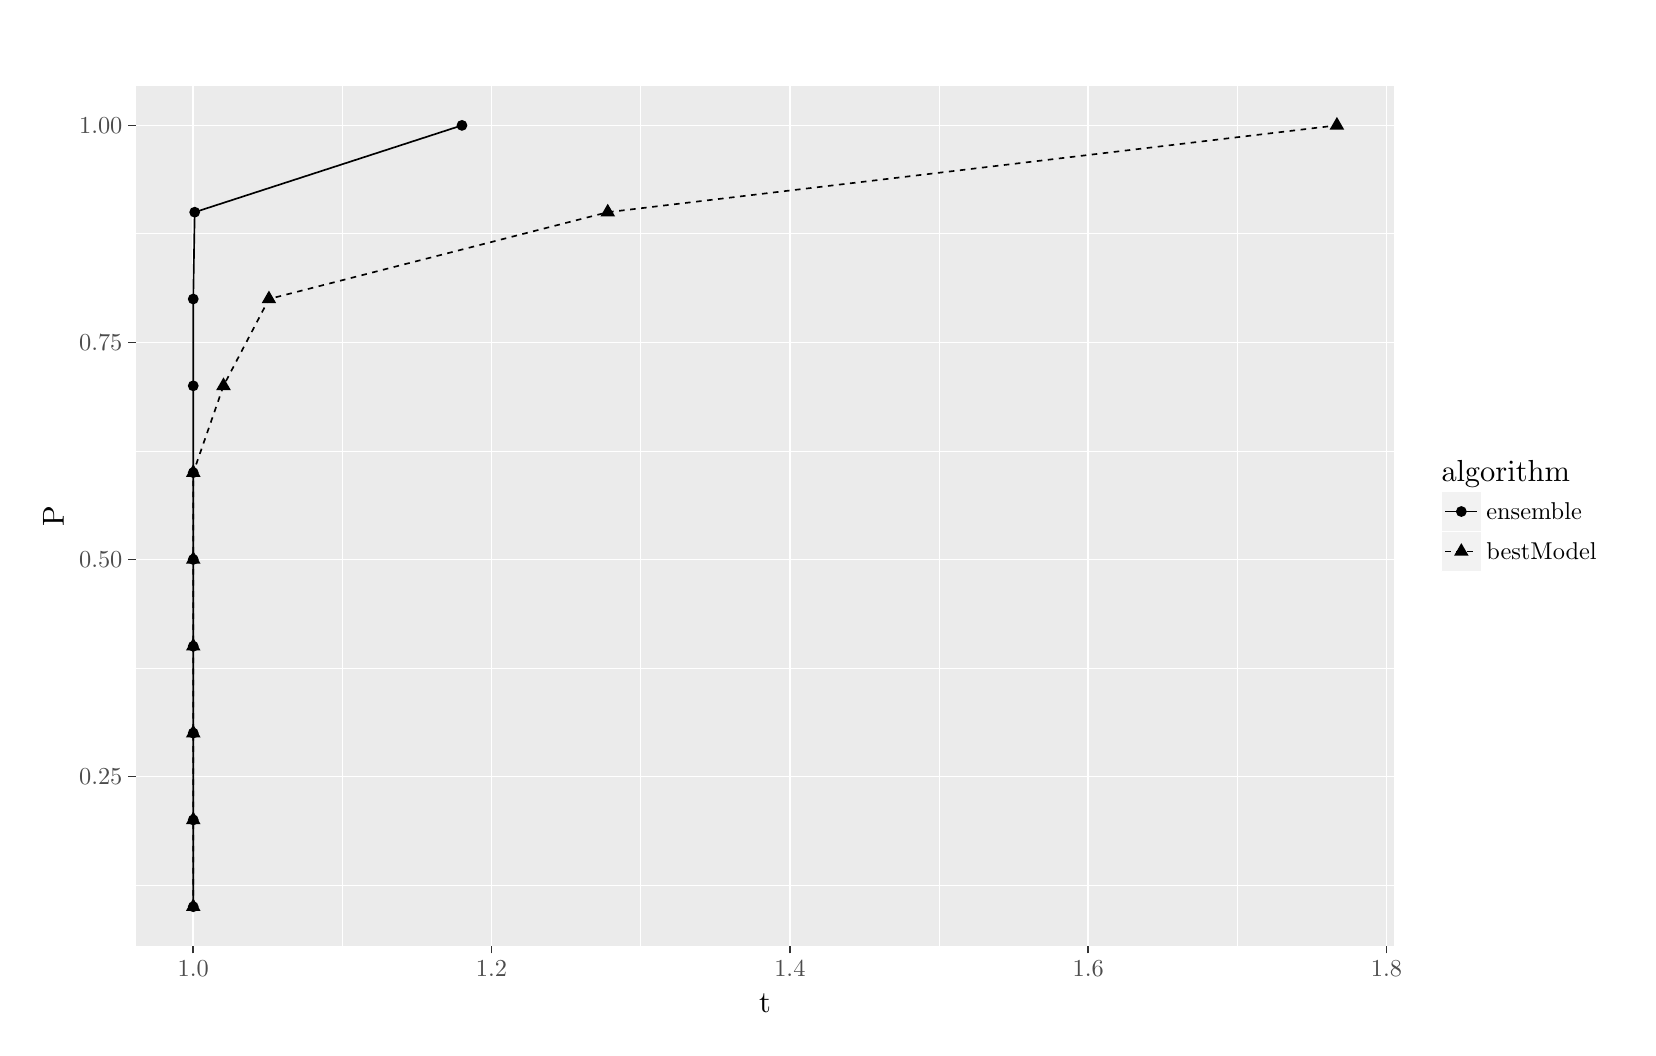
\begin{tikzpicture}[x=1pt,y=1pt]
\definecolor{fillColor}{RGB}{255,255,255}
\path[use as bounding box,fill=fillColor,fill opacity=0.00] (0,0) rectangle (578.16,361.35);
\begin{scope}
\path[clip] (  0.00,  0.00) rectangle (578.16,361.35);
\definecolor{drawColor}{RGB}{255,255,255}
\definecolor{fillColor}{RGB}{255,255,255}

\path[draw=drawColor,line width= 0.6pt,line join=round,line cap=round,fill=fillColor] (  0.00, -0.00) rectangle (578.16,361.35);
\end{scope}
\begin{scope}
\path[clip] ( 39.17, 29.59) rectangle (493.75,340.16);
\definecolor{fillColor}{gray}{0.92}

\path[fill=fillColor] ( 39.17, 29.59) rectangle (493.75,340.16);
\definecolor{drawColor}{RGB}{255,255,255}

\path[draw=drawColor,line width= 0.3pt,line join=round] ( 39.17, 51.55) --
	(493.75, 51.55);

\path[draw=drawColor,line width= 0.3pt,line join=round] ( 39.17,129.97) --
	(493.75,129.97);

\path[draw=drawColor,line width= 0.3pt,line join=round] ( 39.17,208.40) --
	(493.75,208.40);

\path[draw=drawColor,line width= 0.3pt,line join=round] ( 39.17,286.83) --
	(493.75,286.83);

\path[draw=drawColor,line width= 0.3pt,line join=round] (113.73, 29.59) --
	(113.73,340.16);

\path[draw=drawColor,line width= 0.3pt,line join=round] (221.52, 29.59) --
	(221.52,340.16);

\path[draw=drawColor,line width= 0.3pt,line join=round] (329.31, 29.59) --
	(329.31,340.16);

\path[draw=drawColor,line width= 0.3pt,line join=round] (437.11, 29.59) --
	(437.11,340.16);

\path[draw=drawColor,line width= 0.6pt,line join=round] ( 39.17, 90.76) --
	(493.75, 90.76);

\path[draw=drawColor,line width= 0.6pt,line join=round] ( 39.17,169.19) --
	(493.75,169.19);

\path[draw=drawColor,line width= 0.6pt,line join=round] ( 39.17,247.61) --
	(493.75,247.61);

\path[draw=drawColor,line width= 0.6pt,line join=round] ( 39.17,326.04) --
	(493.75,326.04);

\path[draw=drawColor,line width= 0.6pt,line join=round] ( 59.83, 29.59) --
	( 59.83,340.16);

\path[draw=drawColor,line width= 0.6pt,line join=round] (167.62, 29.59) --
	(167.62,340.16);

\path[draw=drawColor,line width= 0.6pt,line join=round] (275.42, 29.59) --
	(275.42,340.16);

\path[draw=drawColor,line width= 0.6pt,line join=round] (383.21, 29.59) --
	(383.21,340.16);

\path[draw=drawColor,line width= 0.6pt,line join=round] (491.00, 29.59) --
	(491.00,340.16);
\definecolor{drawColor}{RGB}{0,0,0}

\path[draw=drawColor,line width= 0.6pt,line join=round] ( 59.83, 43.70) --
	( 59.83, 75.07) --
	( 59.83,106.45) --
	( 59.83,137.82) --
	( 59.83,169.19) --
	( 59.83,200.56) --
	( 59.83,231.93) --
	( 59.83,263.30) --
	( 60.35,294.67) --
	(156.93,326.04);

\path[draw=drawColor,line width= 0.6pt,dash pattern=on 2pt off 2pt ,line join=round] ( 59.83, 43.70) --
	( 59.83, 75.07) --
	( 59.83,106.45) --
	( 59.83,137.82) --
	( 59.83,169.19) --
	( 59.84,200.56) --
	( 70.76,231.93) --
	( 87.18,263.30) --
	(209.61,294.67) --
	(473.09,326.04);
\definecolor{fillColor}{RGB}{0,0,0}

\path[fill=fillColor] ( 59.83, 43.70) circle (  1.96);

\path[fill=fillColor] ( 59.83, 75.07) circle (  1.96);

\path[fill=fillColor] ( 59.83,106.45) circle (  1.96);

\path[fill=fillColor] ( 59.83,137.82) circle (  1.96);

\path[fill=fillColor] ( 59.83,169.19) circle (  1.96);

\path[fill=fillColor] ( 59.83,200.56) circle (  1.96);

\path[fill=fillColor] ( 59.83,231.93) circle (  1.96);

\path[fill=fillColor] ( 59.83,263.30) circle (  1.96);

\path[fill=fillColor] ( 60.35,294.67) circle (  1.96);

\path[fill=fillColor] (156.93,326.04) circle (  1.96);

\path[fill=fillColor] ( 59.83, 46.75) --
	( 62.47, 42.18) --
	( 57.19, 42.18) --
	cycle;

\path[fill=fillColor] ( 59.83, 78.13) --
	( 62.47, 73.55) --
	( 57.19, 73.55) --
	cycle;

\path[fill=fillColor] ( 59.83,109.50) --
	( 62.47,104.92) --
	( 57.19,104.92) --
	cycle;

\path[fill=fillColor] ( 59.83,140.87) --
	( 62.47,136.29) --
	( 57.19,136.29) --
	cycle;

\path[fill=fillColor] ( 59.83,172.24) --
	( 62.47,167.66) --
	( 57.19,167.66) --
	cycle;

\path[fill=fillColor] ( 59.84,203.61) --
	( 62.48,199.03) --
	( 57.19,199.03) --
	cycle;

\path[fill=fillColor] ( 70.76,234.98) --
	( 73.40,230.40) --
	( 68.12,230.40) --
	cycle;

\path[fill=fillColor] ( 87.18,266.35) --
	( 89.82,261.77) --
	( 84.54,261.77) --
	cycle;

\path[fill=fillColor] (209.61,297.72) --
	(212.26,293.15) --
	(206.97,293.15) --
	cycle;

\path[fill=fillColor] (473.09,329.09) --
	(475.73,324.52) --
	(470.45,324.52) --
	cycle;
\end{scope}
\begin{scope}
\path[clip] (  0.00,  0.00) rectangle (578.16,361.35);
\definecolor{drawColor}{gray}{0.30}

\node[text=drawColor,anchor=base east,inner sep=0pt, outer sep=0pt, scale=  0.88] at ( 34.22, 87.73) {0.25};

\node[text=drawColor,anchor=base east,inner sep=0pt, outer sep=0pt, scale=  0.88] at ( 34.22,166.16) {0.50};

\node[text=drawColor,anchor=base east,inner sep=0pt, outer sep=0pt, scale=  0.88] at ( 34.22,244.58) {0.75};

\node[text=drawColor,anchor=base east,inner sep=0pt, outer sep=0pt, scale=  0.88] at ( 34.22,323.01) {1.00};
\end{scope}
\begin{scope}
\path[clip] (  0.00,  0.00) rectangle (578.16,361.35);
\definecolor{drawColor}{gray}{0.20}

\path[draw=drawColor,line width= 0.6pt,line join=round] ( 36.42, 90.76) --
	( 39.17, 90.76);

\path[draw=drawColor,line width= 0.6pt,line join=round] ( 36.42,169.19) --
	( 39.17,169.19);

\path[draw=drawColor,line width= 0.6pt,line join=round] ( 36.42,247.61) --
	( 39.17,247.61);

\path[draw=drawColor,line width= 0.6pt,line join=round] ( 36.42,326.04) --
	( 39.17,326.04);
\end{scope}
\begin{scope}
\path[clip] (  0.00,  0.00) rectangle (578.16,361.35);
\definecolor{drawColor}{gray}{0.20}

\path[draw=drawColor,line width= 0.6pt,line join=round] ( 59.83, 26.84) --
	( 59.83, 29.59);

\path[draw=drawColor,line width= 0.6pt,line join=round] (167.62, 26.84) --
	(167.62, 29.59);

\path[draw=drawColor,line width= 0.6pt,line join=round] (275.42, 26.84) --
	(275.42, 29.59);

\path[draw=drawColor,line width= 0.6pt,line join=round] (383.21, 26.84) --
	(383.21, 29.59);

\path[draw=drawColor,line width= 0.6pt,line join=round] (491.00, 26.84) --
	(491.00, 29.59);
\end{scope}
\begin{scope}
\path[clip] (  0.00,  0.00) rectangle (578.16,361.35);
\definecolor{drawColor}{gray}{0.30}

\node[text=drawColor,anchor=base,inner sep=0pt, outer sep=0pt, scale=  0.88] at ( 59.83, 18.58) {1.0};

\node[text=drawColor,anchor=base,inner sep=0pt, outer sep=0pt, scale=  0.88] at (167.62, 18.58) {1.2};

\node[text=drawColor,anchor=base,inner sep=0pt, outer sep=0pt, scale=  0.88] at (275.42, 18.58) {1.4};

\node[text=drawColor,anchor=base,inner sep=0pt, outer sep=0pt, scale=  0.88] at (383.21, 18.58) {1.6};

\node[text=drawColor,anchor=base,inner sep=0pt, outer sep=0pt, scale=  0.88] at (491.00, 18.58) {1.8};
\end{scope}
\begin{scope}
\path[clip] (  0.00,  0.00) rectangle (578.16,361.35);
\definecolor{drawColor}{RGB}{0,0,0}

\node[text=drawColor,anchor=base,inner sep=0pt, outer sep=0pt, scale=  1.10] at (266.46,  5.50) {t};
\end{scope}
\begin{scope}
\path[clip] (  0.00,  0.00) rectangle (578.16,361.35);
\definecolor{drawColor}{RGB}{0,0,0}

\node[text=drawColor,rotate= 90.00,anchor=base,inner sep=0pt, outer sep=0pt, scale=  1.10] at ( 13.08,184.87) {P};
\end{scope}
\begin{scope}
\path[clip] (  0.00,  0.00) rectangle (578.16,361.35);
\definecolor{fillColor}{RGB}{255,255,255}

\path[fill=fillColor] (505.13,159.13) rectangle (572.66,210.61);
\end{scope}
\begin{scope}
\path[clip] (  0.00,  0.00) rectangle (578.16,361.35);
\definecolor{drawColor}{RGB}{0,0,0}

\node[text=drawColor,anchor=base west,inner sep=0pt, outer sep=0pt, scale=  1.10] at (510.82,197.35) {algorithm};
\end{scope}
\begin{scope}
\path[clip] (  0.00,  0.00) rectangle (578.16,361.35);
\definecolor{drawColor}{RGB}{255,255,255}
\definecolor{fillColor}{gray}{0.95}

\path[draw=drawColor,line width= 0.6pt,line join=round,line cap=round,fill=fillColor] (510.82,179.28) rectangle (525.28,193.73);
\end{scope}
\begin{scope}
\path[clip] (  0.00,  0.00) rectangle (578.16,361.35);
\definecolor{drawColor}{RGB}{0,0,0}

\path[draw=drawColor,line width= 0.6pt,line join=round] (512.27,186.51) -- (523.83,186.51);
\end{scope}
\begin{scope}
\path[clip] (  0.00,  0.00) rectangle (578.16,361.35);
\definecolor{fillColor}{RGB}{0,0,0}

\path[fill=fillColor] (518.05,186.51) circle (  1.96);
\end{scope}
\begin{scope}
\path[clip] (  0.00,  0.00) rectangle (578.16,361.35);
\definecolor{drawColor}{RGB}{255,255,255}
\definecolor{fillColor}{gray}{0.95}

\path[draw=drawColor,line width= 0.6pt,line join=round,line cap=round,fill=fillColor] (510.82,164.82) rectangle (525.28,179.28);
\end{scope}
\begin{scope}
\path[clip] (  0.00,  0.00) rectangle (578.16,361.35);
\definecolor{drawColor}{RGB}{0,0,0}

\path[draw=drawColor,line width= 0.6pt,dash pattern=on 2pt off 2pt ,line join=round] (512.27,172.05) -- (523.83,172.05);
\end{scope}
\begin{scope}
\path[clip] (  0.00,  0.00) rectangle (578.16,361.35);
\definecolor{fillColor}{RGB}{0,0,0}

\path[fill=fillColor] (518.05,175.10) --
	(520.69,170.53) --
	(515.41,170.53) --
	cycle;
\end{scope}
\begin{scope}
\path[clip] (  0.00,  0.00) rectangle (578.16,361.35);
\definecolor{drawColor}{RGB}{0,0,0}

\node[text=drawColor,anchor=base west,inner sep=0pt, outer sep=0pt, scale=  0.88] at (527.09,183.47) {ensemble};
\end{scope}
\begin{scope}
\path[clip] (  0.00,  0.00) rectangle (578.16,361.35);
\definecolor{drawColor}{RGB}{0,0,0}

\node[text=drawColor,anchor=base west,inner sep=0pt, outer sep=0pt, scale=  0.88] at (527.09,169.02) {bestModel};
\end{scope}
\end{tikzpicture}

}
		\caption[Διάγραμμα προφίλ απόδοσης για τη σύγκριση του ensemble με το βέλτιστο μοντέλο]{Διάγραμμα προφίλ απόδοσης για τη σύγκριση του ensemble με το βέλτιστο μοντέλο: Παρατηρούμε πως o ensemble υπερισχύει του βέλτιστου μοντέλου σε όλα τα σετ δεδομένων. }
		\label{fig:ensprof}
\end{figure}

Η εφαρμογή του Wilcoxon rank-sum τεστ με επίπεδο εμπιστοσύνης $95\%$, εφαρμογή διόρθωσης συνέχειας (Παράρτημα \ref{appendix:Tests}) και συνυπολογισμό του ότι τα πειράματα είναι ζευγαρωμένα (paired) δίνει p-value 0.8336.  

\paragraph{Συμπεράσματα}
Το διάγραμμα απόδοσης του Σχήματος \ref{fig:ensprof} και το στατιστικό τεστ που εφαρμόσαμε συμφωνούν ότι ο ensemble έχει απόδοση ισότιμη του καλύτερου μοντέλου της βιβλιοθήκης και δεν υπάρχει στατιστικά σημαντική διαφορά μεταξύ τους. Το διάγραμμα απόδοσης επίσης δίνει μεγαλύτερη πιθανότητα στον ensemble να έχει απόδοση πλησιέστερη στη βέλτιστη.
 
\section{Αξιολόγηση συστήματος Automated Data Scientist}\label{section:eval_system}
Η αξιολόγηση του Automated Data Scientist στοχεύει να αποδείξει ότι το σύστημα που έχουμε σχεδιάσει έχει απόδοση συγκρίσιμη με τεχνικές της σύγχρονης βιβλιογραφίας. Καθώς η ουσιαστική πρωτοτυπία του συστήματος βρίσκεται στον τρόπο με τον οποίο γίνεται η βελτιστοποίηση των υπερ-παρα\-μέ\-τρων για τα μοντέλα μηχανικής μάθησης που χρησιμοποιούμε θα συγκρίνουμε το σύστημά μας με δύο τεχνικές βελτιστοποίησης:
\begin{itemize}
	\item \textbf{πλεγματική αναζήτηση} Πρόκειται για τη συνηθέστερη τεχνική αναζήτησης υπερπαρα\-μέτρων μέχρι και σήμερα.
	\item \textbf{Tree Parzen Estimator} Η τεχνική αυτή, που έχει περιγραφεί στην ενότητα \ref{section:SMBO} αποτελεί state of the art στο χώρο του AutoML.
\end{itemize}

Eπίσης, προκειμένου να αξιολογηθεί η συνεισφορά της τεχνικής σχηματισμού ensemble  με προς-τα-εμπρός επιλογής μοντέλων πραγματοποιούμε 4 διαφορετικά πειράματα: ένα για κάθε αλγόριθμο μάθησης, όπου εκπαιδεύονται μοντέλα μόνο με το συγκεκριμένο και ένα συνολικό, όπου ο ensemble χρησιμοποιεί όλους τους αλγορίθμους. 

Για την αξιολόγηση του συστήματος θα χρησιμοποιηθούν δύο τεχνικές της σύγχρονης βιβλιογραφίας: στατισικά τεστ για τη διαπίστωση σημαντικής διαφοράς στην απόδοση των αλγορίθμων και διαγράμματα προφίλ απόδοσης για την οπτικοποίηση της απόδοσης των αλγορίθμων στα διαφορετικά σετ δεδομένων. 

Εφαρμόζωντας το στατιστικό τεστ Friedman rank sum για σύγκριση μεταξύ πολλαπλών αλγορίθμων διαπιστώνουμε σημαντική στατιστική διαφορά καθώς το p-value είναι $6.285 \cdot 10^{-5}$ για επίπεδο εμπιστοσύνης $0.95$. Προκειμένου να εντοπίσουμε τα ζεύγη των αλγορίθμων τα οποία προκαλούν τη σημαντική στατιστική διαφορά θα εφαρμόσουμε το Nemenyi post-hoc τεστ.

	\begin{table}[!htb]
		\begin{center}
			\caption[Στατιστικό τεστ απόδοσης συνολικού συστήματος]{Ο πίνακας αυτός περιέχει τα p-values του post-hoc Nemenyi τεστ για τη διαπίστωση στατιστικής διαφοράς μεταξύ των διαφορετικών μεθόδων ανά ζεύγη. Το τεστ αυτό εφαρμόστηκε μετά από τη διαπίστωση στατιστικής διαφοράς με το Friedman rank sum τεστ. Με έντονη γραφή παρουσιάζονται τα ζεύγη τα οποία εμφανίζουν στατιστικά σημαντική διαφορά.}
			\label{table:pvalues}
			\scalebox{0.8}{
			\begin{tabular}{ |c|c|c|c|c|c|c|c|c| } 
				\hline
				&automl & ensembleGrid & ensembleTpe & knnGrid & nknnTpe & nnetGrid & nnetTpe & treeGrid\\
				\hline
			    ensembleGrid & $\bm{0.0021}$ &  ---  &  ---  &  ---  & ---  & ---  & ---  & ---  \\
			    ensembleTpe & $\bm{0.0021}$ & 1 & ---  & ---  & ---  & ---  & ---  & --- \\
			    knnGrid & 0.9213 & 0.1593 & 0.1593 &  --- &  --- & ---  & ---  & ---  \\
			    knnTpe & 0.9213 & 0.1593 & 0.1593& 1 &  --- & ---  & ---  &  --- \\
			    nnetGrid & 0.2337 & 0.8531 & 0.8531 & 0.9643& 0.9643 &- & --- & --- \\
			    nnetTpe & 0.7854 & 0.3024 & 0.3024 & 1 & 1 & 0.9949 & ---  & --- \\
			    treeGrid & 0.8321 & 0.2554 & 0.2554 & 1 & 1 & 0.9902 & 1 & --- \\
			    treeTpe & 1 & $\bm{0.0067}$ & $\bm{0.0067}$ & 0.9828 & 0.9828 & 0.409 & 0.9213 & 0.9457 \\	    
				\hline
			\end{tabular}}
		\end{center}			
	\end{table} 


\begin{figure}[!htb]
	\scalebox{0.8}{
	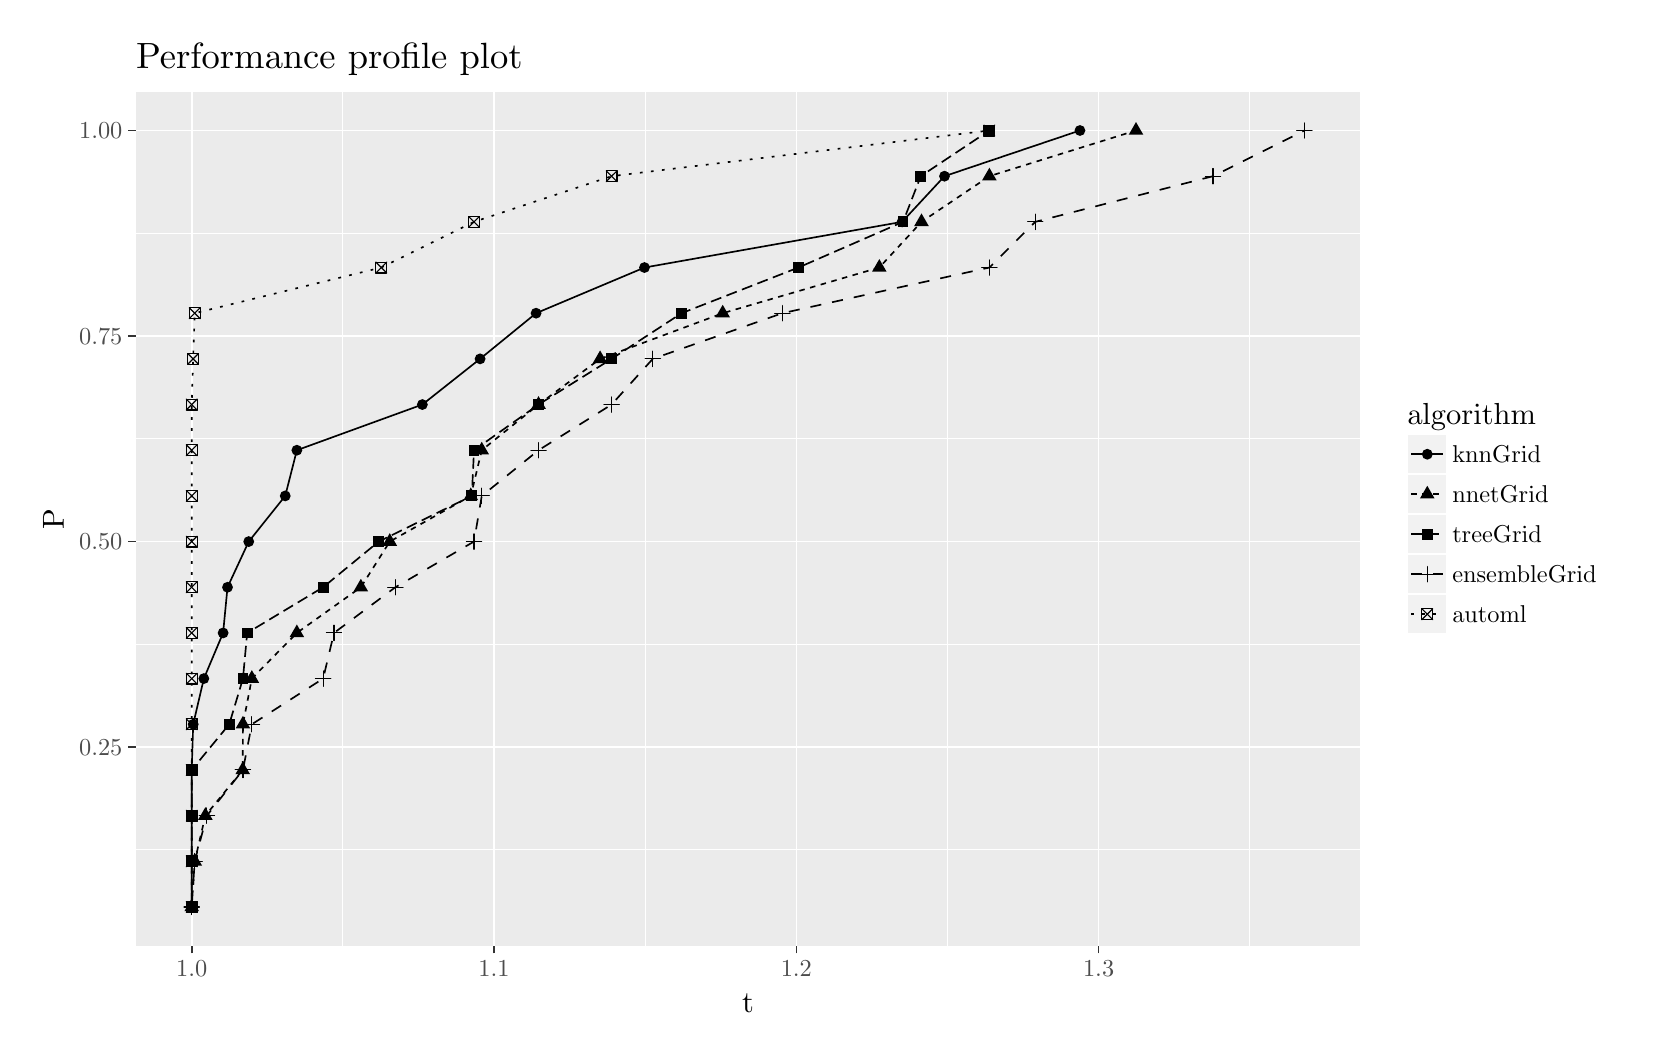
\begin{tikzpicture}[x=1pt,y=1pt]
\definecolor{fillColor}{RGB}{255,255,255}
\path[use as bounding box,fill=fillColor,fill opacity=0.00] (0,0) rectangle (578.16,361.35);
\begin{scope}
\path[clip] (  0.00,  0.00) rectangle (578.16,361.35);
\definecolor{drawColor}{RGB}{255,255,255}
\definecolor{fillColor}{RGB}{255,255,255}

\path[draw=drawColor,line width= 0.6pt,line join=round,line cap=round,fill=fillColor] (  0.00,  0.00) rectangle (578.16,361.35);
\end{scope}
\begin{scope}
\path[clip] ( 39.17, 29.59) rectangle (481.45,338.21);
\definecolor{fillColor}{gray}{0.92}

\path[fill=fillColor] ( 39.17, 29.59) rectangle (481.45,338.21);
\definecolor{drawColor}{RGB}{255,255,255}

\path[draw=drawColor,line width= 0.3pt,line join=round] ( 39.17, 64.25) --
	(481.45, 64.25);

\path[draw=drawColor,line width= 0.3pt,line join=round] ( 39.17,138.51) --
	(481.45,138.51);

\path[draw=drawColor,line width= 0.3pt,line join=round] ( 39.17,212.78) --
	(481.45,212.78);

\path[draw=drawColor,line width= 0.3pt,line join=round] ( 39.17,287.05) --
	(481.45,287.05);

\path[draw=drawColor,line width= 0.3pt,line join=round] (113.89, 29.59) --
	(113.89,338.21);

\path[draw=drawColor,line width= 0.3pt,line join=round] (223.13, 29.59) --
	(223.13,338.21);

\path[draw=drawColor,line width= 0.3pt,line join=round] (332.37, 29.59) --
	(332.37,338.21);

\path[draw=drawColor,line width= 0.3pt,line join=round] (441.61, 29.59) --
	(441.61,338.21);

\path[draw=drawColor,line width= 0.6pt,line join=round] ( 39.17,101.38) --
	(481.45,101.38);

\path[draw=drawColor,line width= 0.6pt,line join=round] ( 39.17,175.65) --
	(481.45,175.65);

\path[draw=drawColor,line width= 0.6pt,line join=round] ( 39.17,249.92) --
	(481.45,249.92);

\path[draw=drawColor,line width= 0.6pt,line join=round] ( 39.17,324.19) --
	(481.45,324.19);

\path[draw=drawColor,line width= 0.6pt,line join=round] ( 59.27, 29.59) --
	( 59.27,338.21);

\path[draw=drawColor,line width= 0.6pt,line join=round] (168.51, 29.59) --
	(168.51,338.21);

\path[draw=drawColor,line width= 0.6pt,line join=round] (277.75, 29.59) --
	(277.75,338.21);

\path[draw=drawColor,line width= 0.6pt,line join=round] (386.99, 29.59) --
	(386.99,338.21);
\definecolor{drawColor}{RGB}{0,0,0}

\path[draw=drawColor,line width= 0.6pt,line join=round] ( 59.27, 43.62) --
	( 59.27, 60.12) --
	( 59.27, 76.62) --
	( 59.27, 93.13) --
	( 59.81,109.63) --
	( 63.66,126.14) --
	( 70.62,142.64) --
	( 72.21,159.14) --
	( 79.88,175.65) --
	( 93.07,192.15) --
	( 97.27,208.66) --
	(142.62,225.16) --
	(163.48,241.67) --
	(183.71,258.17) --
	(222.88,274.67) --
	(315.97,291.18) --
	(331.29,307.68) --
	(380.23,324.19);

\path[draw=drawColor,line width= 0.6pt,dash pattern=on 2pt off 2pt ,line join=round] ( 59.27, 43.62) --
	( 60.36, 60.12) --
	( 64.21, 76.62) --
	( 77.71, 93.13) --
	( 77.79,109.63) --
	( 81.00,126.14) --
	( 97.27,142.64) --
	(120.40,159.14) --
	(130.84,175.65) --
	(160.12,192.15) --
	(164.08,208.66) --
	(184.60,225.16) --
	(206.85,241.67) --
	(251.15,258.17) --
	(307.74,274.67) --
	(322.98,291.18) --
	(347.51,307.68) --
	(400.49,324.19);

\path[draw=drawColor,line width= 0.6pt,dash pattern=on 4pt off 2pt ,line join=round] ( 59.27, 43.62) --
	( 59.27, 60.12) --
	( 59.27, 76.62) --
	( 59.27, 93.13) --
	( 72.83,109.63) --
	( 77.79,126.14) --
	( 79.32,142.64) --
	(106.77,159.14) --
	(126.84,175.65) --
	(160.49,192.15) --
	(161.28,208.66) --
	(184.60,225.16) --
	(211.00,241.67) --
	(236.29,258.17) --
	(278.51,274.67) --
	(316.32,291.18) --
	(322.71,307.68) --
	(347.51,324.19);

\path[draw=drawColor,line width= 0.6pt,dash pattern=on 4pt off 4pt ,line join=round] ( 59.27, 43.62) --
	( 60.36, 60.12) --
	( 64.76, 76.62) --
	( 77.79, 93.13) --
	( 81.00,109.63) --
	(106.77,126.14) --
	(110.69,142.64) --
	(132.86,159.14) --
	(161.28,175.65) --
	(164.08,192.15) --
	(184.60,208.66) --
	(211.00,225.16) --
	(225.88,241.67) --
	(272.69,258.17) --
	(347.51,274.67) --
	(364.08,291.18) --
	(428.32,307.68) --
	(461.34,324.19);

\path[draw=drawColor,line width= 0.6pt,dash pattern=on 1pt off 3pt ,line join=round] ( 59.27, 43.62) --
	( 59.27, 60.12) --
	( 59.27, 76.62) --
	( 59.27, 93.13) --
	( 59.27,109.63) --
	( 59.27,126.14) --
	( 59.27,142.64) --
	( 59.27,159.14) --
	( 59.27,175.65) --
	( 59.27,192.15) --
	( 59.27,208.66) --
	( 59.27,225.16) --
	( 59.79,241.67) --
	( 60.36,258.17) --
	(127.77,274.67) --
	(161.28,291.18) --
	(211.00,307.68) --
	(347.51,324.19);
\definecolor{fillColor}{RGB}{0,0,0}

\path[fill=fillColor] ( 59.27, 43.62) circle (  1.96);

\path[fill=fillColor] ( 59.27, 60.12) circle (  1.96);

\path[fill=fillColor] ( 59.27, 76.62) circle (  1.96);

\path[fill=fillColor] ( 59.27, 93.13) circle (  1.96);

\path[fill=fillColor] ( 59.81,109.63) circle (  1.96);

\path[fill=fillColor] ( 63.66,126.14) circle (  1.96);

\path[fill=fillColor] ( 70.62,142.64) circle (  1.96);

\path[fill=fillColor] ( 72.21,159.14) circle (  1.96);

\path[fill=fillColor] ( 79.88,175.65) circle (  1.96);

\path[fill=fillColor] ( 93.07,192.15) circle (  1.96);

\path[fill=fillColor] ( 97.27,208.66) circle (  1.96);

\path[fill=fillColor] (142.62,225.16) circle (  1.96);

\path[fill=fillColor] (163.48,241.67) circle (  1.96);

\path[fill=fillColor] (183.71,258.17) circle (  1.96);

\path[fill=fillColor] (222.88,274.67) circle (  1.96);

\path[fill=fillColor] (315.97,291.18) circle (  1.96);

\path[fill=fillColor] (331.29,307.68) circle (  1.96);

\path[fill=fillColor] (380.23,324.19) circle (  1.96);

\path[fill=fillColor] ( 59.27, 46.67) --
	( 61.91, 42.09) --
	( 56.63, 42.09) --
	cycle;

\path[fill=fillColor] ( 60.36, 63.17) --
	( 63.00, 58.59) --
	( 57.72, 58.59) --
	cycle;

\path[fill=fillColor] ( 64.21, 79.67) --
	( 66.85, 75.10) --
	( 61.57, 75.10) --
	cycle;

\path[fill=fillColor] ( 77.71, 96.18) --
	( 80.35, 91.60) --
	( 75.07, 91.60) --
	cycle;

\path[fill=fillColor] ( 77.79,112.68) --
	( 80.43,108.11) --
	( 75.14,108.11) --
	cycle;

\path[fill=fillColor] ( 81.00,129.19) --
	( 83.64,124.61) --
	( 78.35,124.61) --
	cycle;

\path[fill=fillColor] ( 97.27,145.69) --
	( 99.91,141.11) --
	( 94.62,141.11) --
	cycle;

\path[fill=fillColor] (120.40,162.20) --
	(123.04,157.62) --
	(117.75,157.62) --
	cycle;

\path[fill=fillColor] (130.84,178.70) --
	(133.49,174.12) --
	(128.20,174.12) --
	cycle;

\path[fill=fillColor] (160.12,195.20) --
	(162.76,190.63) --
	(157.48,190.63) --
	cycle;

\path[fill=fillColor] (164.08,211.71) --
	(166.72,207.13) --
	(161.44,207.13) --
	cycle;

\path[fill=fillColor] (184.60,228.21) --
	(187.24,223.64) --
	(181.96,223.64) --
	cycle;

\path[fill=fillColor] (206.85,244.72) --
	(209.49,240.14) --
	(204.21,240.14) --
	cycle;

\path[fill=fillColor] (251.15,261.22) --
	(253.79,256.64) --
	(248.51,256.64) --
	cycle;

\path[fill=fillColor] (307.74,277.73) --
	(310.38,273.15) --
	(305.10,273.15) --
	cycle;

\path[fill=fillColor] (322.98,294.23) --
	(325.62,289.65) --
	(320.33,289.65) --
	cycle;

\path[fill=fillColor] (347.51,310.73) --
	(350.15,306.16) --
	(344.86,306.16) --
	cycle;

\path[fill=fillColor] (400.49,327.24) --
	(403.14,322.66) --
	(397.85,322.66) --
	cycle;

\path[fill=fillColor] ( 57.31, 41.65) --
	( 61.23, 41.65) --
	( 61.23, 45.58) --
	( 57.31, 45.58) --
	cycle;

\path[fill=fillColor] ( 57.31, 58.16) --
	( 61.23, 58.16) --
	( 61.23, 62.08) --
	( 57.31, 62.08) --
	cycle;

\path[fill=fillColor] ( 57.31, 74.66) --
	( 61.23, 74.66) --
	( 61.23, 78.59) --
	( 57.31, 78.59) --
	cycle;

\path[fill=fillColor] ( 57.31, 91.17) --
	( 61.23, 91.17) --
	( 61.23, 95.09) --
	( 57.31, 95.09) --
	cycle;

\path[fill=fillColor] ( 70.87,107.67) --
	( 74.79,107.67) --
	( 74.79,111.59) --
	( 70.87,111.59) --
	cycle;

\path[fill=fillColor] ( 75.82,124.17) --
	( 79.75,124.17) --
	( 79.75,128.10) --
	( 75.82,128.10) --
	cycle;

\path[fill=fillColor] ( 77.36,140.68) --
	( 81.29,140.68) --
	( 81.29,144.60) --
	( 77.36,144.60) --
	cycle;

\path[fill=fillColor] (104.80,157.18) --
	(108.73,157.18) --
	(108.73,161.11) --
	(104.80,161.11) --
	cycle;

\path[fill=fillColor] (124.87,173.69) --
	(128.80,173.69) --
	(128.80,177.61) --
	(124.87,177.61) --
	cycle;

\path[fill=fillColor] (158.53,190.19) --
	(162.45,190.19) --
	(162.45,194.12) --
	(158.53,194.12) --
	cycle;

\path[fill=fillColor] (159.32,206.69) --
	(163.24,206.69) --
	(163.24,210.62) --
	(159.32,210.62) --
	cycle;

\path[fill=fillColor] (182.64,223.20) --
	(186.56,223.20) --
	(186.56,227.12) --
	(182.64,227.12) --
	cycle;

\path[fill=fillColor] (209.03,239.70) --
	(212.96,239.70) --
	(212.96,243.63) --
	(209.03,243.63) --
	cycle;

\path[fill=fillColor] (234.33,256.21) --
	(238.25,256.21) --
	(238.25,260.13) --
	(234.33,260.13) --
	cycle;

\path[fill=fillColor] (276.54,272.71) --
	(280.47,272.71) --
	(280.47,276.64) --
	(276.54,276.64) --
	cycle;

\path[fill=fillColor] (314.36,289.22) --
	(318.28,289.22) --
	(318.28,293.14) --
	(314.36,293.14) --
	cycle;

\path[fill=fillColor] (320.75,305.72) --
	(324.67,305.72) --
	(324.67,309.64) --
	(320.75,309.64) --
	cycle;

\path[fill=fillColor] (345.54,322.22) --
	(349.47,322.22) --
	(349.47,326.15) --
	(345.54,326.15) --
	cycle;

\path[draw=drawColor,line width= 0.4pt,line join=round,line cap=round] ( 56.50, 43.62) -- ( 62.05, 43.62);

\path[draw=drawColor,line width= 0.4pt,line join=round,line cap=round] ( 59.27, 40.84) -- ( 59.27, 46.39);

\path[draw=drawColor,line width= 0.4pt,line join=round,line cap=round] ( 57.59, 60.12) -- ( 63.14, 60.12);

\path[draw=drawColor,line width= 0.4pt,line join=round,line cap=round] ( 60.36, 57.34) -- ( 60.36, 62.89);

\path[draw=drawColor,line width= 0.4pt,line join=round,line cap=round] ( 61.98, 76.62) -- ( 67.53, 76.62);

\path[draw=drawColor,line width= 0.4pt,line join=round,line cap=round] ( 64.76, 73.85) -- ( 64.76, 79.40);

\path[draw=drawColor,line width= 0.4pt,line join=round,line cap=round] ( 75.01, 93.13) -- ( 80.56, 93.13);

\path[draw=drawColor,line width= 0.4pt,line join=round,line cap=round] ( 77.79, 90.35) -- ( 77.79, 95.90);

\path[draw=drawColor,line width= 0.4pt,line join=round,line cap=round] ( 78.22,109.63) -- ( 83.77,109.63);

\path[draw=drawColor,line width= 0.4pt,line join=round,line cap=round] ( 81.00,106.86) -- ( 81.00,112.41);

\path[draw=drawColor,line width= 0.4pt,line join=round,line cap=round] (103.99,126.14) -- (109.54,126.14);

\path[draw=drawColor,line width= 0.4pt,line join=round,line cap=round] (106.77,123.36) -- (106.77,128.91);

\path[draw=drawColor,line width= 0.4pt,line join=round,line cap=round] (107.91,142.64) -- (113.46,142.64);

\path[draw=drawColor,line width= 0.4pt,line join=round,line cap=round] (110.69,139.87) -- (110.69,145.42);

\path[draw=drawColor,line width= 0.4pt,line join=round,line cap=round] (130.09,159.14) -- (135.64,159.14);

\path[draw=drawColor,line width= 0.4pt,line join=round,line cap=round] (132.86,156.37) -- (132.86,161.92);

\path[draw=drawColor,line width= 0.4pt,line join=round,line cap=round] (158.51,175.65) -- (164.06,175.65);

\path[draw=drawColor,line width= 0.4pt,line join=round,line cap=round] (161.28,172.87) -- (161.28,178.42);

\path[draw=drawColor,line width= 0.4pt,line join=round,line cap=round] (161.30,192.15) -- (166.85,192.15);

\path[draw=drawColor,line width= 0.4pt,line join=round,line cap=round] (164.08,189.38) -- (164.08,194.93);

\path[draw=drawColor,line width= 0.4pt,line join=round,line cap=round] (181.82,208.66) -- (187.37,208.66);

\path[draw=drawColor,line width= 0.4pt,line join=round,line cap=round] (184.60,205.88) -- (184.60,211.43);

\path[draw=drawColor,line width= 0.4pt,line join=round,line cap=round] (208.22,225.16) -- (213.77,225.16);

\path[draw=drawColor,line width= 0.4pt,line join=round,line cap=round] (211.00,222.39) -- (211.00,227.94);

\path[draw=drawColor,line width= 0.4pt,line join=round,line cap=round] (223.11,241.67) -- (228.66,241.67);

\path[draw=drawColor,line width= 0.4pt,line join=round,line cap=round] (225.88,238.89) -- (225.88,244.44);

\path[draw=drawColor,line width= 0.4pt,line join=round,line cap=round] (269.92,258.17) -- (275.47,258.17);

\path[draw=drawColor,line width= 0.4pt,line join=round,line cap=round] (272.69,255.39) -- (272.69,260.94);

\path[draw=drawColor,line width= 0.4pt,line join=round,line cap=round] (344.73,274.67) -- (350.28,274.67);

\path[draw=drawColor,line width= 0.4pt,line join=round,line cap=round] (347.51,271.90) -- (347.51,277.45);

\path[draw=drawColor,line width= 0.4pt,line join=round,line cap=round] (361.31,291.18) -- (366.86,291.18);

\path[draw=drawColor,line width= 0.4pt,line join=round,line cap=round] (364.08,288.40) -- (364.08,293.95);

\path[draw=drawColor,line width= 0.4pt,line join=round,line cap=round] (425.55,307.68) -- (431.09,307.68);

\path[draw=drawColor,line width= 0.4pt,line join=round,line cap=round] (428.32,304.91) -- (428.32,310.46);

\path[draw=drawColor,line width= 0.4pt,line join=round,line cap=round] (458.57,324.19) -- (464.12,324.19);

\path[draw=drawColor,line width= 0.4pt,line join=round,line cap=round] (461.34,321.41) -- (461.34,326.96);

\path[draw=drawColor,line width= 0.4pt,line join=round,line cap=round] ( 57.31, 41.65) rectangle ( 61.23, 45.58);

\path[draw=drawColor,line width= 0.4pt,line join=round,line cap=round] ( 57.31, 41.65) -- ( 61.23, 45.58);

\path[draw=drawColor,line width= 0.4pt,line join=round,line cap=round] ( 57.31, 45.58) -- ( 61.23, 41.65);

\path[draw=drawColor,line width= 0.4pt,line join=round,line cap=round] ( 57.31, 58.16) rectangle ( 61.23, 62.08);

\path[draw=drawColor,line width= 0.4pt,line join=round,line cap=round] ( 57.31, 58.16) -- ( 61.23, 62.08);

\path[draw=drawColor,line width= 0.4pt,line join=round,line cap=round] ( 57.31, 62.08) -- ( 61.23, 58.16);

\path[draw=drawColor,line width= 0.4pt,line join=round,line cap=round] ( 57.31, 74.66) rectangle ( 61.23, 78.59);

\path[draw=drawColor,line width= 0.4pt,line join=round,line cap=round] ( 57.31, 74.66) -- ( 61.23, 78.59);

\path[draw=drawColor,line width= 0.4pt,line join=round,line cap=round] ( 57.31, 78.59) -- ( 61.23, 74.66);

\path[draw=drawColor,line width= 0.4pt,line join=round,line cap=round] ( 57.31, 91.17) rectangle ( 61.23, 95.09);

\path[draw=drawColor,line width= 0.4pt,line join=round,line cap=round] ( 57.31, 91.17) -- ( 61.23, 95.09);

\path[draw=drawColor,line width= 0.4pt,line join=round,line cap=round] ( 57.31, 95.09) -- ( 61.23, 91.17);

\path[draw=drawColor,line width= 0.4pt,line join=round,line cap=round] ( 57.31,107.67) rectangle ( 61.23,111.59);

\path[draw=drawColor,line width= 0.4pt,line join=round,line cap=round] ( 57.31,107.67) -- ( 61.23,111.59);

\path[draw=drawColor,line width= 0.4pt,line join=round,line cap=round] ( 57.31,111.59) -- ( 61.23,107.67);

\path[draw=drawColor,line width= 0.4pt,line join=round,line cap=round] ( 57.31,124.17) rectangle ( 61.23,128.10);

\path[draw=drawColor,line width= 0.4pt,line join=round,line cap=round] ( 57.31,124.17) -- ( 61.23,128.10);

\path[draw=drawColor,line width= 0.4pt,line join=round,line cap=round] ( 57.31,128.10) -- ( 61.23,124.17);

\path[draw=drawColor,line width= 0.4pt,line join=round,line cap=round] ( 57.31,140.68) rectangle ( 61.23,144.60);

\path[draw=drawColor,line width= 0.4pt,line join=round,line cap=round] ( 57.31,140.68) -- ( 61.23,144.60);

\path[draw=drawColor,line width= 0.4pt,line join=round,line cap=round] ( 57.31,144.60) -- ( 61.23,140.68);

\path[draw=drawColor,line width= 0.4pt,line join=round,line cap=round] ( 57.31,157.18) rectangle ( 61.23,161.11);

\path[draw=drawColor,line width= 0.4pt,line join=round,line cap=round] ( 57.31,157.18) -- ( 61.23,161.11);

\path[draw=drawColor,line width= 0.4pt,line join=round,line cap=round] ( 57.31,161.11) -- ( 61.23,157.18);

\path[draw=drawColor,line width= 0.4pt,line join=round,line cap=round] ( 57.31,173.69) rectangle ( 61.23,177.61);

\path[draw=drawColor,line width= 0.4pt,line join=round,line cap=round] ( 57.31,173.69) -- ( 61.23,177.61);

\path[draw=drawColor,line width= 0.4pt,line join=round,line cap=round] ( 57.31,177.61) -- ( 61.23,173.69);

\path[draw=drawColor,line width= 0.4pt,line join=round,line cap=round] ( 57.31,190.19) rectangle ( 61.23,194.12);

\path[draw=drawColor,line width= 0.4pt,line join=round,line cap=round] ( 57.31,190.19) -- ( 61.23,194.12);

\path[draw=drawColor,line width= 0.4pt,line join=round,line cap=round] ( 57.31,194.12) -- ( 61.23,190.19);

\path[draw=drawColor,line width= 0.4pt,line join=round,line cap=round] ( 57.31,206.69) rectangle ( 61.23,210.62);

\path[draw=drawColor,line width= 0.4pt,line join=round,line cap=round] ( 57.31,206.69) -- ( 61.23,210.62);

\path[draw=drawColor,line width= 0.4pt,line join=round,line cap=round] ( 57.31,210.62) -- ( 61.23,206.69);

\path[draw=drawColor,line width= 0.4pt,line join=round,line cap=round] ( 57.31,223.20) rectangle ( 61.23,227.12);

\path[draw=drawColor,line width= 0.4pt,line join=round,line cap=round] ( 57.31,223.20) -- ( 61.23,227.12);

\path[draw=drawColor,line width= 0.4pt,line join=round,line cap=round] ( 57.31,227.12) -- ( 61.23,223.20);

\path[draw=drawColor,line width= 0.4pt,line join=round,line cap=round] ( 57.83,239.70) rectangle ( 61.75,243.63);

\path[draw=drawColor,line width= 0.4pt,line join=round,line cap=round] ( 57.83,239.70) -- ( 61.75,243.63);

\path[draw=drawColor,line width= 0.4pt,line join=round,line cap=round] ( 57.83,243.63) -- ( 61.75,239.70);

\path[draw=drawColor,line width= 0.4pt,line join=round,line cap=round] ( 58.40,256.21) rectangle ( 62.32,260.13);

\path[draw=drawColor,line width= 0.4pt,line join=round,line cap=round] ( 58.40,256.21) -- ( 62.32,260.13);

\path[draw=drawColor,line width= 0.4pt,line join=round,line cap=round] ( 58.40,260.13) -- ( 62.32,256.21);

\path[draw=drawColor,line width= 0.4pt,line join=round,line cap=round] (125.81,272.71) rectangle (129.73,276.64);

\path[draw=drawColor,line width= 0.4pt,line join=round,line cap=round] (125.81,272.71) -- (129.73,276.64);

\path[draw=drawColor,line width= 0.4pt,line join=round,line cap=round] (125.81,276.64) -- (129.73,272.71);

\path[draw=drawColor,line width= 0.4pt,line join=round,line cap=round] (159.32,289.22) rectangle (163.24,293.14);

\path[draw=drawColor,line width= 0.4pt,line join=round,line cap=round] (159.32,289.22) -- (163.24,293.14);

\path[draw=drawColor,line width= 0.4pt,line join=round,line cap=round] (159.32,293.14) -- (163.24,289.22);

\path[draw=drawColor,line width= 0.4pt,line join=round,line cap=round] (209.03,305.72) rectangle (212.96,309.64);

\path[draw=drawColor,line width= 0.4pt,line join=round,line cap=round] (209.03,305.72) -- (212.96,309.64);

\path[draw=drawColor,line width= 0.4pt,line join=round,line cap=round] (209.03,309.64) -- (212.96,305.72);

\path[draw=drawColor,line width= 0.4pt,line join=round,line cap=round] (345.54,322.22) rectangle (349.47,326.15);

\path[draw=drawColor,line width= 0.4pt,line join=round,line cap=round] (345.54,322.22) -- (349.47,326.15);

\path[draw=drawColor,line width= 0.4pt,line join=round,line cap=round] (345.54,326.15) -- (349.47,322.22);
\end{scope}
\begin{scope}
\path[clip] (  0.00,  0.00) rectangle (578.16,361.35);
\definecolor{drawColor}{gray}{0.30}

\node[text=drawColor,anchor=base east,inner sep=0pt, outer sep=0pt, scale=  0.88] at ( 34.22, 98.35) {0.25};

\node[text=drawColor,anchor=base east,inner sep=0pt, outer sep=0pt, scale=  0.88] at ( 34.22,172.62) {0.50};

\node[text=drawColor,anchor=base east,inner sep=0pt, outer sep=0pt, scale=  0.88] at ( 34.22,246.89) {0.75};

\node[text=drawColor,anchor=base east,inner sep=0pt, outer sep=0pt, scale=  0.88] at ( 34.22,321.16) {1.00};
\end{scope}
\begin{scope}
\path[clip] (  0.00,  0.00) rectangle (578.16,361.35);
\definecolor{drawColor}{gray}{0.20}

\path[draw=drawColor,line width= 0.6pt,line join=round] ( 36.42,101.38) --
	( 39.17,101.38);

\path[draw=drawColor,line width= 0.6pt,line join=round] ( 36.42,175.65) --
	( 39.17,175.65);

\path[draw=drawColor,line width= 0.6pt,line join=round] ( 36.42,249.92) --
	( 39.17,249.92);

\path[draw=drawColor,line width= 0.6pt,line join=round] ( 36.42,324.19) --
	( 39.17,324.19);
\end{scope}
\begin{scope}
\path[clip] (  0.00,  0.00) rectangle (578.16,361.35);
\definecolor{drawColor}{gray}{0.20}

\path[draw=drawColor,line width= 0.6pt,line join=round] ( 59.27, 26.84) --
	( 59.27, 29.59);

\path[draw=drawColor,line width= 0.6pt,line join=round] (168.51, 26.84) --
	(168.51, 29.59);

\path[draw=drawColor,line width= 0.6pt,line join=round] (277.75, 26.84) --
	(277.75, 29.59);

\path[draw=drawColor,line width= 0.6pt,line join=round] (386.99, 26.84) --
	(386.99, 29.59);
\end{scope}
\begin{scope}
\path[clip] (  0.00,  0.00) rectangle (578.16,361.35);
\definecolor{drawColor}{gray}{0.30}

\node[text=drawColor,anchor=base,inner sep=0pt, outer sep=0pt, scale=  0.88] at ( 59.27, 18.58) {1.0};

\node[text=drawColor,anchor=base,inner sep=0pt, outer sep=0pt, scale=  0.88] at (168.51, 18.58) {1.1};

\node[text=drawColor,anchor=base,inner sep=0pt, outer sep=0pt, scale=  0.88] at (277.75, 18.58) {1.2};

\node[text=drawColor,anchor=base,inner sep=0pt, outer sep=0pt, scale=  0.88] at (386.99, 18.58) {1.3};
\end{scope}
\begin{scope}
\path[clip] (  0.00,  0.00) rectangle (578.16,361.35);
\definecolor{drawColor}{RGB}{0,0,0}

\node[text=drawColor,anchor=base,inner sep=0pt, outer sep=0pt, scale=  1.10] at (260.31,  5.50) {t};
\end{scope}
\begin{scope}
\path[clip] (  0.00,  0.00) rectangle (578.16,361.35);
\definecolor{drawColor}{RGB}{0,0,0}

\node[text=drawColor,rotate= 90.00,anchor=base,inner sep=0pt, outer sep=0pt, scale=  1.10] at ( 13.08,183.90) {P};
\end{scope}
\begin{scope}
\path[clip] (  0.00,  0.00) rectangle (578.16,361.35);
\definecolor{fillColor}{RGB}{255,255,255}

\path[fill=fillColor] (492.83,136.48) rectangle (572.66,231.32);
\end{scope}
\begin{scope}
\path[clip] (  0.00,  0.00) rectangle (578.16,361.35);
\definecolor{drawColor}{RGB}{0,0,0}

\node[text=drawColor,anchor=base west,inner sep=0pt, outer sep=0pt, scale=  1.10] at (498.52,218.05) {algorithm};
\end{scope}
\begin{scope}
\path[clip] (  0.00,  0.00) rectangle (578.16,361.35);
\definecolor{drawColor}{RGB}{255,255,255}
\definecolor{fillColor}{gray}{0.95}

\path[draw=drawColor,line width= 0.6pt,line join=round,line cap=round,fill=fillColor] (498.52,199.99) rectangle (512.97,214.44);
\end{scope}
\begin{scope}
\path[clip] (  0.00,  0.00) rectangle (578.16,361.35);
\definecolor{drawColor}{RGB}{0,0,0}

\path[draw=drawColor,line width= 0.6pt,line join=round] (499.97,207.21) -- (511.53,207.21);
\end{scope}
\begin{scope}
\path[clip] (  0.00,  0.00) rectangle (578.16,361.35);
\definecolor{fillColor}{RGB}{0,0,0}

\path[fill=fillColor] (505.75,207.21) circle (  1.96);
\end{scope}
\begin{scope}
\path[clip] (  0.00,  0.00) rectangle (578.16,361.35);
\definecolor{drawColor}{RGB}{255,255,255}
\definecolor{fillColor}{gray}{0.95}

\path[draw=drawColor,line width= 0.6pt,line join=round,line cap=round,fill=fillColor] (498.52,185.53) rectangle (512.97,199.99);
\end{scope}
\begin{scope}
\path[clip] (  0.00,  0.00) rectangle (578.16,361.35);
\definecolor{drawColor}{RGB}{0,0,0}

\path[draw=drawColor,line width= 0.6pt,dash pattern=on 2pt off 2pt ,line join=round] (499.97,192.76) -- (511.53,192.76);
\end{scope}
\begin{scope}
\path[clip] (  0.00,  0.00) rectangle (578.16,361.35);
\definecolor{fillColor}{RGB}{0,0,0}

\path[fill=fillColor] (505.75,195.81) --
	(508.39,191.23) --
	(503.10,191.23) --
	cycle;
\end{scope}
\begin{scope}
\path[clip] (  0.00,  0.00) rectangle (578.16,361.35);
\definecolor{drawColor}{RGB}{255,255,255}
\definecolor{fillColor}{gray}{0.95}

\path[draw=drawColor,line width= 0.6pt,line join=round,line cap=round,fill=fillColor] (498.52,171.08) rectangle (512.97,185.53);
\end{scope}
\begin{scope}
\path[clip] (  0.00,  0.00) rectangle (578.16,361.35);
\definecolor{drawColor}{RGB}{0,0,0}

\path[draw=drawColor,line width= 0.6pt,dash pattern=on 4pt off 2pt ,line join=round] (499.97,178.31) -- (511.53,178.31);
\end{scope}
\begin{scope}
\path[clip] (  0.00,  0.00) rectangle (578.16,361.35);
\definecolor{fillColor}{RGB}{0,0,0}

\path[fill=fillColor] (503.78,176.34) --
	(507.71,176.34) --
	(507.71,180.27) --
	(503.78,180.27) --
	cycle;
\end{scope}
\begin{scope}
\path[clip] (  0.00,  0.00) rectangle (578.16,361.35);
\definecolor{drawColor}{RGB}{255,255,255}
\definecolor{fillColor}{gray}{0.95}

\path[draw=drawColor,line width= 0.6pt,line join=round,line cap=round,fill=fillColor] (498.52,156.63) rectangle (512.97,171.08);
\end{scope}
\begin{scope}
\path[clip] (  0.00,  0.00) rectangle (578.16,361.35);
\definecolor{drawColor}{RGB}{0,0,0}

\path[draw=drawColor,line width= 0.6pt,dash pattern=on 4pt off 4pt ,line join=round] (499.97,163.85) -- (511.53,163.85);
\end{scope}
\begin{scope}
\path[clip] (  0.00,  0.00) rectangle (578.16,361.35);
\definecolor{drawColor}{RGB}{0,0,0}

\path[draw=drawColor,line width= 0.4pt,line join=round,line cap=round] (502.97,163.85) -- (508.52,163.85);

\path[draw=drawColor,line width= 0.4pt,line join=round,line cap=round] (505.75,161.08) -- (505.75,166.63);
\end{scope}
\begin{scope}
\path[clip] (  0.00,  0.00) rectangle (578.16,361.35);
\definecolor{drawColor}{RGB}{255,255,255}
\definecolor{fillColor}{gray}{0.95}

\path[draw=drawColor,line width= 0.6pt,line join=round,line cap=round,fill=fillColor] (498.52,142.17) rectangle (512.97,156.63);
\end{scope}
\begin{scope}
\path[clip] (  0.00,  0.00) rectangle (578.16,361.35);
\definecolor{drawColor}{RGB}{0,0,0}

\path[draw=drawColor,line width= 0.6pt,dash pattern=on 1pt off 3pt ,line join=round] (499.97,149.40) -- (511.53,149.40);
\end{scope}
\begin{scope}
\path[clip] (  0.00,  0.00) rectangle (578.16,361.35);
\definecolor{drawColor}{RGB}{0,0,0}

\path[draw=drawColor,line width= 0.4pt,line join=round,line cap=round] (503.78,147.44) rectangle (507.71,151.36);

\path[draw=drawColor,line width= 0.4pt,line join=round,line cap=round] (503.78,147.44) -- (507.71,151.36);

\path[draw=drawColor,line width= 0.4pt,line join=round,line cap=round] (503.78,151.36) -- (507.71,147.44);
\end{scope}
\begin{scope}
\path[clip] (  0.00,  0.00) rectangle (578.16,361.35);
\definecolor{drawColor}{RGB}{0,0,0}

\node[text=drawColor,anchor=base west,inner sep=0pt, outer sep=0pt, scale=  0.88] at (514.78,204.18) {knnGrid};
\end{scope}
\begin{scope}
\path[clip] (  0.00,  0.00) rectangle (578.16,361.35);
\definecolor{drawColor}{RGB}{0,0,0}

\node[text=drawColor,anchor=base west,inner sep=0pt, outer sep=0pt, scale=  0.88] at (514.78,189.73) {nnetGrid};
\end{scope}
\begin{scope}
\path[clip] (  0.00,  0.00) rectangle (578.16,361.35);
\definecolor{drawColor}{RGB}{0,0,0}

\node[text=drawColor,anchor=base west,inner sep=0pt, outer sep=0pt, scale=  0.88] at (514.78,175.28) {treeGrid};
\end{scope}
\begin{scope}
\path[clip] (  0.00,  0.00) rectangle (578.16,361.35);
\definecolor{drawColor}{RGB}{0,0,0}

\node[text=drawColor,anchor=base west,inner sep=0pt, outer sep=0pt, scale=  0.88] at (514.78,160.82) {ensembleGrid};
\end{scope}
\begin{scope}
\path[clip] (  0.00,  0.00) rectangle (578.16,361.35);
\definecolor{drawColor}{RGB}{0,0,0}

\node[text=drawColor,anchor=base west,inner sep=0pt, outer sep=0pt, scale=  0.88] at (514.78,146.37) {automl};
\end{scope}
\begin{scope}
\path[clip] (  0.00,  0.00) rectangle (578.16,361.35);
\definecolor{drawColor}{RGB}{0,0,0}

\node[text=drawColor,anchor=base west,inner sep=0pt, outer sep=0pt, scale=  1.32] at ( 39.17,346.76) {Performance profile plot};
\end{scope}
\end{tikzpicture}

}
	\caption{Διάγραμμα προφίλ απόδοσης συνολικού συστήματος}
	\label{fig:systemprofgrid}
\end{figure}


\begin{figure}[!htb]
	\scalebox{0.8}{
	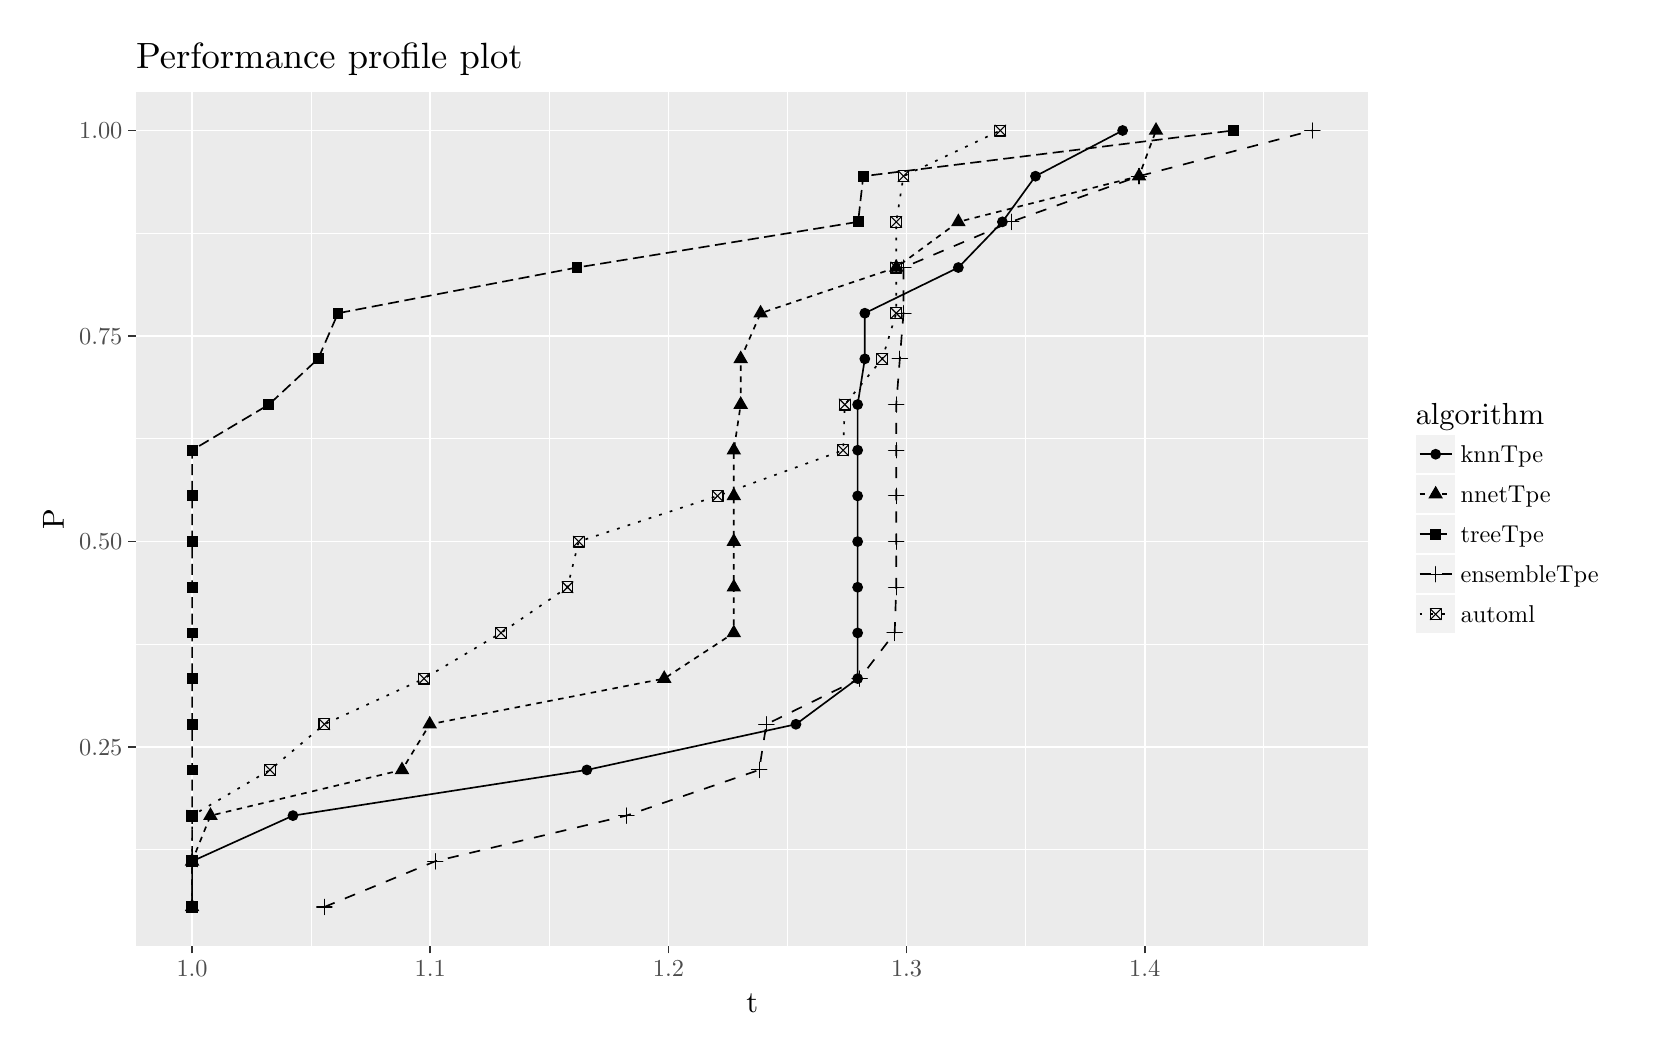
\begin{tikzpicture}[x=1pt,y=1pt]
\definecolor{fillColor}{RGB}{255,255,255}
\path[use as bounding box,fill=fillColor,fill opacity=0.00] (0,0) rectangle (578.16,361.35);
\begin{scope}
\path[clip] (  0.00,  0.00) rectangle (578.16,361.35);
\definecolor{drawColor}{RGB}{255,255,255}
\definecolor{fillColor}{RGB}{255,255,255}

\path[draw=drawColor,line width= 0.6pt,line join=round,line cap=round,fill=fillColor] (  0.00,  0.00) rectangle (578.16,361.35);
\end{scope}
\begin{scope}
\path[clip] ( 39.17, 29.59) rectangle (484.47,338.21);
\definecolor{fillColor}{gray}{0.92}

\path[fill=fillColor] ( 39.17, 29.59) rectangle (484.47,338.21);
\definecolor{drawColor}{RGB}{255,255,255}

\path[draw=drawColor,line width= 0.3pt,line join=round] ( 39.17, 64.25) --
	(484.47, 64.25);

\path[draw=drawColor,line width= 0.3pt,line join=round] ( 39.17,138.51) --
	(484.47,138.51);

\path[draw=drawColor,line width= 0.3pt,line join=round] ( 39.17,212.78) --
	(484.47,212.78);

\path[draw=drawColor,line width= 0.3pt,line join=round] ( 39.17,287.05) --
	(484.47,287.05);

\path[draw=drawColor,line width= 0.3pt,line join=round] (102.44, 29.59) --
	(102.44,338.21);

\path[draw=drawColor,line width= 0.3pt,line join=round] (188.50, 29.59) --
	(188.50,338.21);

\path[draw=drawColor,line width= 0.3pt,line join=round] (274.56, 29.59) --
	(274.56,338.21);

\path[draw=drawColor,line width= 0.3pt,line join=round] (360.62, 29.59) --
	(360.62,338.21);

\path[draw=drawColor,line width= 0.3pt,line join=round] (446.68, 29.59) --
	(446.68,338.21);

\path[draw=drawColor,line width= 0.6pt,line join=round] ( 39.17,101.38) --
	(484.47,101.38);

\path[draw=drawColor,line width= 0.6pt,line join=round] ( 39.17,175.65) --
	(484.47,175.65);

\path[draw=drawColor,line width= 0.6pt,line join=round] ( 39.17,249.92) --
	(484.47,249.92);

\path[draw=drawColor,line width= 0.6pt,line join=round] ( 39.17,324.19) --
	(484.47,324.19);

\path[draw=drawColor,line width= 0.6pt,line join=round] ( 59.41, 29.59) --
	( 59.41,338.21);

\path[draw=drawColor,line width= 0.6pt,line join=round] (145.47, 29.59) --
	(145.47,338.21);

\path[draw=drawColor,line width= 0.6pt,line join=round] (231.53, 29.59) --
	(231.53,338.21);

\path[draw=drawColor,line width= 0.6pt,line join=round] (317.59, 29.59) --
	(317.59,338.21);

\path[draw=drawColor,line width= 0.6pt,line join=round] (403.65, 29.59) --
	(403.65,338.21);
\definecolor{drawColor}{RGB}{0,0,0}

\path[draw=drawColor,line width= 0.6pt,line join=round] ( 59.41, 43.62) --
	( 59.41, 60.12) --
	( 95.86, 76.62) --
	(202.06, 93.13) --
	(277.61,109.63) --
	(299.91,126.14) --
	(299.91,142.64) --
	(299.91,159.14) --
	(299.91,175.65) --
	(299.91,192.15) --
	(299.91,208.66) --
	(299.91,225.16) --
	(302.50,241.67) --
	(302.50,258.17) --
	(336.30,274.67) --
	(352.21,291.18) --
	(364.17,307.68) --
	(395.66,324.19);

\path[draw=drawColor,line width= 0.6pt,dash pattern=on 2pt off 2pt ,line join=round] ( 59.41, 43.62) --
	( 59.41, 60.12) --
	( 66.06, 76.62) --
	(135.27, 93.13) --
	(145.28,109.63) --
	(230.01,126.14) --
	(255.16,142.64) --
	(255.16,159.14) --
	(255.16,175.65) --
	(255.16,192.15) --
	(255.16,208.66) --
	(257.65,225.16) --
	(257.65,241.67) --
	(264.84,258.17) --
	(313.85,274.67) --
	(336.30,291.18) --
	(401.58,307.68) --
	(407.72,324.19);

\path[draw=drawColor,line width= 0.6pt,dash pattern=on 4pt off 2pt ,line join=round] ( 59.41, 43.62) --
	( 59.41, 60.12) --
	( 59.41, 76.62) --
	( 59.41, 93.13) --
	( 59.41,109.63) --
	( 59.41,126.14) --
	( 59.41,142.64) --
	( 59.41,159.14) --
	( 59.41,175.65) --
	( 59.41,192.15) --
	( 59.41,208.66) --
	( 87.17,225.16) --
	(104.94,241.67) --
	(112.15,258.17) --
	(198.50,274.67) --
	(300.08,291.18) --
	(301.93,307.68) --
	(435.58,324.19);

\path[draw=drawColor,line width= 0.6pt,dash pattern=on 4pt off 4pt ,line join=round] (107.22, 43.62) --
	(147.27, 60.12) --
	(216.33, 76.62) --
	(264.31, 93.13) --
	(266.93,109.63) --
	(300.64,126.14) --
	(313.29,142.64) --
	(313.85,159.14) --
	(313.85,175.65) --
	(313.85,192.15) --
	(313.85,208.66) --
	(313.85,225.16) --
	(315.15,241.67) --
	(316.47,258.17) --
	(316.47,274.67) --
	(355.35,291.18) --
	(401.58,307.68) --
	(464.23,324.19);

\path[draw=drawColor,line width= 0.6pt,dash pattern=on 1pt off 3pt ,line join=round] ( 59.41, 43.62) --
	( 59.41, 60.12) --
	( 59.41, 76.62) --
	( 87.56, 93.13) --
	(107.22,109.63) --
	(143.22,126.14) --
	(171.03,142.64) --
	(195.06,159.14) --
	(199.09,175.65) --
	(249.29,192.15) --
	(294.68,208.66) --
	(295.26,225.16) --
	(308.80,241.67) --
	(313.85,258.17) --
	(313.85,274.67) --
	(313.85,291.18) --
	(316.47,307.68) --
	(351.46,324.19);
\definecolor{fillColor}{RGB}{0,0,0}

\path[fill=fillColor] ( 59.41, 43.62) circle (  1.96);

\path[fill=fillColor] ( 59.41, 60.12) circle (  1.96);

\path[fill=fillColor] ( 95.86, 76.62) circle (  1.96);

\path[fill=fillColor] (202.06, 93.13) circle (  1.96);

\path[fill=fillColor] (277.61,109.63) circle (  1.96);

\path[fill=fillColor] (299.91,126.14) circle (  1.96);

\path[fill=fillColor] (299.91,142.64) circle (  1.96);

\path[fill=fillColor] (299.91,159.14) circle (  1.96);

\path[fill=fillColor] (299.91,175.65) circle (  1.96);

\path[fill=fillColor] (299.91,192.15) circle (  1.96);

\path[fill=fillColor] (299.91,208.66) circle (  1.96);

\path[fill=fillColor] (299.91,225.16) circle (  1.96);

\path[fill=fillColor] (302.50,241.67) circle (  1.96);

\path[fill=fillColor] (302.50,258.17) circle (  1.96);

\path[fill=fillColor] (336.30,274.67) circle (  1.96);

\path[fill=fillColor] (352.21,291.18) circle (  1.96);

\path[fill=fillColor] (364.17,307.68) circle (  1.96);

\path[fill=fillColor] (395.66,324.19) circle (  1.96);

\path[fill=fillColor] ( 59.41, 46.67) --
	( 62.05, 42.09) --
	( 56.77, 42.09) --
	cycle;

\path[fill=fillColor] ( 59.41, 63.17) --
	( 62.05, 58.59) --
	( 56.77, 58.59) --
	cycle;

\path[fill=fillColor] ( 66.06, 79.67) --
	( 68.70, 75.10) --
	( 63.42, 75.10) --
	cycle;

\path[fill=fillColor] (135.27, 96.18) --
	(137.91, 91.60) --
	(132.62, 91.60) --
	cycle;

\path[fill=fillColor] (145.28,112.68) --
	(147.92,108.11) --
	(142.64,108.11) --
	cycle;

\path[fill=fillColor] (230.01,129.19) --
	(232.65,124.61) --
	(227.37,124.61) --
	cycle;

\path[fill=fillColor] (255.16,145.69) --
	(257.80,141.11) --
	(252.52,141.11) --
	cycle;

\path[fill=fillColor] (255.16,162.20) --
	(257.80,157.62) --
	(252.52,157.62) --
	cycle;

\path[fill=fillColor] (255.16,178.70) --
	(257.80,174.12) --
	(252.52,174.12) --
	cycle;

\path[fill=fillColor] (255.16,195.20) --
	(257.80,190.63) --
	(252.52,190.63) --
	cycle;

\path[fill=fillColor] (255.16,211.71) --
	(257.80,207.13) --
	(252.52,207.13) --
	cycle;

\path[fill=fillColor] (257.65,228.21) --
	(260.29,223.64) --
	(255.00,223.64) --
	cycle;

\path[fill=fillColor] (257.65,244.72) --
	(260.29,240.14) --
	(255.00,240.14) --
	cycle;

\path[fill=fillColor] (264.84,261.22) --
	(267.48,256.64) --
	(262.20,256.64) --
	cycle;

\path[fill=fillColor] (313.85,277.73) --
	(316.49,273.15) --
	(311.20,273.15) --
	cycle;

\path[fill=fillColor] (336.30,294.23) --
	(338.94,289.65) --
	(333.66,289.65) --
	cycle;

\path[fill=fillColor] (401.58,310.73) --
	(404.22,306.16) --
	(398.93,306.16) --
	cycle;

\path[fill=fillColor] (407.72,327.24) --
	(410.36,322.66) --
	(405.07,322.66) --
	cycle;

\path[fill=fillColor] ( 57.45, 41.65) --
	( 61.37, 41.65) --
	( 61.37, 45.58) --
	( 57.45, 45.58) --
	cycle;

\path[fill=fillColor] ( 57.45, 58.16) --
	( 61.37, 58.16) --
	( 61.37, 62.08) --
	( 57.45, 62.08) --
	cycle;

\path[fill=fillColor] ( 57.45, 74.66) --
	( 61.37, 74.66) --
	( 61.37, 78.59) --
	( 57.45, 78.59) --
	cycle;

\path[fill=fillColor] ( 57.45, 91.17) --
	( 61.37, 91.17) --
	( 61.37, 95.09) --
	( 57.45, 95.09) --
	cycle;

\path[fill=fillColor] ( 57.45,107.67) --
	( 61.37,107.67) --
	( 61.37,111.59) --
	( 57.45,111.59) --
	cycle;

\path[fill=fillColor] ( 57.45,124.17) --
	( 61.37,124.17) --
	( 61.37,128.10) --
	( 57.45,128.10) --
	cycle;

\path[fill=fillColor] ( 57.45,140.68) --
	( 61.37,140.68) --
	( 61.37,144.60) --
	( 57.45,144.60) --
	cycle;

\path[fill=fillColor] ( 57.45,157.18) --
	( 61.37,157.18) --
	( 61.37,161.11) --
	( 57.45,161.11) --
	cycle;

\path[fill=fillColor] ( 57.45,173.69) --
	( 61.37,173.69) --
	( 61.37,177.61) --
	( 57.45,177.61) --
	cycle;

\path[fill=fillColor] ( 57.45,190.19) --
	( 61.37,190.19) --
	( 61.37,194.12) --
	( 57.45,194.12) --
	cycle;

\path[fill=fillColor] ( 57.45,206.69) --
	( 61.37,206.69) --
	( 61.37,210.62) --
	( 57.45,210.62) --
	cycle;

\path[fill=fillColor] ( 85.21,223.20) --
	( 89.13,223.20) --
	( 89.13,227.12) --
	( 85.21,227.12) --
	cycle;

\path[fill=fillColor] (102.98,239.70) --
	(106.90,239.70) --
	(106.90,243.63) --
	(102.98,243.63) --
	cycle;

\path[fill=fillColor] (110.18,256.21) --
	(114.11,256.21) --
	(114.11,260.13) --
	(110.18,260.13) --
	cycle;

\path[fill=fillColor] (196.54,272.71) --
	(200.47,272.71) --
	(200.47,276.64) --
	(196.54,276.64) --
	cycle;

\path[fill=fillColor] (298.12,289.22) --
	(302.05,289.22) --
	(302.05,293.14) --
	(298.12,293.14) --
	cycle;

\path[fill=fillColor] (299.97,305.72) --
	(303.89,305.72) --
	(303.89,309.64) --
	(299.97,309.64) --
	cycle;

\path[fill=fillColor] (433.62,322.22) --
	(437.54,322.22) --
	(437.54,326.15) --
	(433.62,326.15) --
	cycle;

\path[draw=drawColor,line width= 0.4pt,line join=round,line cap=round] (104.44, 43.62) -- (109.99, 43.62);

\path[draw=drawColor,line width= 0.4pt,line join=round,line cap=round] (107.22, 40.84) -- (107.22, 46.39);

\path[draw=drawColor,line width= 0.4pt,line join=round,line cap=round] (144.50, 60.12) -- (150.05, 60.12);

\path[draw=drawColor,line width= 0.4pt,line join=round,line cap=round] (147.27, 57.34) -- (147.27, 62.89);

\path[draw=drawColor,line width= 0.4pt,line join=round,line cap=round] (213.56, 76.62) -- (219.11, 76.62);

\path[draw=drawColor,line width= 0.4pt,line join=round,line cap=round] (216.33, 73.85) -- (216.33, 79.40);

\path[draw=drawColor,line width= 0.4pt,line join=round,line cap=round] (261.53, 93.13) -- (267.08, 93.13);

\path[draw=drawColor,line width= 0.4pt,line join=round,line cap=round] (264.31, 90.35) -- (264.31, 95.90);

\path[draw=drawColor,line width= 0.4pt,line join=round,line cap=round] (264.16,109.63) -- (269.71,109.63);

\path[draw=drawColor,line width= 0.4pt,line join=round,line cap=round] (266.93,106.86) -- (266.93,112.41);

\path[draw=drawColor,line width= 0.4pt,line join=round,line cap=round] (297.86,126.14) -- (303.41,126.14);

\path[draw=drawColor,line width= 0.4pt,line join=round,line cap=round] (300.64,123.36) -- (300.64,128.91);

\path[draw=drawColor,line width= 0.4pt,line join=round,line cap=round] (310.52,142.64) -- (316.07,142.64);

\path[draw=drawColor,line width= 0.4pt,line join=round,line cap=round] (313.29,139.87) -- (313.29,145.42);

\path[draw=drawColor,line width= 0.4pt,line join=round,line cap=round] (311.07,159.14) -- (316.62,159.14);

\path[draw=drawColor,line width= 0.4pt,line join=round,line cap=round] (313.85,156.37) -- (313.85,161.92);

\path[draw=drawColor,line width= 0.4pt,line join=round,line cap=round] (311.07,175.65) -- (316.62,175.65);

\path[draw=drawColor,line width= 0.4pt,line join=round,line cap=round] (313.85,172.87) -- (313.85,178.42);

\path[draw=drawColor,line width= 0.4pt,line join=round,line cap=round] (311.07,192.15) -- (316.62,192.15);

\path[draw=drawColor,line width= 0.4pt,line join=round,line cap=round] (313.85,189.38) -- (313.85,194.93);

\path[draw=drawColor,line width= 0.4pt,line join=round,line cap=round] (311.07,208.66) -- (316.62,208.66);

\path[draw=drawColor,line width= 0.4pt,line join=round,line cap=round] (313.85,205.88) -- (313.85,211.43);

\path[draw=drawColor,line width= 0.4pt,line join=round,line cap=round] (311.07,225.16) -- (316.62,225.16);

\path[draw=drawColor,line width= 0.4pt,line join=round,line cap=round] (313.85,222.39) -- (313.85,227.94);

\path[draw=drawColor,line width= 0.4pt,line join=round,line cap=round] (312.38,241.67) -- (317.93,241.67);

\path[draw=drawColor,line width= 0.4pt,line join=round,line cap=round] (315.15,238.89) -- (315.15,244.44);

\path[draw=drawColor,line width= 0.4pt,line join=round,line cap=round] (313.70,258.17) -- (319.25,258.17);

\path[draw=drawColor,line width= 0.4pt,line join=round,line cap=round] (316.47,255.39) -- (316.47,260.94);

\path[draw=drawColor,line width= 0.4pt,line join=round,line cap=round] (313.70,274.67) -- (319.25,274.67);

\path[draw=drawColor,line width= 0.4pt,line join=round,line cap=round] (316.47,271.90) -- (316.47,277.45);

\path[draw=drawColor,line width= 0.4pt,line join=round,line cap=round] (352.57,291.18) -- (358.12,291.18);

\path[draw=drawColor,line width= 0.4pt,line join=round,line cap=round] (355.35,288.40) -- (355.35,293.95);

\path[draw=drawColor,line width= 0.4pt,line join=round,line cap=round] (398.80,307.68) -- (404.35,307.68);

\path[draw=drawColor,line width= 0.4pt,line join=round,line cap=round] (401.58,304.91) -- (401.58,310.46);

\path[draw=drawColor,line width= 0.4pt,line join=round,line cap=round] (461.45,324.19) -- (467.00,324.19);

\path[draw=drawColor,line width= 0.4pt,line join=round,line cap=round] (464.23,321.41) -- (464.23,326.96);

\path[draw=drawColor,line width= 0.4pt,line join=round,line cap=round] ( 57.45, 41.65) rectangle ( 61.37, 45.58);

\path[draw=drawColor,line width= 0.4pt,line join=round,line cap=round] ( 57.45, 41.65) -- ( 61.37, 45.58);

\path[draw=drawColor,line width= 0.4pt,line join=round,line cap=round] ( 57.45, 45.58) -- ( 61.37, 41.65);

\path[draw=drawColor,line width= 0.4pt,line join=round,line cap=round] ( 57.45, 58.16) rectangle ( 61.37, 62.08);

\path[draw=drawColor,line width= 0.4pt,line join=round,line cap=round] ( 57.45, 58.16) -- ( 61.37, 62.08);

\path[draw=drawColor,line width= 0.4pt,line join=round,line cap=round] ( 57.45, 62.08) -- ( 61.37, 58.16);

\path[draw=drawColor,line width= 0.4pt,line join=round,line cap=round] ( 57.45, 74.66) rectangle ( 61.37, 78.59);

\path[draw=drawColor,line width= 0.4pt,line join=round,line cap=round] ( 57.45, 74.66) -- ( 61.37, 78.59);

\path[draw=drawColor,line width= 0.4pt,line join=round,line cap=round] ( 57.45, 78.59) -- ( 61.37, 74.66);

\path[draw=drawColor,line width= 0.4pt,line join=round,line cap=round] ( 85.60, 91.17) rectangle ( 89.52, 95.09);

\path[draw=drawColor,line width= 0.4pt,line join=round,line cap=round] ( 85.60, 91.17) -- ( 89.52, 95.09);

\path[draw=drawColor,line width= 0.4pt,line join=round,line cap=round] ( 85.60, 95.09) -- ( 89.52, 91.17);

\path[draw=drawColor,line width= 0.4pt,line join=round,line cap=round] (105.26,107.67) rectangle (109.18,111.59);

\path[draw=drawColor,line width= 0.4pt,line join=round,line cap=round] (105.26,107.67) -- (109.18,111.59);

\path[draw=drawColor,line width= 0.4pt,line join=round,line cap=round] (105.26,111.59) -- (109.18,107.67);

\path[draw=drawColor,line width= 0.4pt,line join=round,line cap=round] (141.25,124.17) rectangle (145.18,128.10);

\path[draw=drawColor,line width= 0.4pt,line join=round,line cap=round] (141.25,124.17) -- (145.18,128.10);

\path[draw=drawColor,line width= 0.4pt,line join=round,line cap=round] (141.25,128.10) -- (145.18,124.17);

\path[draw=drawColor,line width= 0.4pt,line join=round,line cap=round] (169.07,140.68) rectangle (172.99,144.60);

\path[draw=drawColor,line width= 0.4pt,line join=round,line cap=round] (169.07,140.68) -- (172.99,144.60);

\path[draw=drawColor,line width= 0.4pt,line join=round,line cap=round] (169.07,144.60) -- (172.99,140.68);

\path[draw=drawColor,line width= 0.4pt,line join=round,line cap=round] (193.10,157.18) rectangle (197.02,161.11);

\path[draw=drawColor,line width= 0.4pt,line join=round,line cap=round] (193.10,157.18) -- (197.02,161.11);

\path[draw=drawColor,line width= 0.4pt,line join=round,line cap=round] (193.10,161.11) -- (197.02,157.18);

\path[draw=drawColor,line width= 0.4pt,line join=round,line cap=round] (197.13,173.69) rectangle (201.05,177.61);

\path[draw=drawColor,line width= 0.4pt,line join=round,line cap=round] (197.13,173.69) -- (201.05,177.61);

\path[draw=drawColor,line width= 0.4pt,line join=round,line cap=round] (197.13,177.61) -- (201.05,173.69);

\path[draw=drawColor,line width= 0.4pt,line join=round,line cap=round] (247.33,190.19) rectangle (251.25,194.12);

\path[draw=drawColor,line width= 0.4pt,line join=round,line cap=round] (247.33,190.19) -- (251.25,194.12);

\path[draw=drawColor,line width= 0.4pt,line join=round,line cap=round] (247.33,194.12) -- (251.25,190.19);

\path[draw=drawColor,line width= 0.4pt,line join=round,line cap=round] (292.71,206.69) rectangle (296.64,210.62);

\path[draw=drawColor,line width= 0.4pt,line join=round,line cap=round] (292.71,206.69) -- (296.64,210.62);

\path[draw=drawColor,line width= 0.4pt,line join=round,line cap=round] (292.71,210.62) -- (296.64,206.69);

\path[draw=drawColor,line width= 0.4pt,line join=round,line cap=round] (293.30,223.20) rectangle (297.23,227.12);

\path[draw=drawColor,line width= 0.4pt,line join=round,line cap=round] (293.30,223.20) -- (297.23,227.12);

\path[draw=drawColor,line width= 0.4pt,line join=round,line cap=round] (293.30,227.12) -- (297.23,223.20);

\path[draw=drawColor,line width= 0.4pt,line join=round,line cap=round] (306.84,239.70) rectangle (310.77,243.63);

\path[draw=drawColor,line width= 0.4pt,line join=round,line cap=round] (306.84,239.70) -- (310.77,243.63);

\path[draw=drawColor,line width= 0.4pt,line join=round,line cap=round] (306.84,243.63) -- (310.77,239.70);

\path[draw=drawColor,line width= 0.4pt,line join=round,line cap=round] (311.89,256.21) rectangle (315.81,260.13);

\path[draw=drawColor,line width= 0.4pt,line join=round,line cap=round] (311.89,256.21) -- (315.81,260.13);

\path[draw=drawColor,line width= 0.4pt,line join=round,line cap=round] (311.89,260.13) -- (315.81,256.21);

\path[draw=drawColor,line width= 0.4pt,line join=round,line cap=round] (311.89,272.71) rectangle (315.81,276.64);

\path[draw=drawColor,line width= 0.4pt,line join=round,line cap=round] (311.89,272.71) -- (315.81,276.64);

\path[draw=drawColor,line width= 0.4pt,line join=round,line cap=round] (311.89,276.64) -- (315.81,272.71);

\path[draw=drawColor,line width= 0.4pt,line join=round,line cap=round] (311.89,289.22) rectangle (315.81,293.14);

\path[draw=drawColor,line width= 0.4pt,line join=round,line cap=round] (311.89,289.22) -- (315.81,293.14);

\path[draw=drawColor,line width= 0.4pt,line join=round,line cap=round] (311.89,293.14) -- (315.81,289.22);

\path[draw=drawColor,line width= 0.4pt,line join=round,line cap=round] (314.51,305.72) rectangle (318.43,309.64);

\path[draw=drawColor,line width= 0.4pt,line join=round,line cap=round] (314.51,305.72) -- (318.43,309.64);

\path[draw=drawColor,line width= 0.4pt,line join=round,line cap=round] (314.51,309.64) -- (318.43,305.72);

\path[draw=drawColor,line width= 0.4pt,line join=round,line cap=round] (349.50,322.22) rectangle (353.42,326.15);

\path[draw=drawColor,line width= 0.4pt,line join=round,line cap=round] (349.50,322.22) -- (353.42,326.15);

\path[draw=drawColor,line width= 0.4pt,line join=round,line cap=round] (349.50,326.15) -- (353.42,322.22);
\end{scope}
\begin{scope}
\path[clip] (  0.00,  0.00) rectangle (578.16,361.35);
\definecolor{drawColor}{gray}{0.30}

\node[text=drawColor,anchor=base east,inner sep=0pt, outer sep=0pt, scale=  0.88] at ( 34.22, 98.35) {0.25};

\node[text=drawColor,anchor=base east,inner sep=0pt, outer sep=0pt, scale=  0.88] at ( 34.22,172.62) {0.50};

\node[text=drawColor,anchor=base east,inner sep=0pt, outer sep=0pt, scale=  0.88] at ( 34.22,246.89) {0.75};

\node[text=drawColor,anchor=base east,inner sep=0pt, outer sep=0pt, scale=  0.88] at ( 34.22,321.16) {1.00};
\end{scope}
\begin{scope}
\path[clip] (  0.00,  0.00) rectangle (578.16,361.35);
\definecolor{drawColor}{gray}{0.20}

\path[draw=drawColor,line width= 0.6pt,line join=round] ( 36.42,101.38) --
	( 39.17,101.38);

\path[draw=drawColor,line width= 0.6pt,line join=round] ( 36.42,175.65) --
	( 39.17,175.65);

\path[draw=drawColor,line width= 0.6pt,line join=round] ( 36.42,249.92) --
	( 39.17,249.92);

\path[draw=drawColor,line width= 0.6pt,line join=round] ( 36.42,324.19) --
	( 39.17,324.19);
\end{scope}
\begin{scope}
\path[clip] (  0.00,  0.00) rectangle (578.16,361.35);
\definecolor{drawColor}{gray}{0.20}

\path[draw=drawColor,line width= 0.6pt,line join=round] ( 59.41, 26.84) --
	( 59.41, 29.59);

\path[draw=drawColor,line width= 0.6pt,line join=round] (145.47, 26.84) --
	(145.47, 29.59);

\path[draw=drawColor,line width= 0.6pt,line join=round] (231.53, 26.84) --
	(231.53, 29.59);

\path[draw=drawColor,line width= 0.6pt,line join=round] (317.59, 26.84) --
	(317.59, 29.59);

\path[draw=drawColor,line width= 0.6pt,line join=round] (403.65, 26.84) --
	(403.65, 29.59);
\end{scope}
\begin{scope}
\path[clip] (  0.00,  0.00) rectangle (578.16,361.35);
\definecolor{drawColor}{gray}{0.30}

\node[text=drawColor,anchor=base,inner sep=0pt, outer sep=0pt, scale=  0.88] at ( 59.41, 18.58) {1.0};

\node[text=drawColor,anchor=base,inner sep=0pt, outer sep=0pt, scale=  0.88] at (145.47, 18.58) {1.1};

\node[text=drawColor,anchor=base,inner sep=0pt, outer sep=0pt, scale=  0.88] at (231.53, 18.58) {1.2};

\node[text=drawColor,anchor=base,inner sep=0pt, outer sep=0pt, scale=  0.88] at (317.59, 18.58) {1.3};

\node[text=drawColor,anchor=base,inner sep=0pt, outer sep=0pt, scale=  0.88] at (403.65, 18.58) {1.4};
\end{scope}
\begin{scope}
\path[clip] (  0.00,  0.00) rectangle (578.16,361.35);
\definecolor{drawColor}{RGB}{0,0,0}

\node[text=drawColor,anchor=base,inner sep=0pt, outer sep=0pt, scale=  1.10] at (261.82,  5.50) {t};
\end{scope}
\begin{scope}
\path[clip] (  0.00,  0.00) rectangle (578.16,361.35);
\definecolor{drawColor}{RGB}{0,0,0}

\node[text=drawColor,rotate= 90.00,anchor=base,inner sep=0pt, outer sep=0pt, scale=  1.10] at ( 13.08,183.90) {P};
\end{scope}
\begin{scope}
\path[clip] (  0.00,  0.00) rectangle (578.16,361.35);
\definecolor{fillColor}{RGB}{255,255,255}

\path[fill=fillColor] (495.85,136.48) rectangle (572.66,231.32);
\end{scope}
\begin{scope}
\path[clip] (  0.00,  0.00) rectangle (578.16,361.35);
\definecolor{drawColor}{RGB}{0,0,0}

\node[text=drawColor,anchor=base west,inner sep=0pt, outer sep=0pt, scale=  1.10] at (501.54,218.05) {algorithm};
\end{scope}
\begin{scope}
\path[clip] (  0.00,  0.00) rectangle (578.16,361.35);
\definecolor{drawColor}{RGB}{255,255,255}
\definecolor{fillColor}{gray}{0.95}

\path[draw=drawColor,line width= 0.6pt,line join=round,line cap=round,fill=fillColor] (501.54,199.99) rectangle (515.99,214.44);
\end{scope}
\begin{scope}
\path[clip] (  0.00,  0.00) rectangle (578.16,361.35);
\definecolor{drawColor}{RGB}{0,0,0}

\path[draw=drawColor,line width= 0.6pt,line join=round] (502.98,207.21) -- (514.55,207.21);
\end{scope}
\begin{scope}
\path[clip] (  0.00,  0.00) rectangle (578.16,361.35);
\definecolor{fillColor}{RGB}{0,0,0}

\path[fill=fillColor] (508.77,207.21) circle (  1.96);
\end{scope}
\begin{scope}
\path[clip] (  0.00,  0.00) rectangle (578.16,361.35);
\definecolor{drawColor}{RGB}{255,255,255}
\definecolor{fillColor}{gray}{0.95}

\path[draw=drawColor,line width= 0.6pt,line join=round,line cap=round,fill=fillColor] (501.54,185.53) rectangle (515.99,199.99);
\end{scope}
\begin{scope}
\path[clip] (  0.00,  0.00) rectangle (578.16,361.35);
\definecolor{drawColor}{RGB}{0,0,0}

\path[draw=drawColor,line width= 0.6pt,dash pattern=on 2pt off 2pt ,line join=round] (502.98,192.76) -- (514.55,192.76);
\end{scope}
\begin{scope}
\path[clip] (  0.00,  0.00) rectangle (578.16,361.35);
\definecolor{fillColor}{RGB}{0,0,0}

\path[fill=fillColor] (508.77,195.81) --
	(511.41,191.23) --
	(506.12,191.23) --
	cycle;
\end{scope}
\begin{scope}
\path[clip] (  0.00,  0.00) rectangle (578.16,361.35);
\definecolor{drawColor}{RGB}{255,255,255}
\definecolor{fillColor}{gray}{0.95}

\path[draw=drawColor,line width= 0.6pt,line join=round,line cap=round,fill=fillColor] (501.54,171.08) rectangle (515.99,185.53);
\end{scope}
\begin{scope}
\path[clip] (  0.00,  0.00) rectangle (578.16,361.35);
\definecolor{drawColor}{RGB}{0,0,0}

\path[draw=drawColor,line width= 0.6pt,dash pattern=on 4pt off 2pt ,line join=round] (502.98,178.31) -- (514.55,178.31);
\end{scope}
\begin{scope}
\path[clip] (  0.00,  0.00) rectangle (578.16,361.35);
\definecolor{fillColor}{RGB}{0,0,0}

\path[fill=fillColor] (506.80,176.34) --
	(510.73,176.34) --
	(510.73,180.27) --
	(506.80,180.27) --
	cycle;
\end{scope}
\begin{scope}
\path[clip] (  0.00,  0.00) rectangle (578.16,361.35);
\definecolor{drawColor}{RGB}{255,255,255}
\definecolor{fillColor}{gray}{0.95}

\path[draw=drawColor,line width= 0.6pt,line join=round,line cap=round,fill=fillColor] (501.54,156.63) rectangle (515.99,171.08);
\end{scope}
\begin{scope}
\path[clip] (  0.00,  0.00) rectangle (578.16,361.35);
\definecolor{drawColor}{RGB}{0,0,0}

\path[draw=drawColor,line width= 0.6pt,dash pattern=on 4pt off 4pt ,line join=round] (502.98,163.85) -- (514.55,163.85);
\end{scope}
\begin{scope}
\path[clip] (  0.00,  0.00) rectangle (578.16,361.35);
\definecolor{drawColor}{RGB}{0,0,0}

\path[draw=drawColor,line width= 0.4pt,line join=round,line cap=round] (505.99,163.85) -- (511.54,163.85);

\path[draw=drawColor,line width= 0.4pt,line join=round,line cap=round] (508.77,161.08) -- (508.77,166.63);
\end{scope}
\begin{scope}
\path[clip] (  0.00,  0.00) rectangle (578.16,361.35);
\definecolor{drawColor}{RGB}{255,255,255}
\definecolor{fillColor}{gray}{0.95}

\path[draw=drawColor,line width= 0.6pt,line join=round,line cap=round,fill=fillColor] (501.54,142.17) rectangle (515.99,156.63);
\end{scope}
\begin{scope}
\path[clip] (  0.00,  0.00) rectangle (578.16,361.35);
\definecolor{drawColor}{RGB}{0,0,0}

\path[draw=drawColor,line width= 0.6pt,dash pattern=on 1pt off 3pt ,line join=round] (502.98,149.40) -- (514.55,149.40);
\end{scope}
\begin{scope}
\path[clip] (  0.00,  0.00) rectangle (578.16,361.35);
\definecolor{drawColor}{RGB}{0,0,0}

\path[draw=drawColor,line width= 0.4pt,line join=round,line cap=round] (506.80,147.44) rectangle (510.73,151.36);

\path[draw=drawColor,line width= 0.4pt,line join=round,line cap=round] (506.80,147.44) -- (510.73,151.36);

\path[draw=drawColor,line width= 0.4pt,line join=round,line cap=round] (506.80,151.36) -- (510.73,147.44);
\end{scope}
\begin{scope}
\path[clip] (  0.00,  0.00) rectangle (578.16,361.35);
\definecolor{drawColor}{RGB}{0,0,0}

\node[text=drawColor,anchor=base west,inner sep=0pt, outer sep=0pt, scale=  0.88] at (517.80,204.18) {knnTpe};
\end{scope}
\begin{scope}
\path[clip] (  0.00,  0.00) rectangle (578.16,361.35);
\definecolor{drawColor}{RGB}{0,0,0}

\node[text=drawColor,anchor=base west,inner sep=0pt, outer sep=0pt, scale=  0.88] at (517.80,189.73) {nnetTpe};
\end{scope}
\begin{scope}
\path[clip] (  0.00,  0.00) rectangle (578.16,361.35);
\definecolor{drawColor}{RGB}{0,0,0}

\node[text=drawColor,anchor=base west,inner sep=0pt, outer sep=0pt, scale=  0.88] at (517.80,175.28) {treeTpe};
\end{scope}
\begin{scope}
\path[clip] (  0.00,  0.00) rectangle (578.16,361.35);
\definecolor{drawColor}{RGB}{0,0,0}

\node[text=drawColor,anchor=base west,inner sep=0pt, outer sep=0pt, scale=  0.88] at (517.80,160.82) {ensembleTpe};
\end{scope}
\begin{scope}
\path[clip] (  0.00,  0.00) rectangle (578.16,361.35);
\definecolor{drawColor}{RGB}{0,0,0}

\node[text=drawColor,anchor=base west,inner sep=0pt, outer sep=0pt, scale=  0.88] at (517.80,146.37) {automl};
\end{scope}
\begin{scope}
\path[clip] (  0.00,  0.00) rectangle (578.16,361.35);
\definecolor{drawColor}{RGB}{0,0,0}

\node[text=drawColor,anchor=base west,inner sep=0pt, outer sep=0pt, scale=  1.32] at ( 39.17,346.76) {Performance profile plot};
\end{scope}
\end{tikzpicture}

}
	\caption{Διάγραμμα προφίλ απόδοσης συνολικού συστήματος}
	\label{fig:systemproftpe}
\end{figure}
	
\paragraph{Συμπεράσματα}
Με τη βοήθεια του Πίνακα \ref{table:pvalues} μπορούμε να αναγνωρίσουμε τα ζεύγη αλγορίθμων που παρουσιάζουν σημαντική διαφορετική απόδοση στα σετ δεδομένων ελέγχου. Το σύστημά μας διαφέρει σημαντικά μόνο με τις μεθόδους ensembleGrid και ensembleTpe.
Επίσης, σύμφωνα με τα Σχήματα \ref{fig:systemprofgrid} και \ref{fig:systemproftpe} η μέθοδος με την καλύτερη απόδοση σε όλα τα σετ δεδομένων είναι η , ενώ το σύστημά μας . 

Το σύστημά μας είναι εξίσου αποδοτικό με τις τρέχουσες τεχνικές σχεδόν σε όλα τα σετ εκπαίδευσης ελέγχου. Επίσης, έχει επιτευχθεί η αντικατάσταση της χρονοβόρας βελτιστοποίησης υπερ-παραμέτρων με απλή πρόβλεψη και η δημιουργία μετα-γνώσης, χαρακτηριστικά που δε συνδέονται άμεσα με την απόδοση του συστήματος, ωστόσο επιφέρουν υπολογιστικά οφέλη και δυνατότητες εκμετάλλευσης. Συμπεραίνουμε επομένως πως το σύστημά μας αποτελεί χρήσιμη προσθήκη στο σύνολο των \gls{AutoML} εργαλείων. 